%------------------------------------------------------------------------------
\chapter{Useful information}
\label{sec:app}
%------------------------------------------------------------------------------

\section*{}

\begin{table}[h!]
     \centering
      \begin{tabular}{@{} *4l  @{}}
      \toprule
      Region & Distribution & Additional Info  \\
     \midrule
      SR 2j1b & $O_{NN}$ < 0.4 & {--}\\[0.2ex]
      SR 3j1b & $O_{NN}$ < 0.4 & {--}\\[0.2ex]
      CR diboson 2j0b & $m_{T}(\ell,E_{T}^{miss})$ & No change \\[0.2ex]
      CR diboson 3j0b & $m_{T}(\ell,E_{T}^{miss})$ & No change \\[0.2ex]
      CR $t\Bar{t}$ 2j1b & $m_{bj_{f}}$ & No change \\[0.2ex]
      CR $t\Bar{t}$ 3j1b & $m_{bj_{f}}$ & No change \\[0.2ex]
      CR $t\Bar{t}Z$ 3j2b & $O_{NN}$ < 0.6 & {--}\\[0.2ex]
      CR $t\Bar{t}Z$ 4j2b & $O_{NN}$ < 0.6 & {--}\\[0.2ex]
      \bottomrule
 \end{tabular}
 \caption{Overview of the regions included in the background only fit}
 \label{tab:backgroundonlyfit}
 \end{table}
 
 
\begin{figure}[!h]
  \begin{subfigure}[b]{0.33\linewidth}
    \centering
    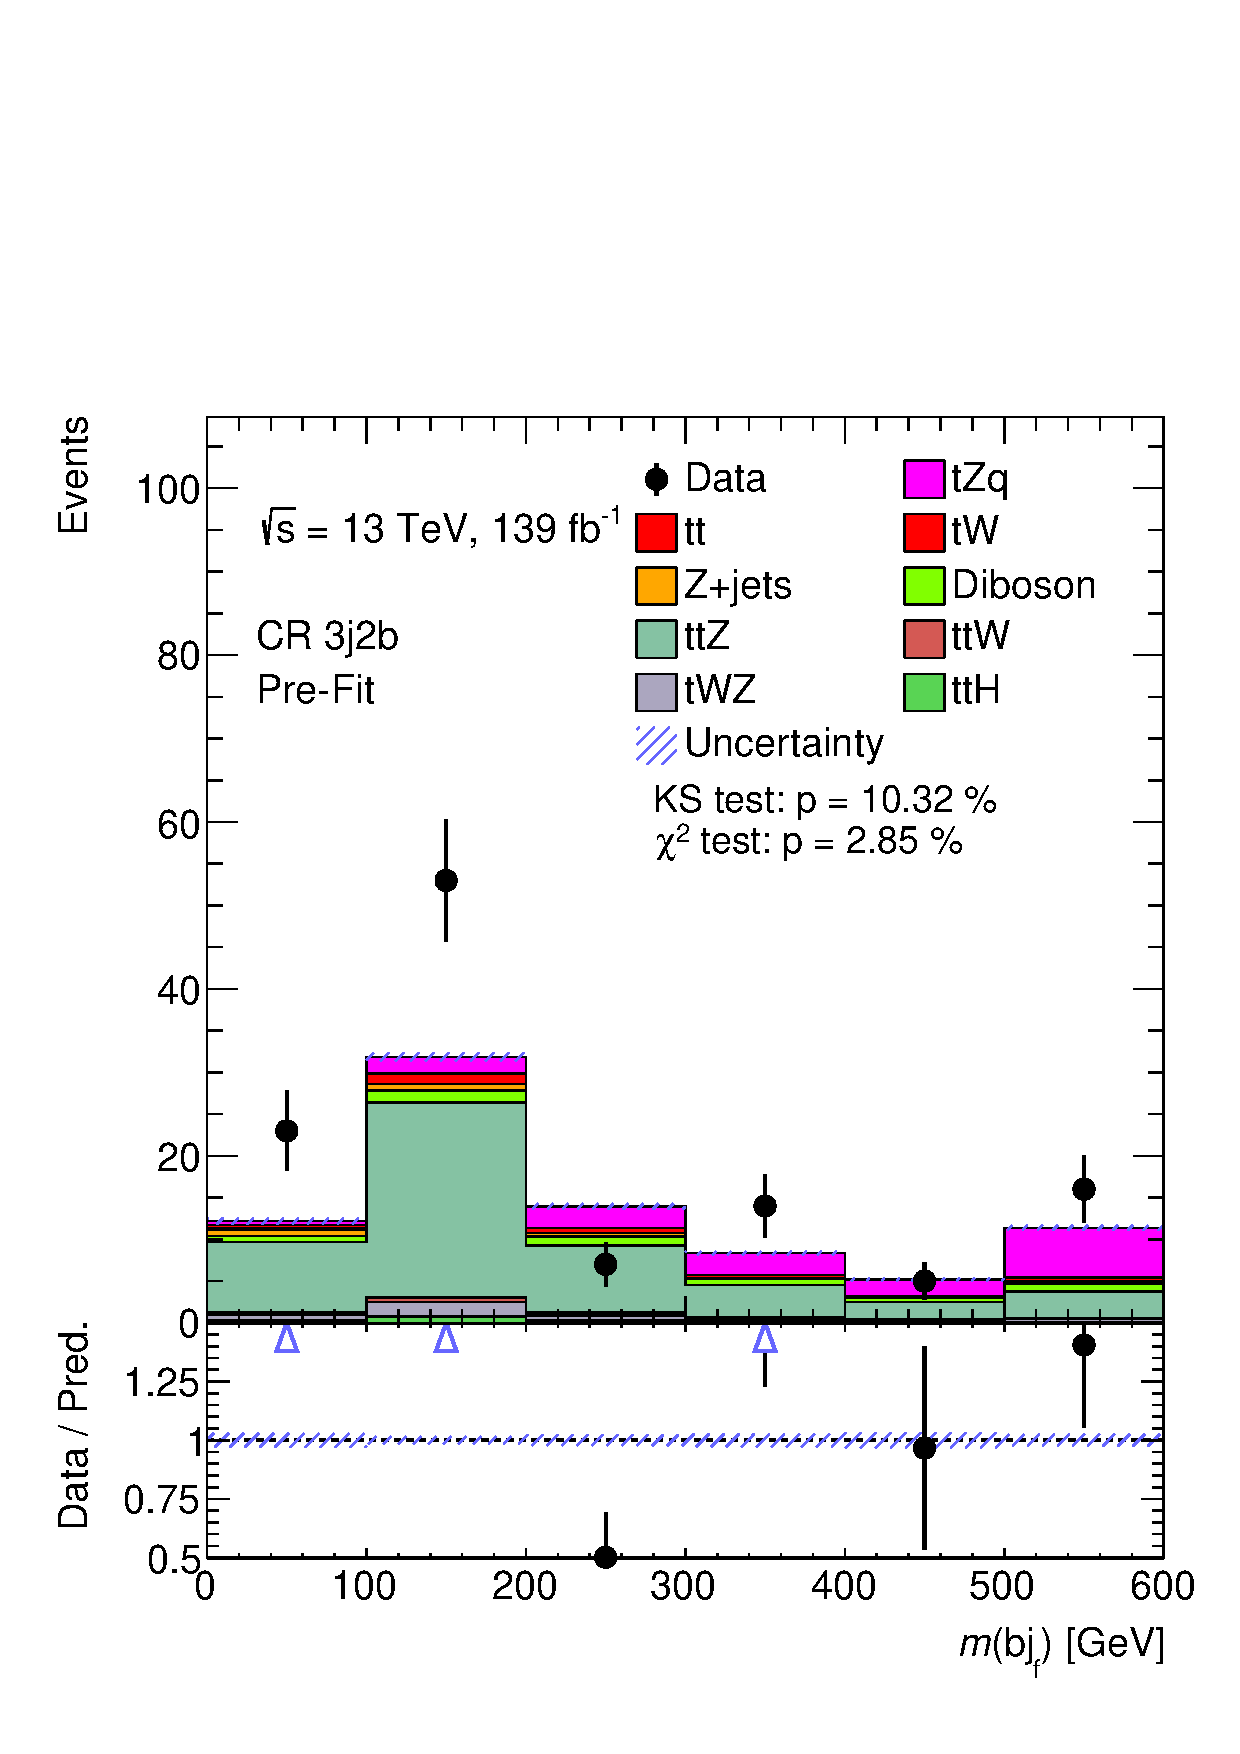
\includegraphics[width=\linewidth]{ubonn-thesis/Chapters/Chapters_06/Figure/Input_distribution/CR_3j2b_M_bj.pdf} 
  \end{subfigure}%% 
  \begin{subfigure}[b]{0.33\linewidth}
    \centering
    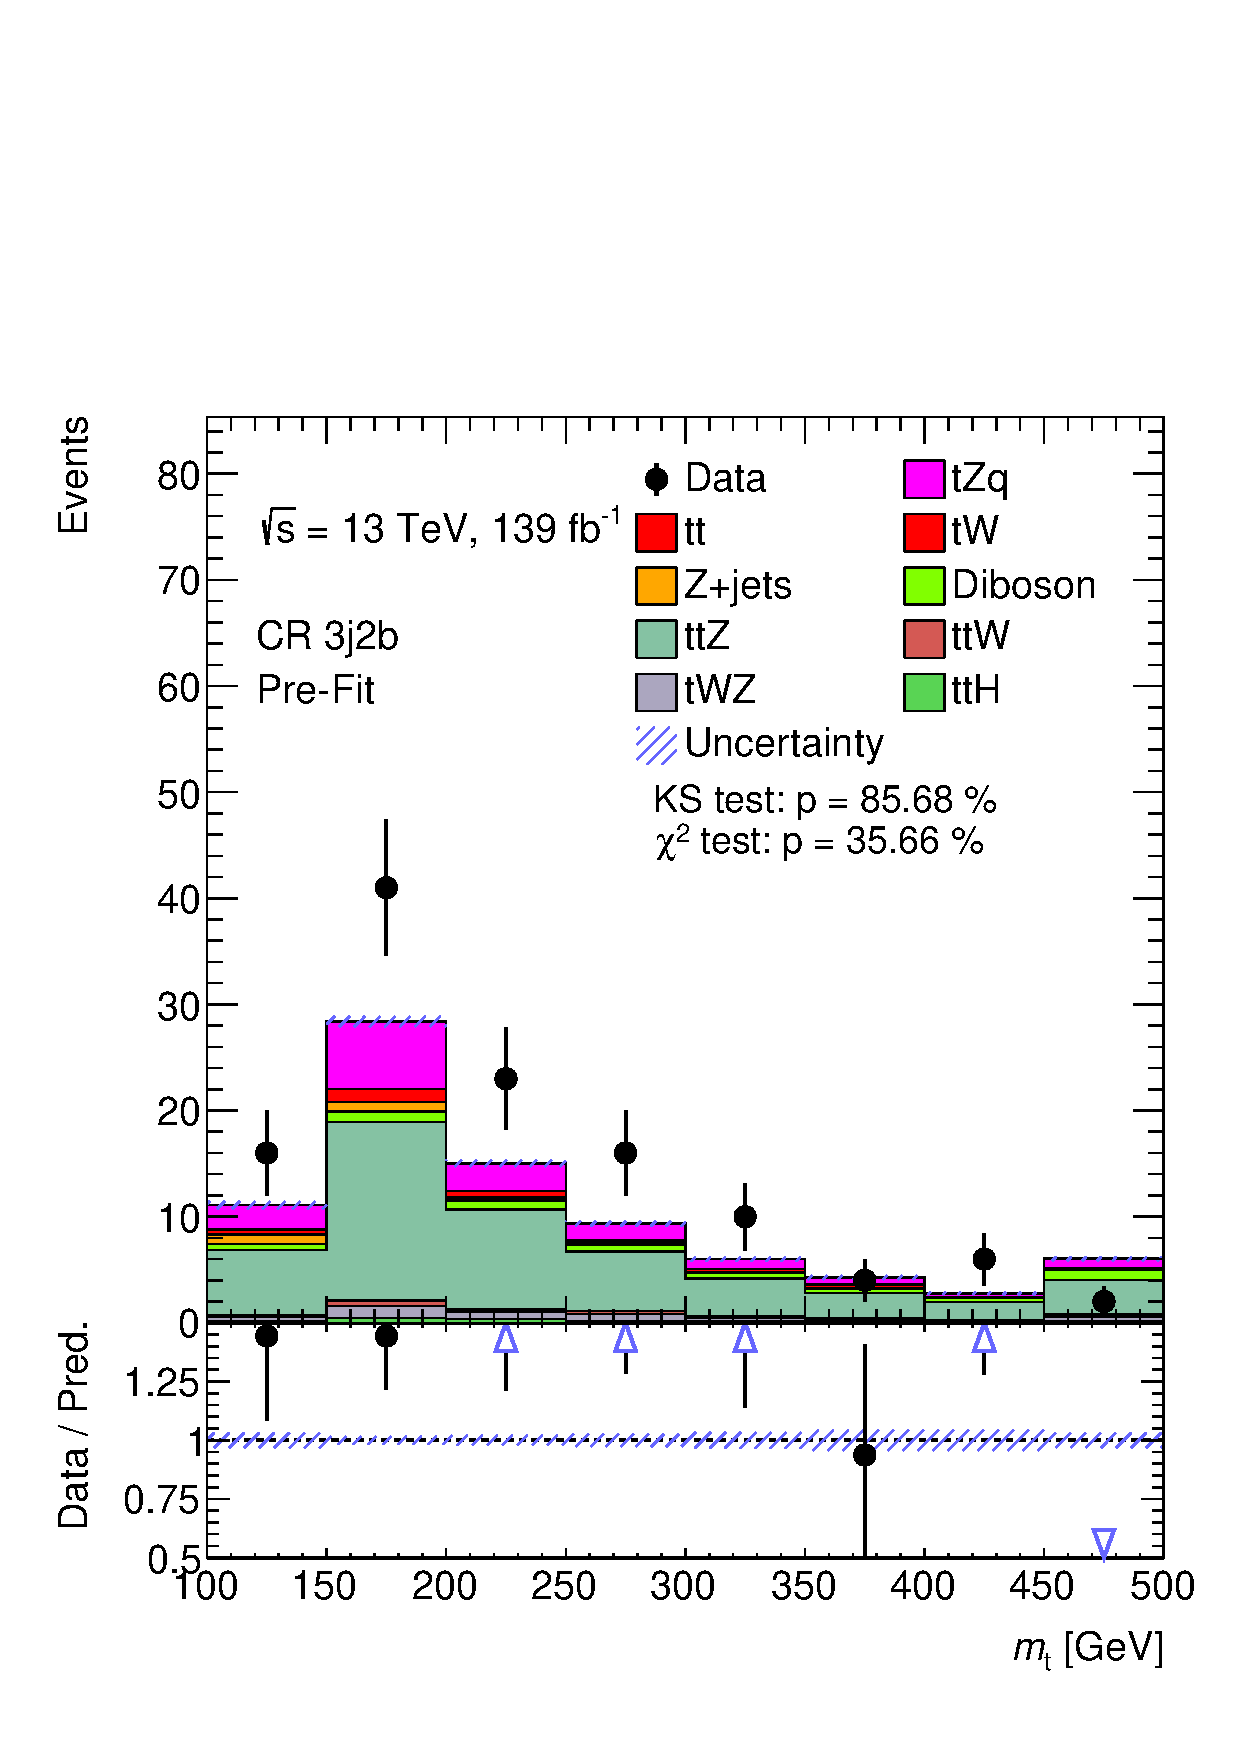
\includegraphics[width=\linewidth]{ubonn-thesis/Chapters/Chapters_06/Figure/Input_distribution/CR_3j2b_Top_mass.pdf} 
  \end{subfigure} 
  \begin{subfigure}[b]{0.33\linewidth}
    \centering
    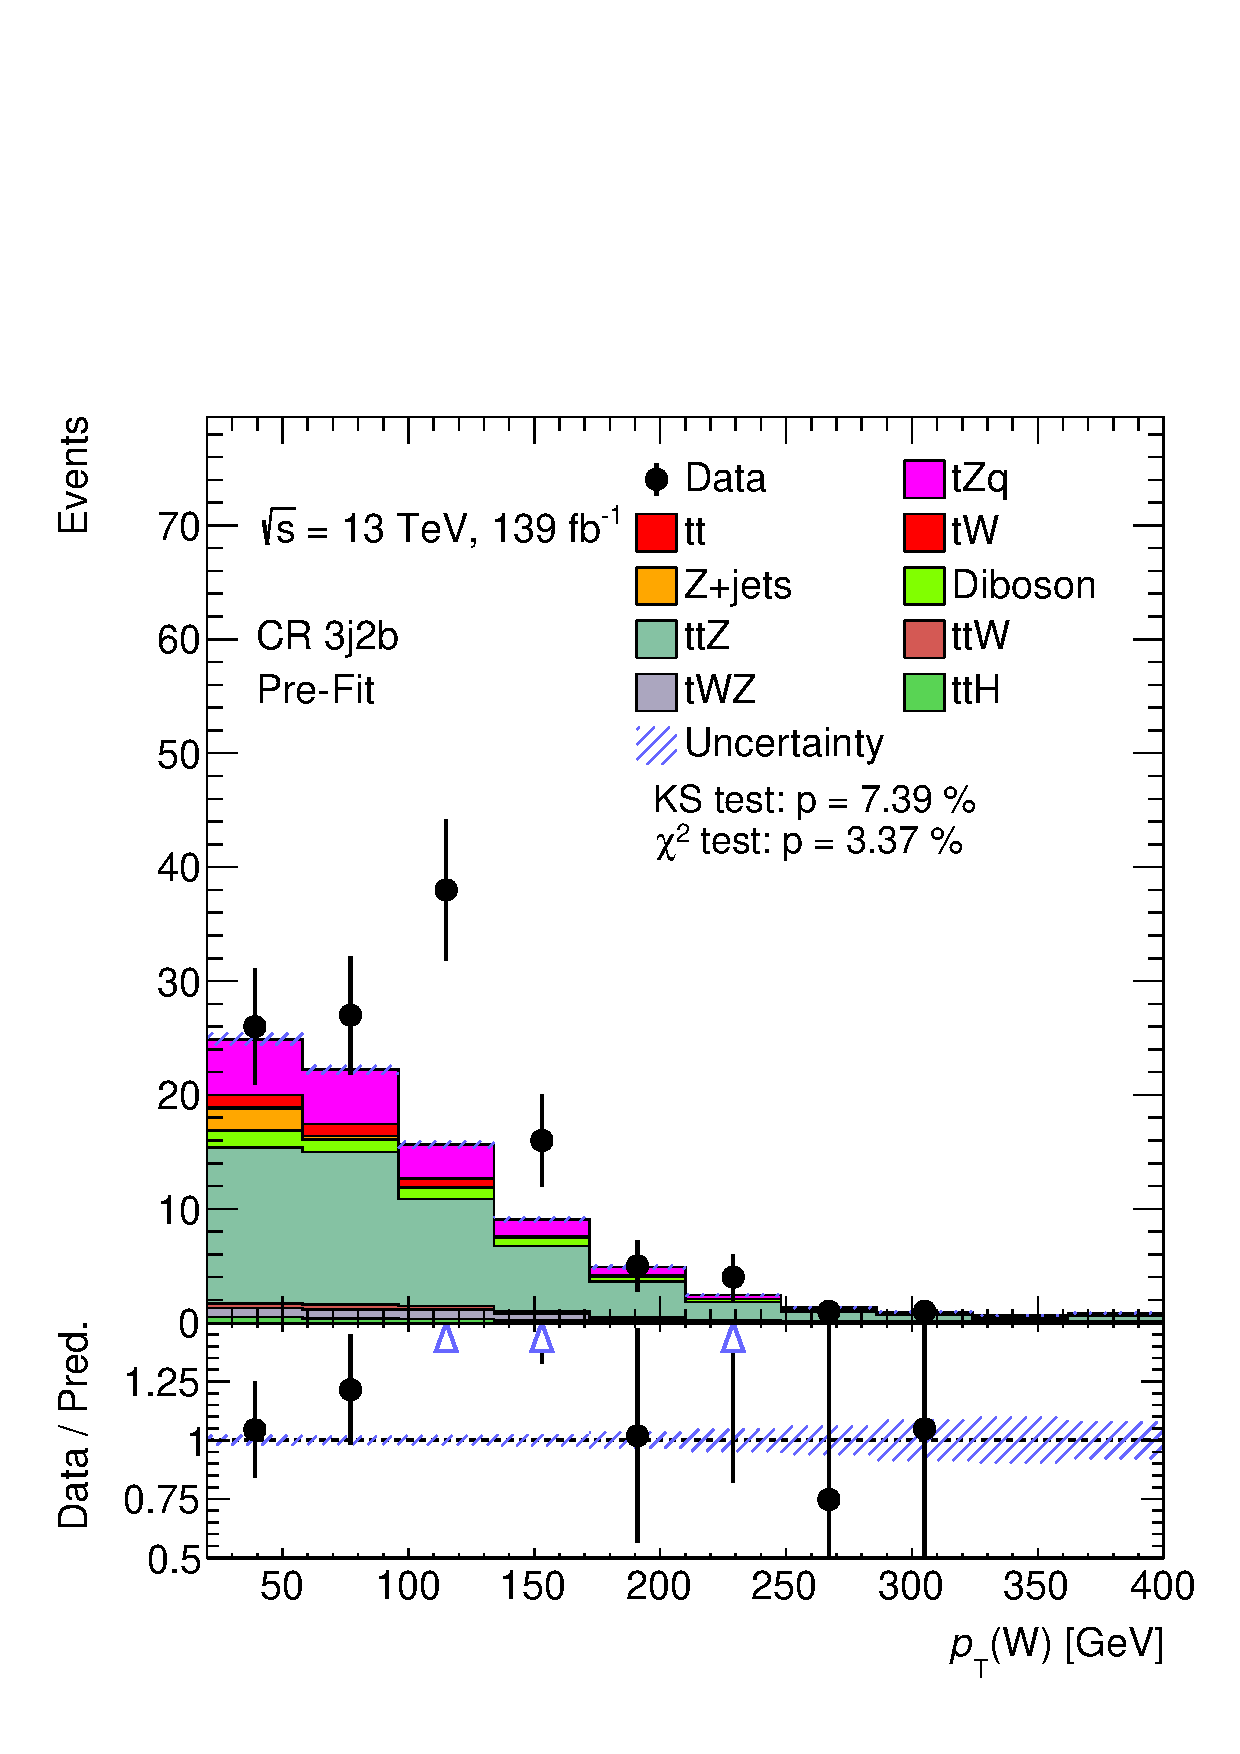
\includegraphics[width=\linewidth]{ubonn-thesis/Chapters/Chapters_06/Figure/Input_distribution/CR_3j2b_W_pt.pdf} 
  \end{subfigure}%%
  \newline
  \begin{subfigure}[b]{0.33\linewidth}
    \centering
    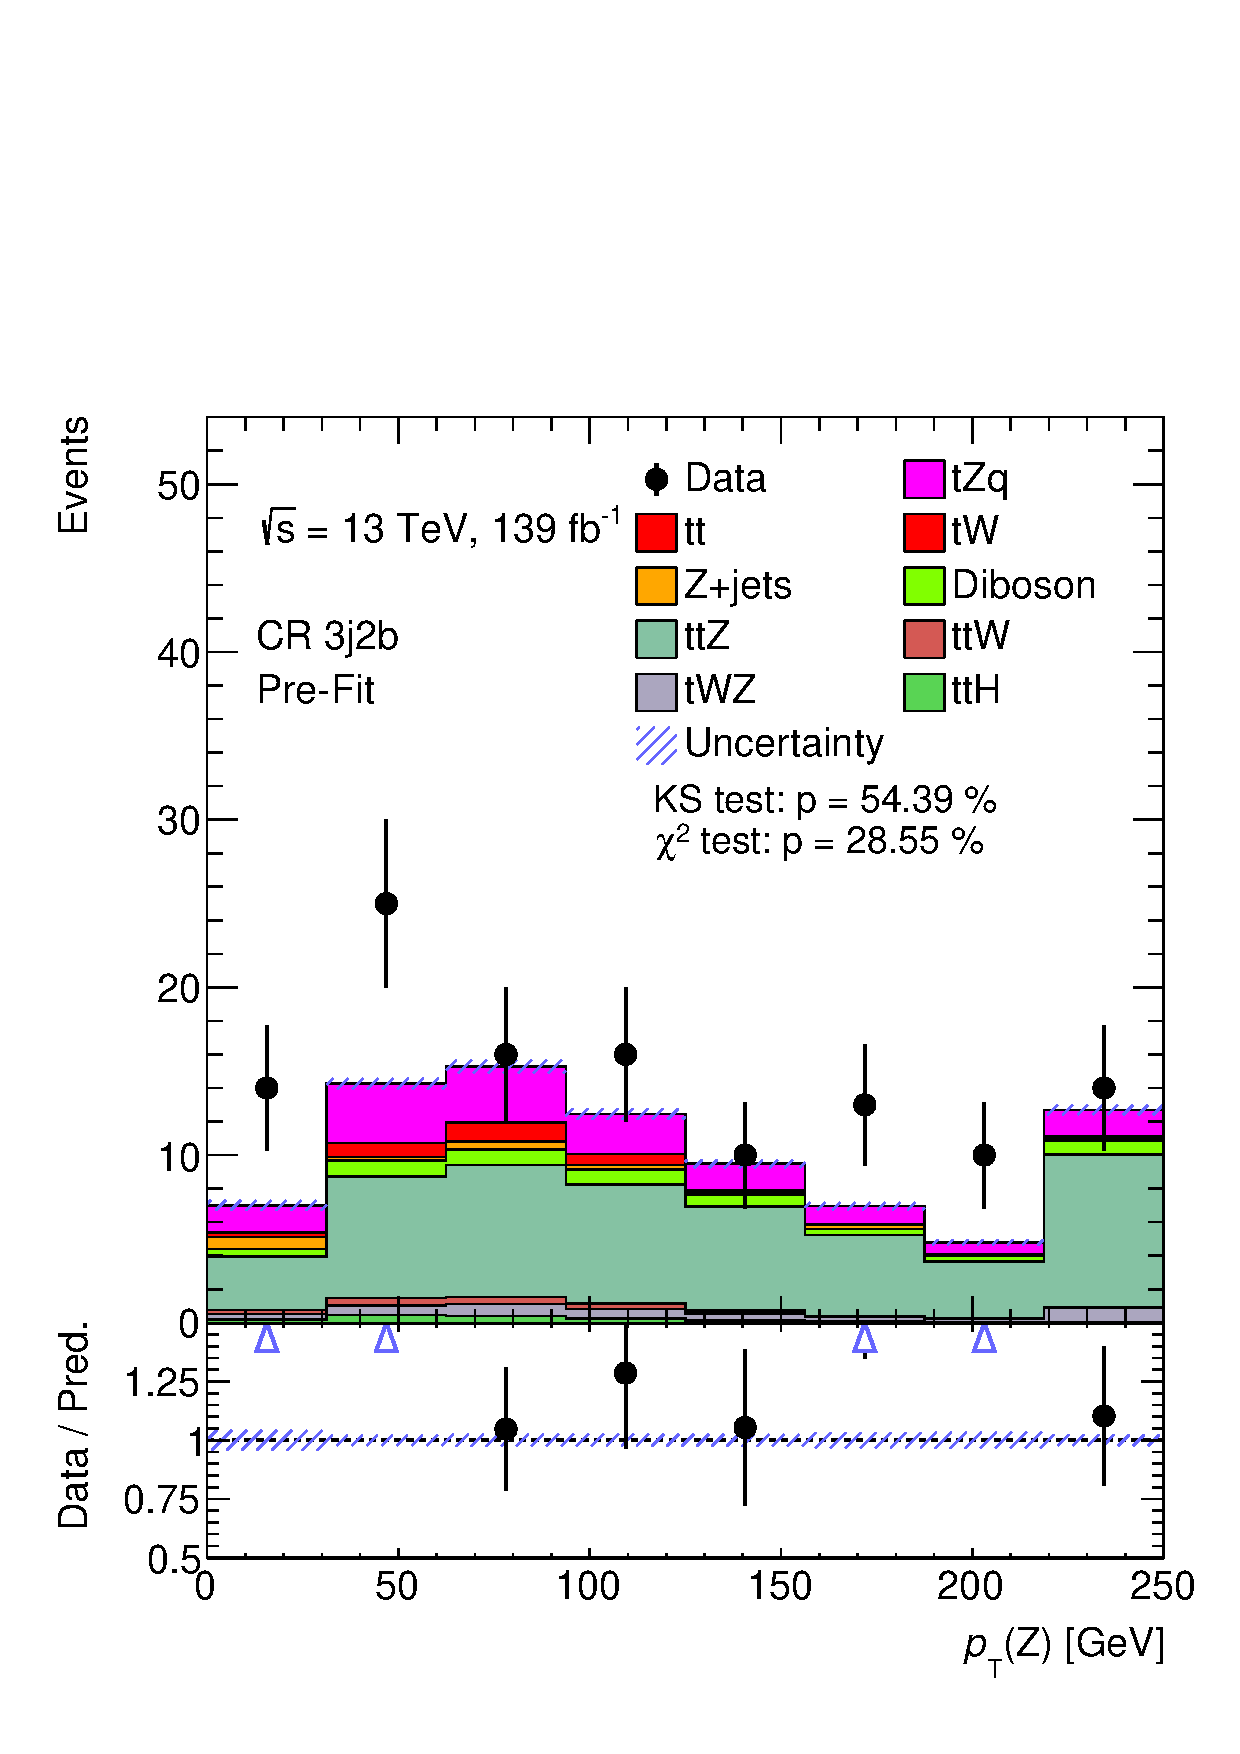
\includegraphics[width=\linewidth]{ubonn-thesis/Chapters/Chapters_06/Figure/Input_distribution/CR_3j2b_Z_pt.pdf} 
  \end{subfigure} 
  \begin{subfigure}[b]{0.33\linewidth}
    \centering
    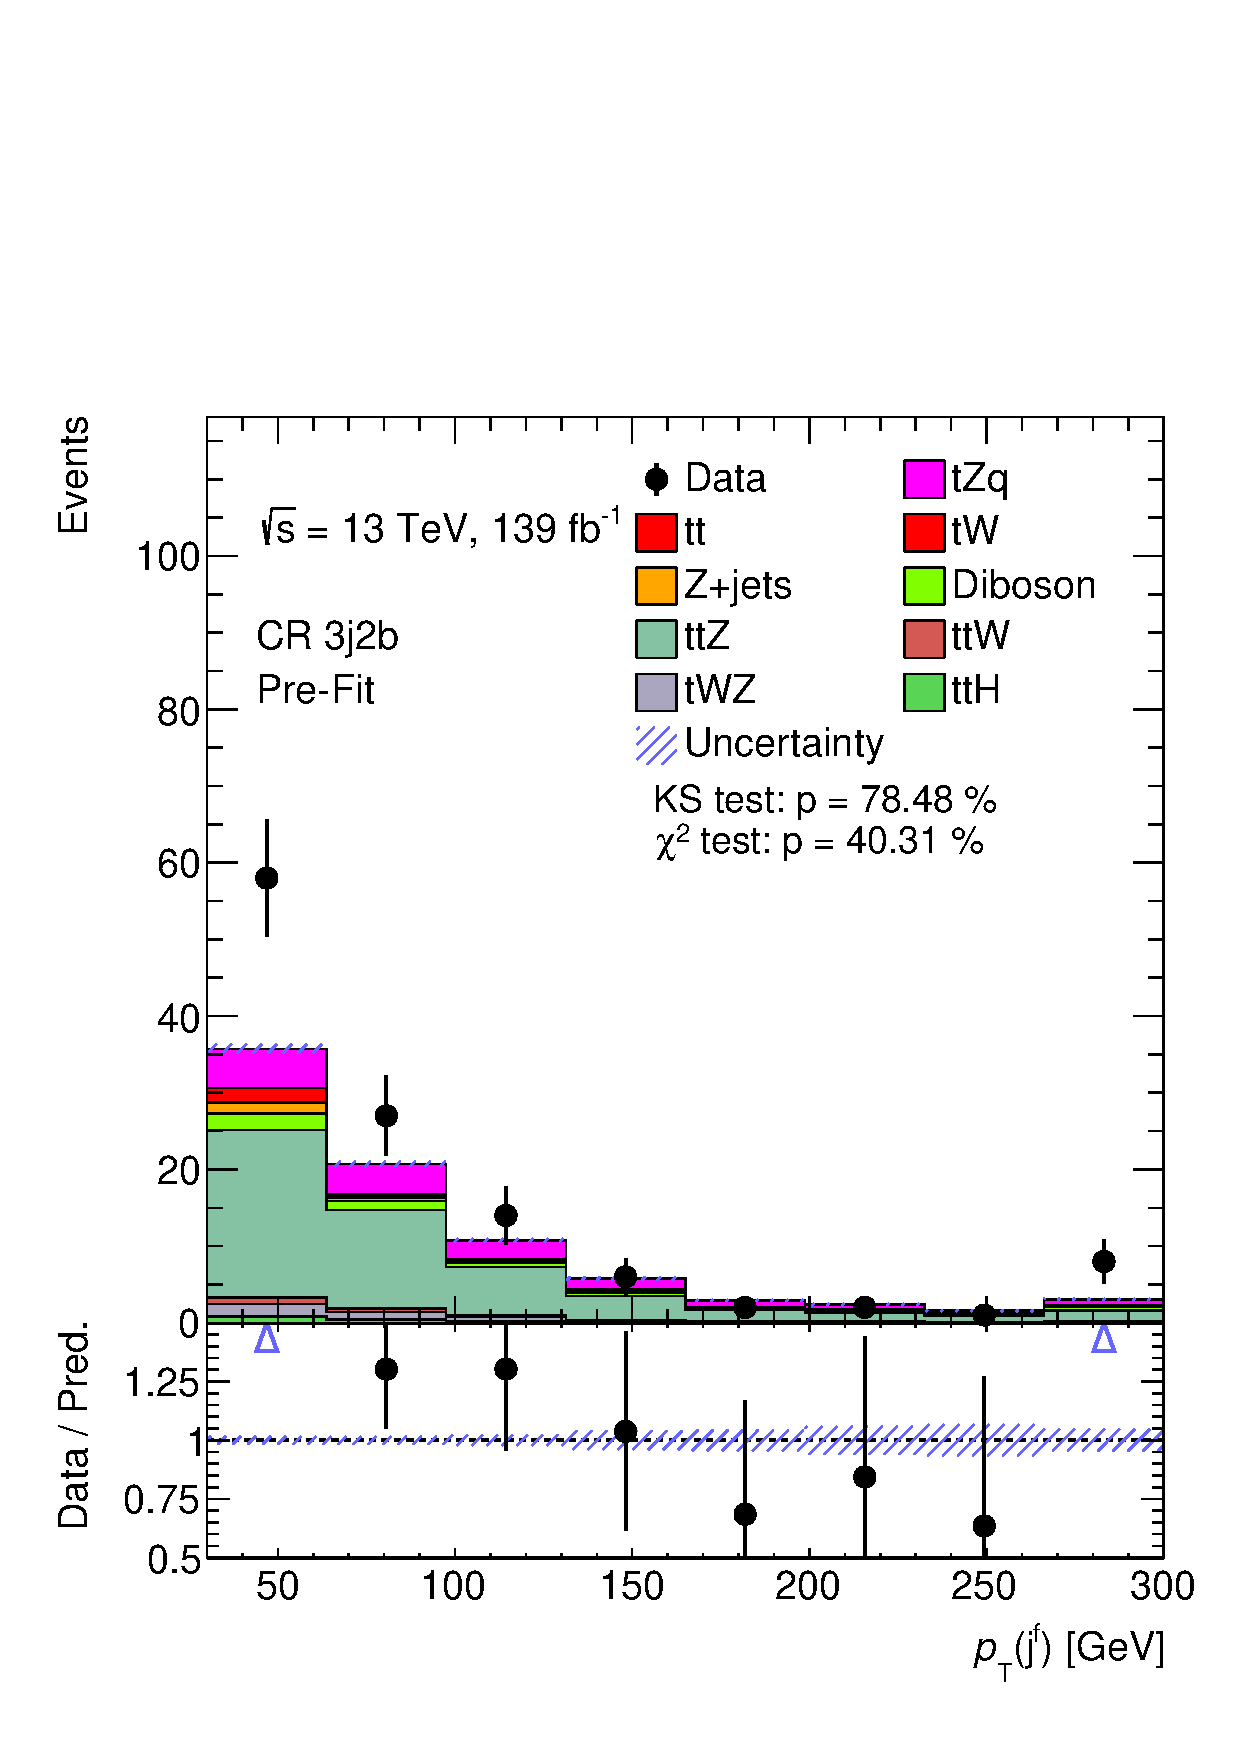
\includegraphics[width=\linewidth]{ubonn-thesis/Chapters/Chapters_06/Figure/Input_distribution/CR_3j2b_forwardjet_pt.pdf} 
  \end{subfigure}%% 
  \begin{subfigure}[b]{0.33\linewidth}
    \centering
    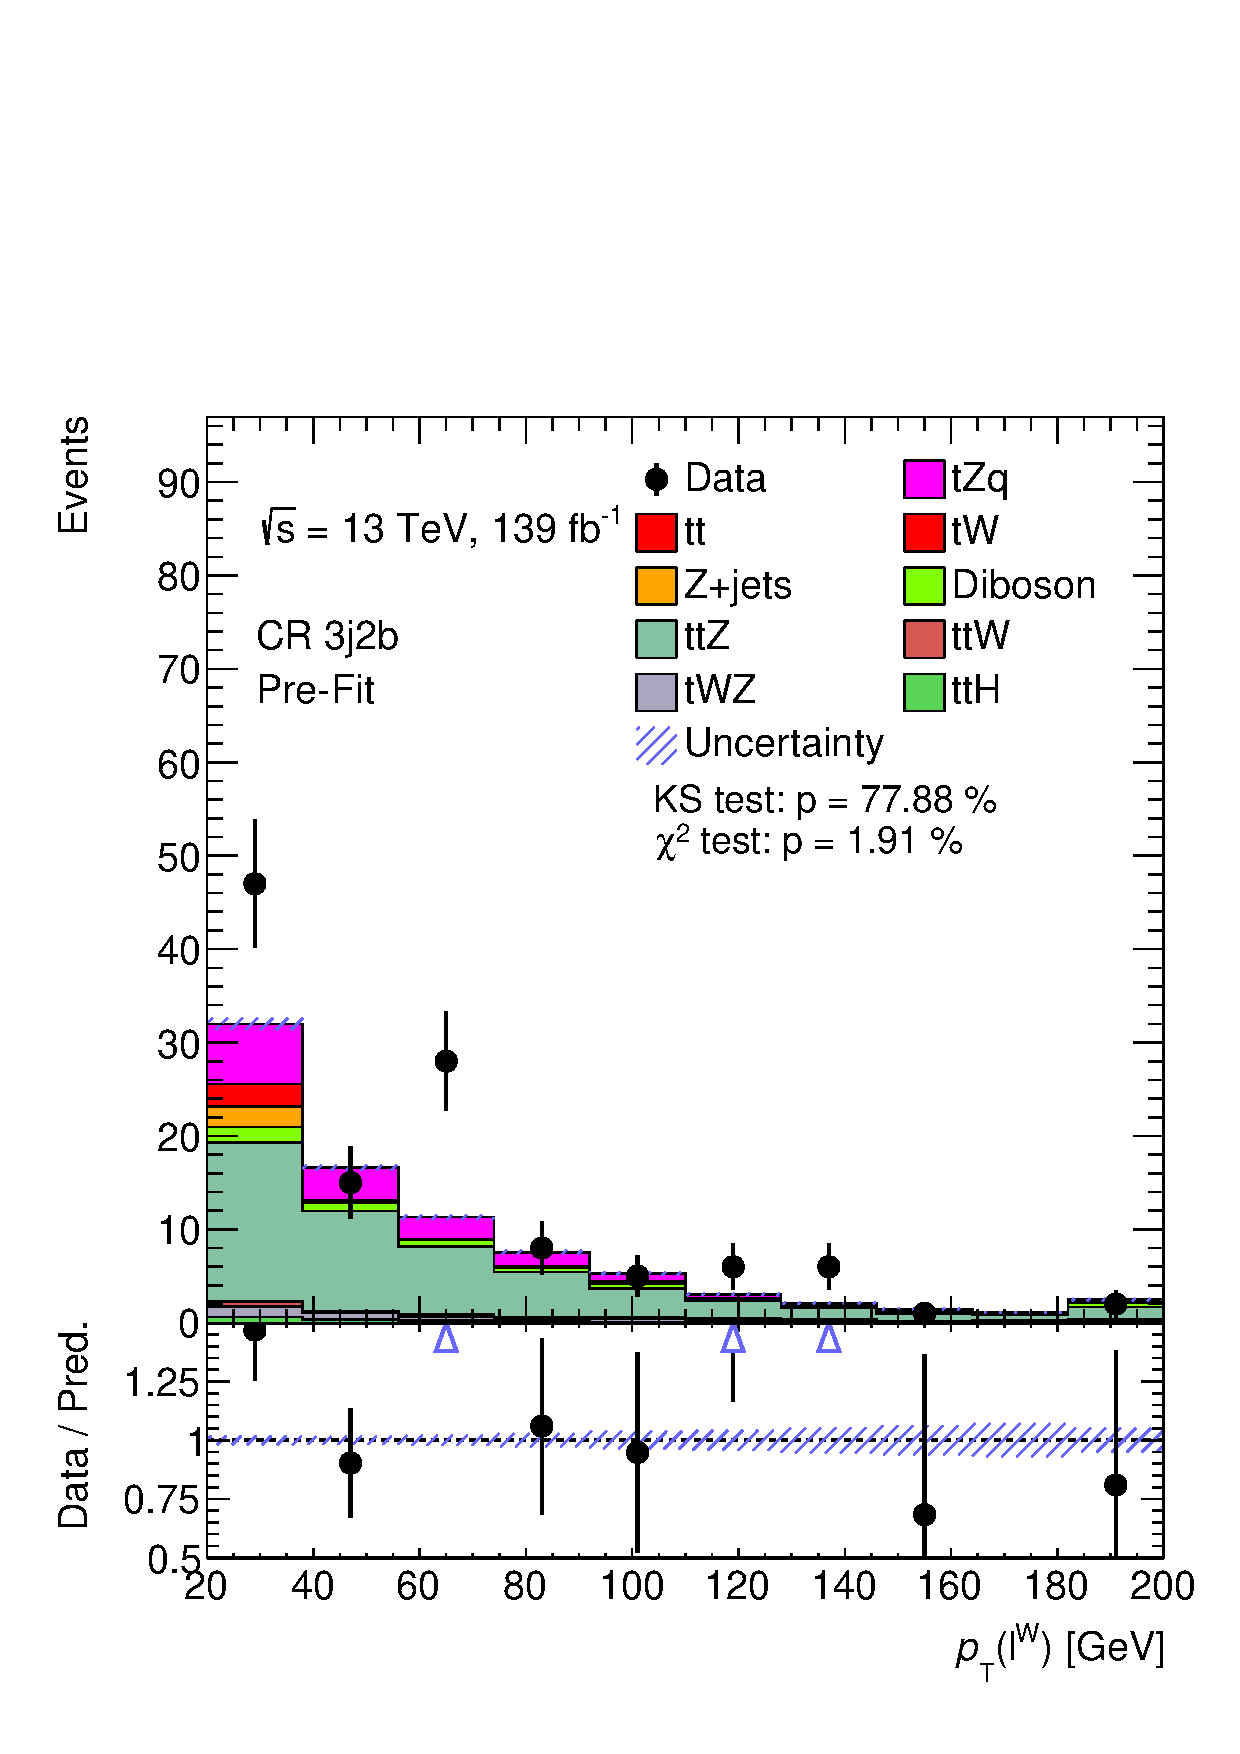
\includegraphics[width=\linewidth]{ubonn-thesis/Chapters/Chapters_06/Figure/Input_distribution/CR_3j2b_lepW_pt.pdf} 
  \end{subfigure} 
  \newline
  \begin{subfigure}[b]{0.33\linewidth}
    \centering
    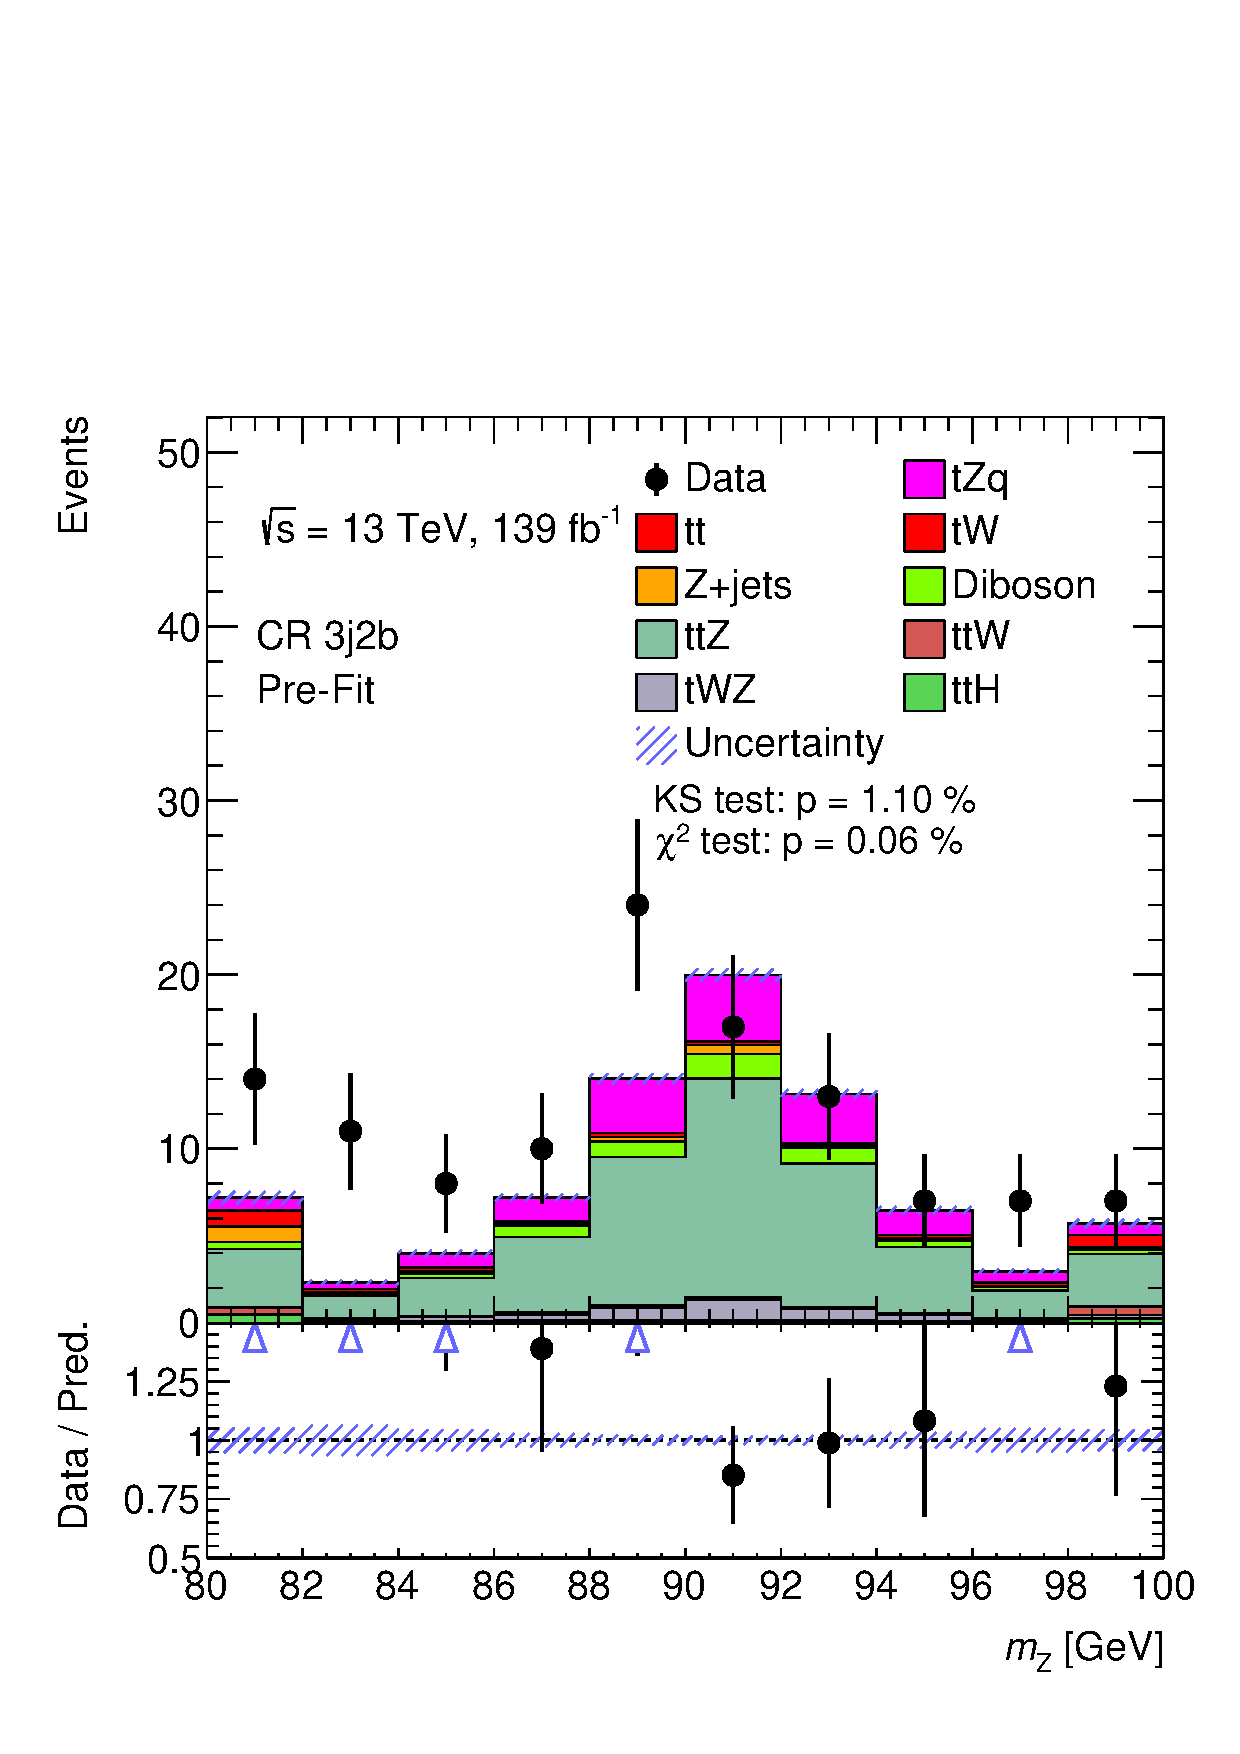
\includegraphics[width=\linewidth]{ubonn-thesis/Chapters/Chapters_06/Figure/Input_distribution/CR_3j2b_MZ.pdf} 
  \end{subfigure}%%
  \begin{subfigure}[b]{0.33\linewidth}
    \centering
    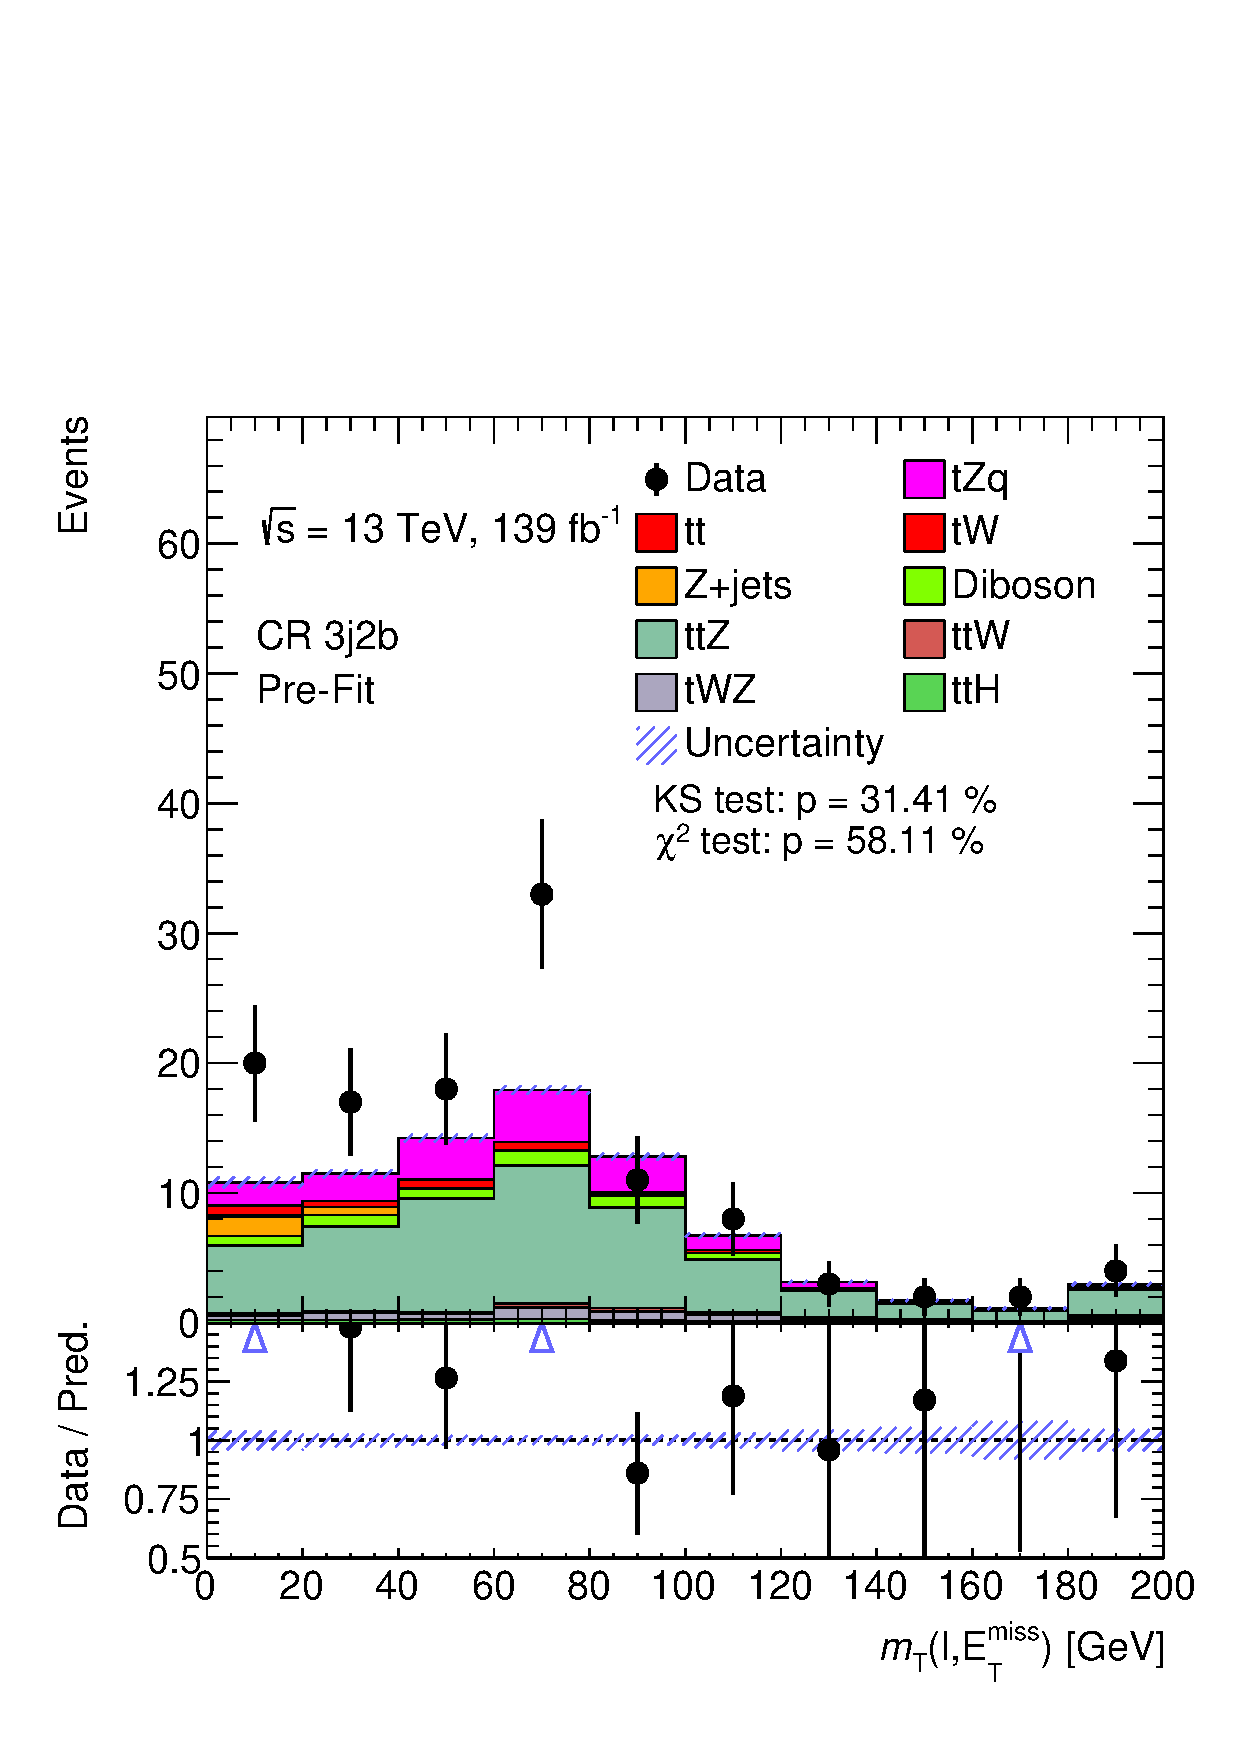
\includegraphics[width=\linewidth]{ubonn-thesis/Chapters/Chapters_06/Figure/Input_distribution/CR_3j2b_mtW.pdf} 
  \end{subfigure}
  \begin{subfigure}[b]{0.33\linewidth}
    \centering
    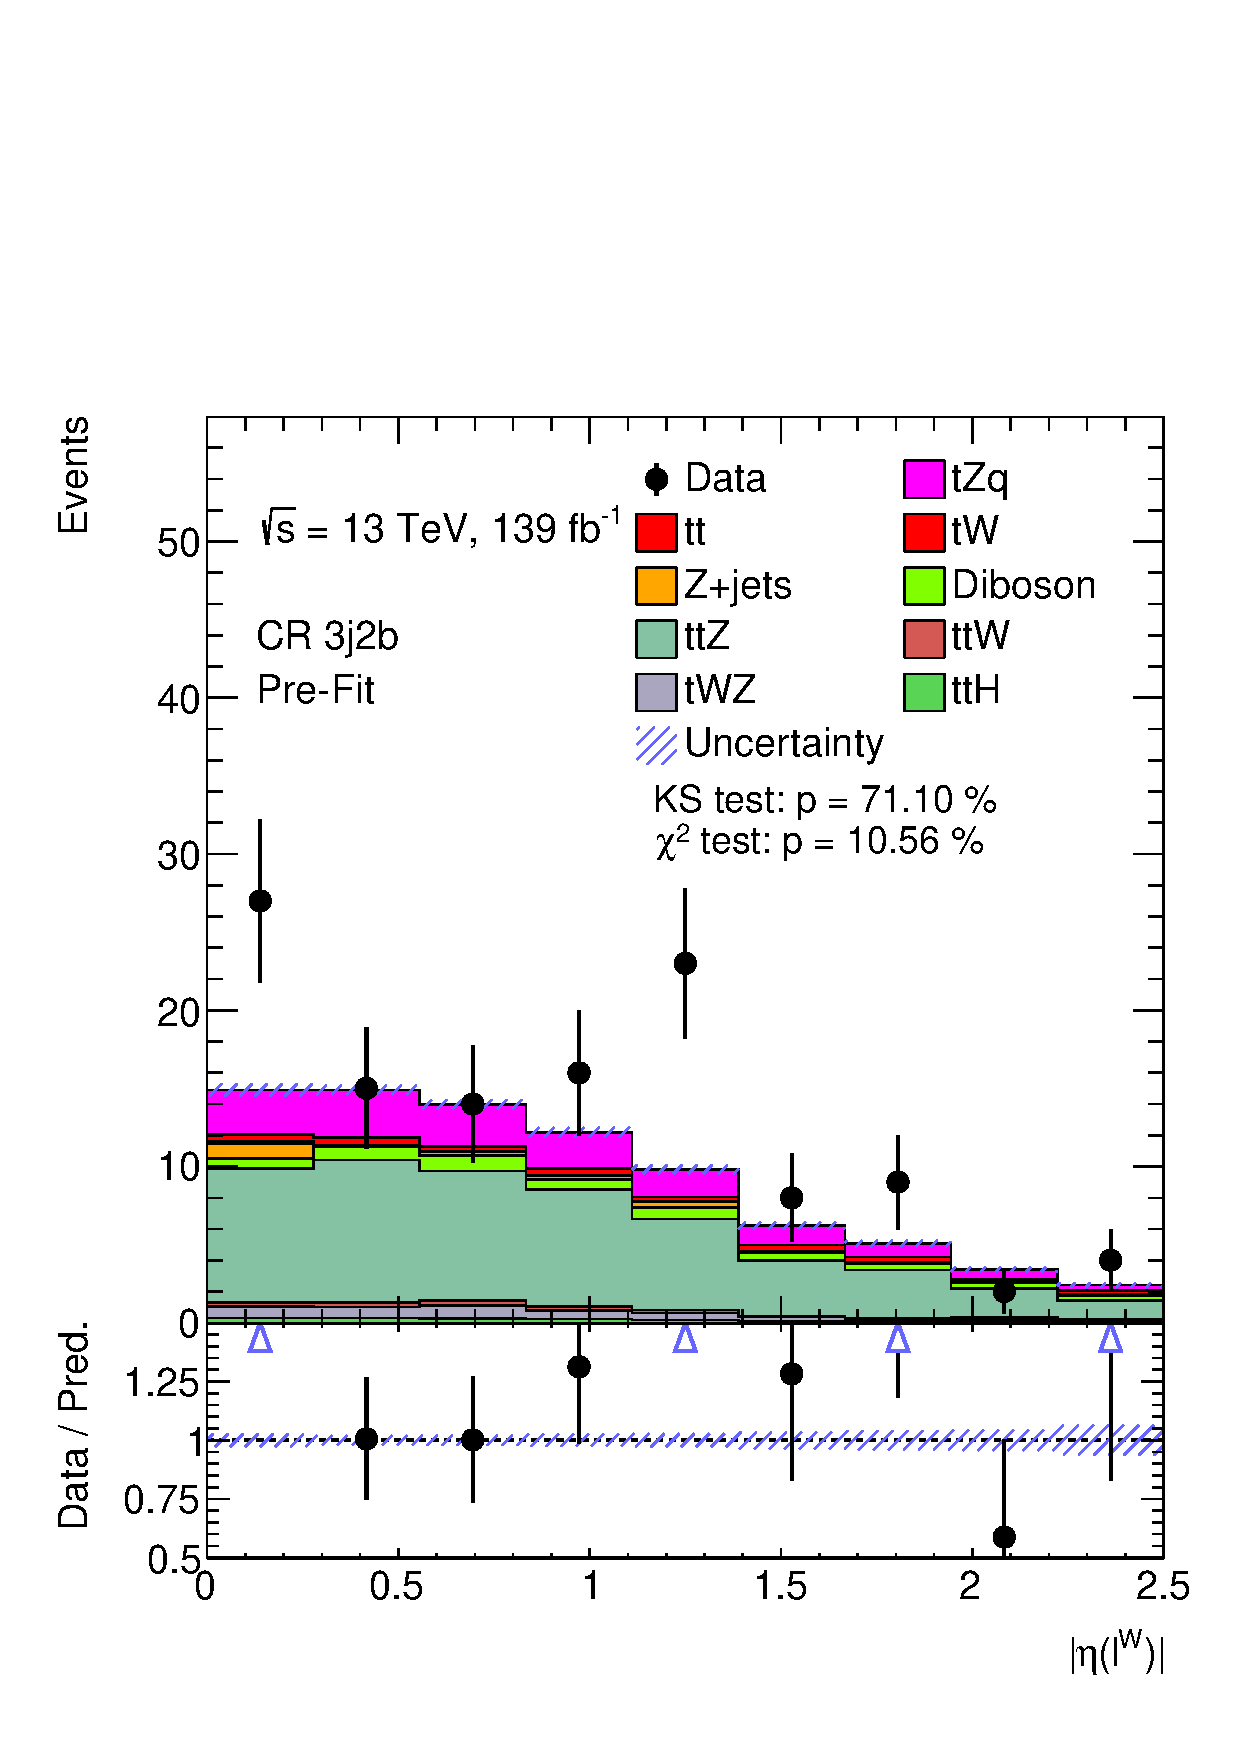
\includegraphics[width=\linewidth]{ubonn-thesis/Chapters/Chapters_06/Figure/Input_distribution/CR_3j2b_lepW_eta.pdf} 
  \end{subfigure} 
  
  \caption{ Stacked kinematic plots of neural-network training variables of the CR 3j2b, in order of significance. Both signal and backgrounds are normalised to the expected number of events before the fit. The uncertainty band includes statistical uncertainties for signal and backgrounds }
  \label{fig_control1} 
  \end{figure}


\begin{figure}
    \begin{subfigure}[b]{0.32\linewidth}
    \centering
    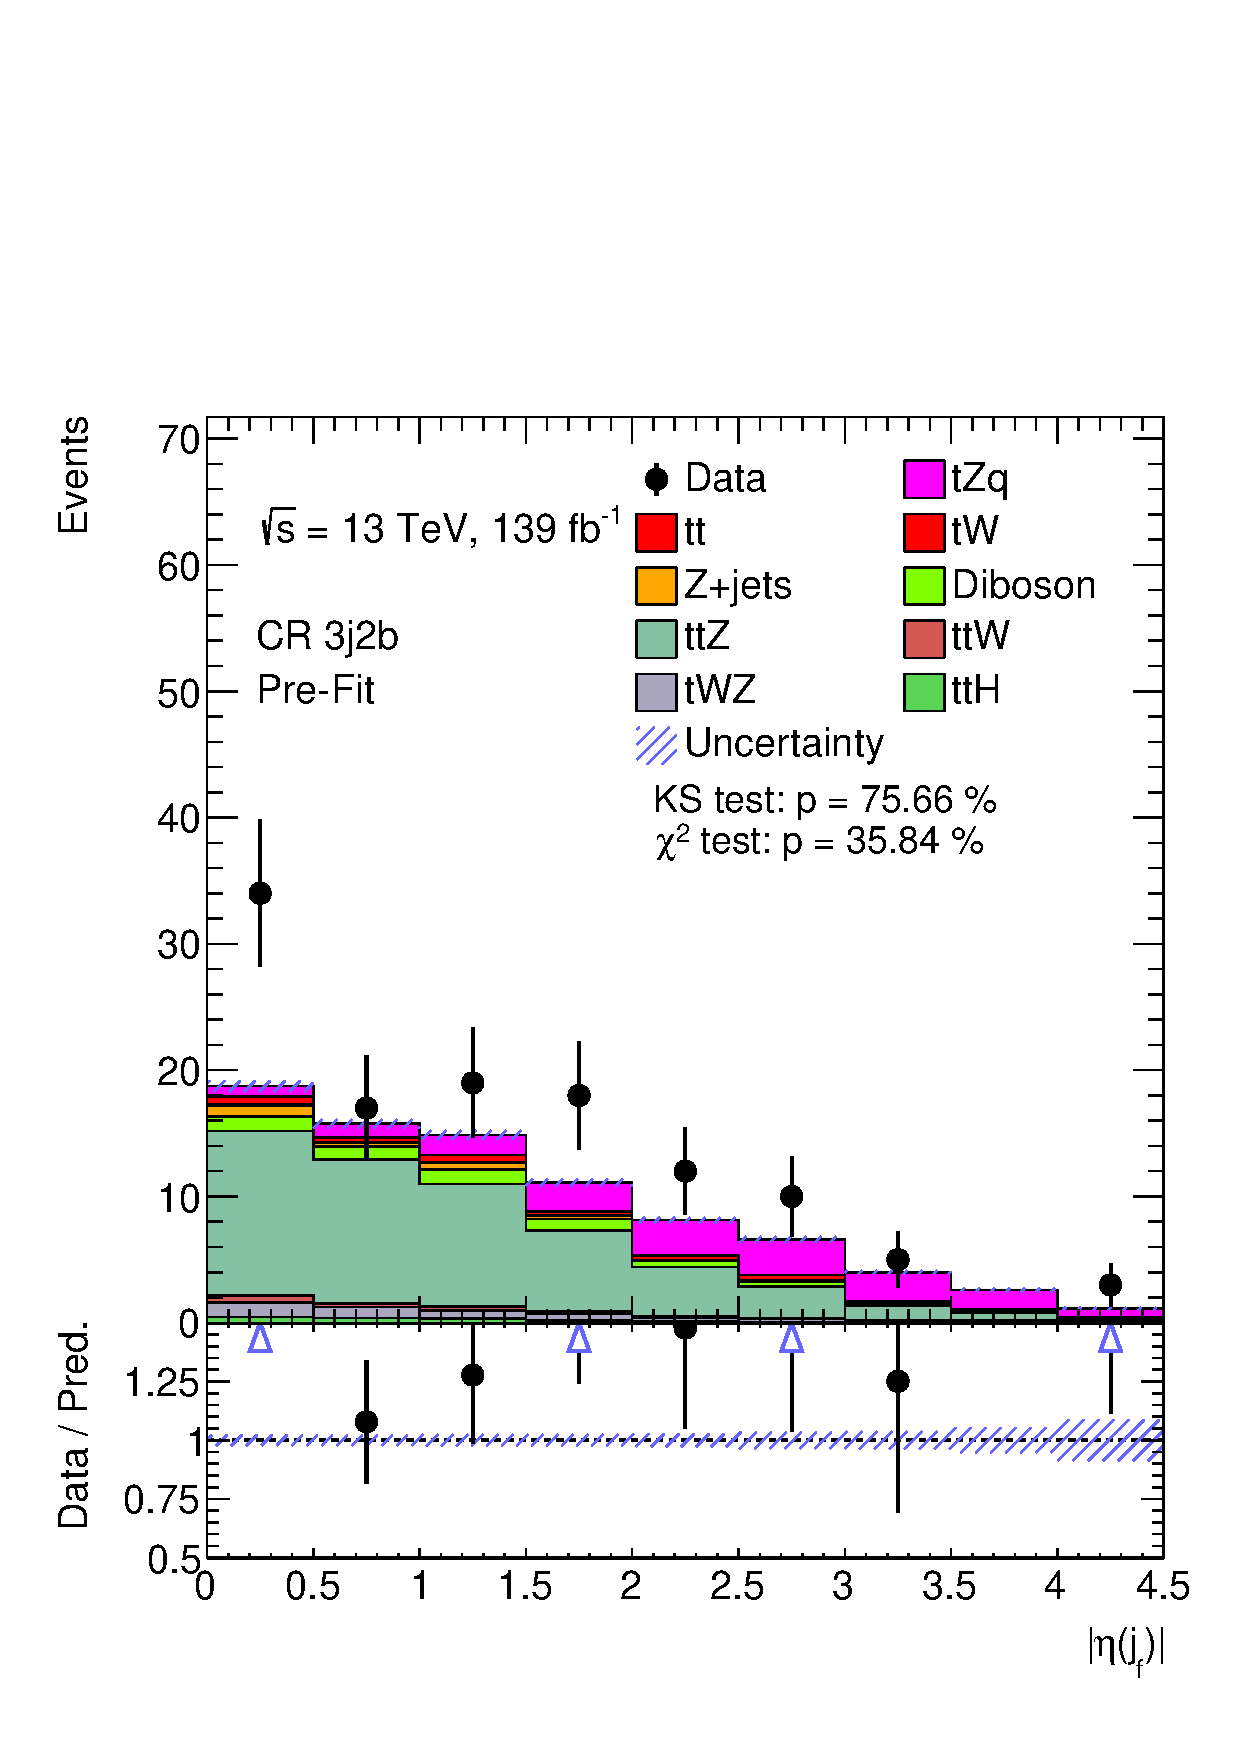
\includegraphics[width=\linewidth]{ubonn-thesis/Chapters/Chapters_06/Figure/Input_distribution/CR_3j2b_forwardjet_eta.pdf} 
  \end{subfigure}%%
  \begin{subfigure}[b]{0.32\linewidth}
    \centering
    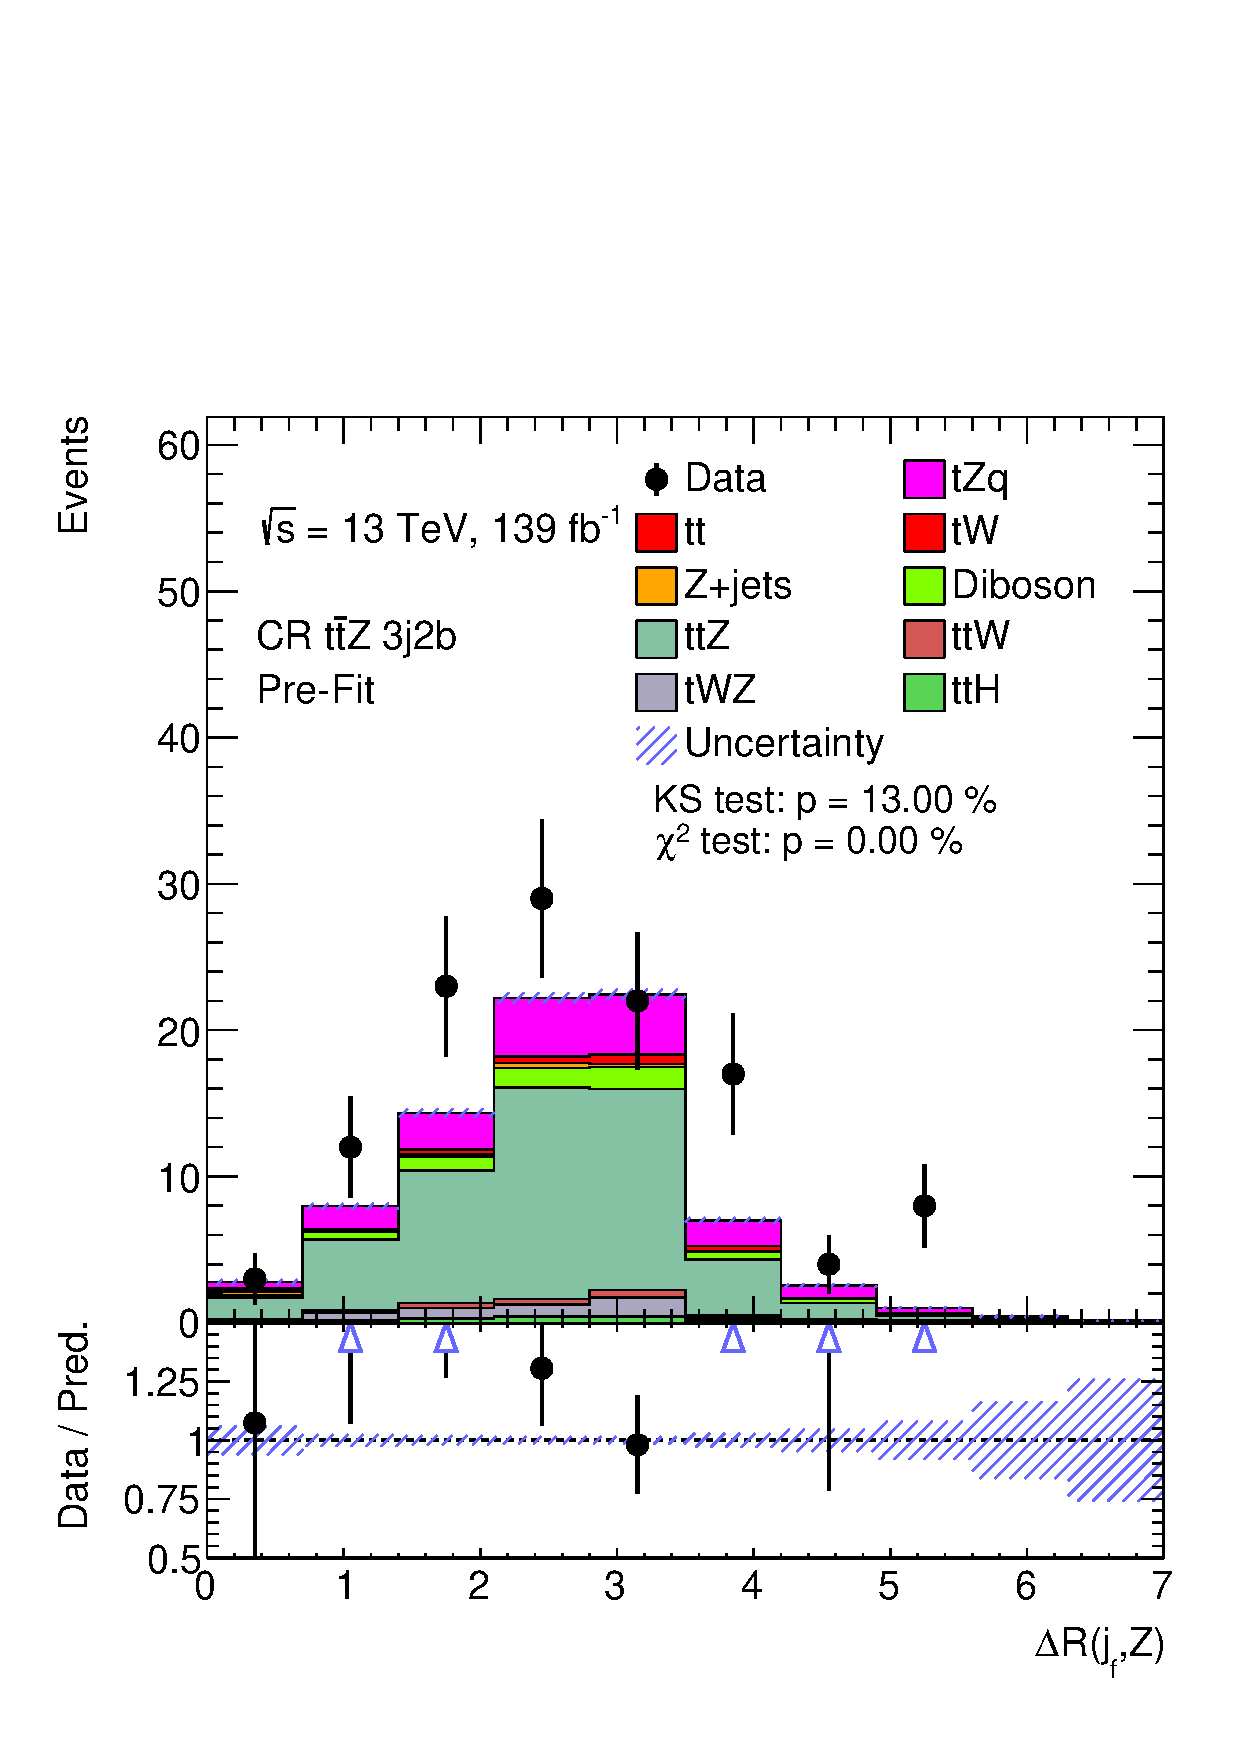
\includegraphics[width=\linewidth]{ubonn-thesis/Chapters/Chapters_06/Figure/Input_distribution/CR_3j2b_dR_jf_Z.pdf} 
  \end{subfigure}
  \begin{subfigure}[b]{0.32\linewidth}
    \centering
    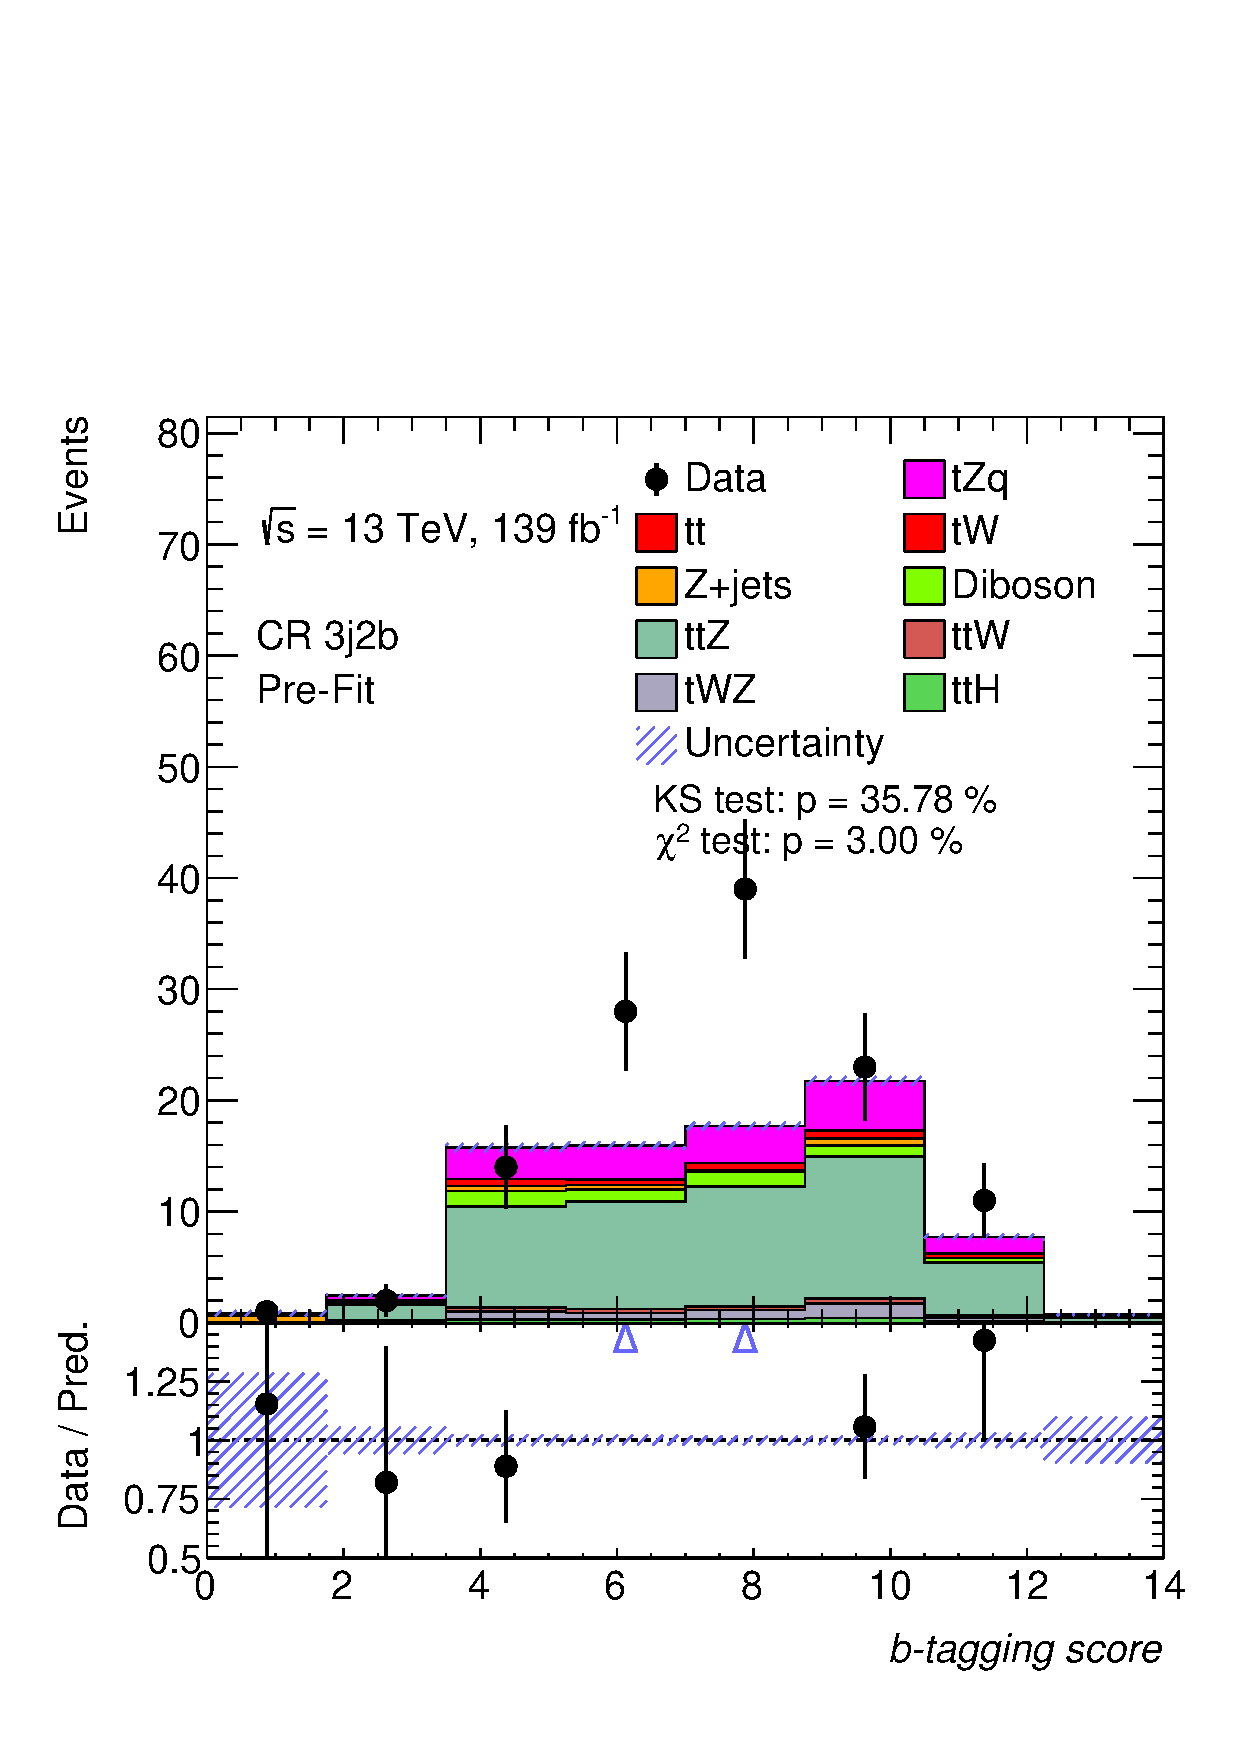
\includegraphics[width=\linewidth]{ubonn-thesis/Chapters/Chapters_06/Figure/Input_distribution/CR_3j2b_btag.pdf} 
  \end{subfigure} 
  \newline
  \centering
  \begin{subfigure}[b]{0.32\linewidth}
    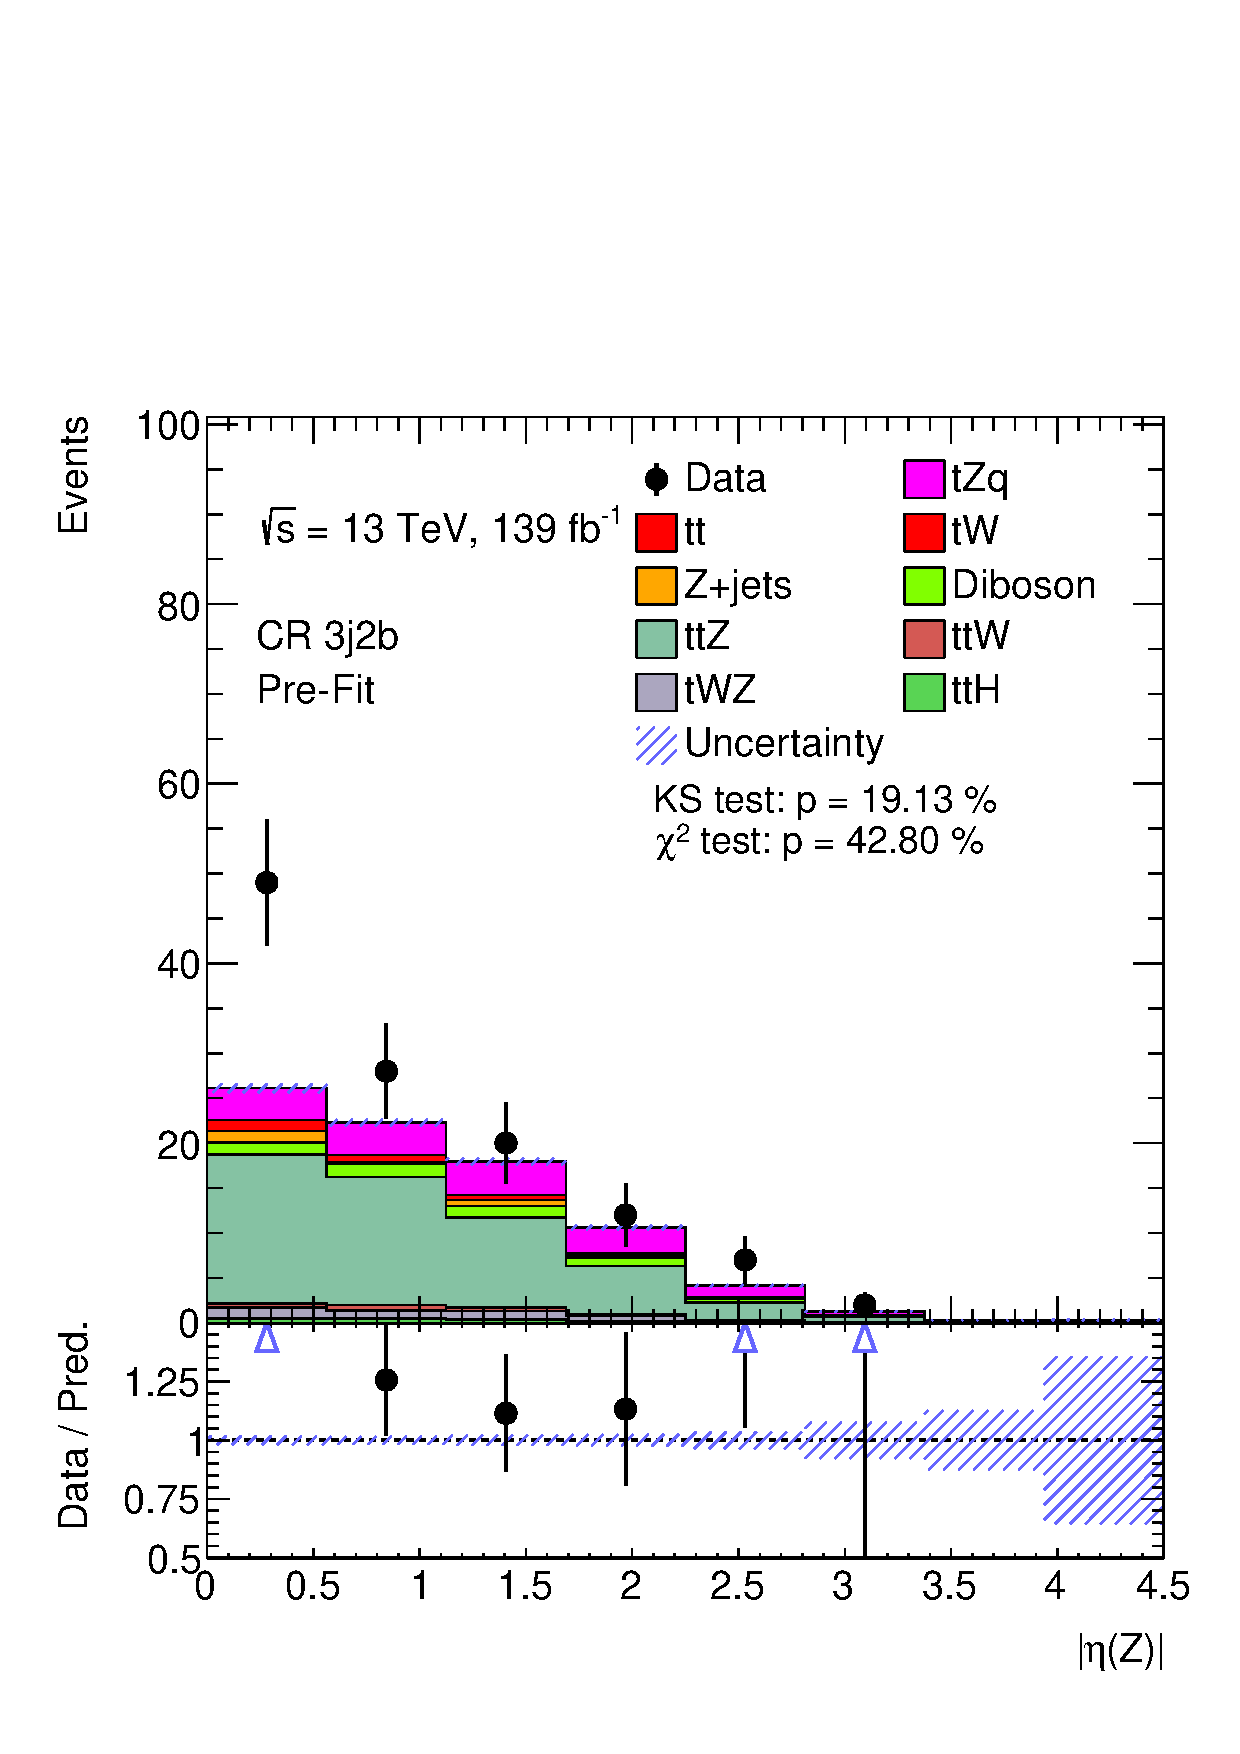
\includegraphics[width=\linewidth]{ubonn-thesis/Chapters/Chapters_06/Figure/Input_distribution/CR_3j2b_Z_eta.pdf} 
  \end{subfigure}%% 
  \hspace*{0.3cm}
  \centering
  \begin{subfigure}[b]{0.32\linewidth}
    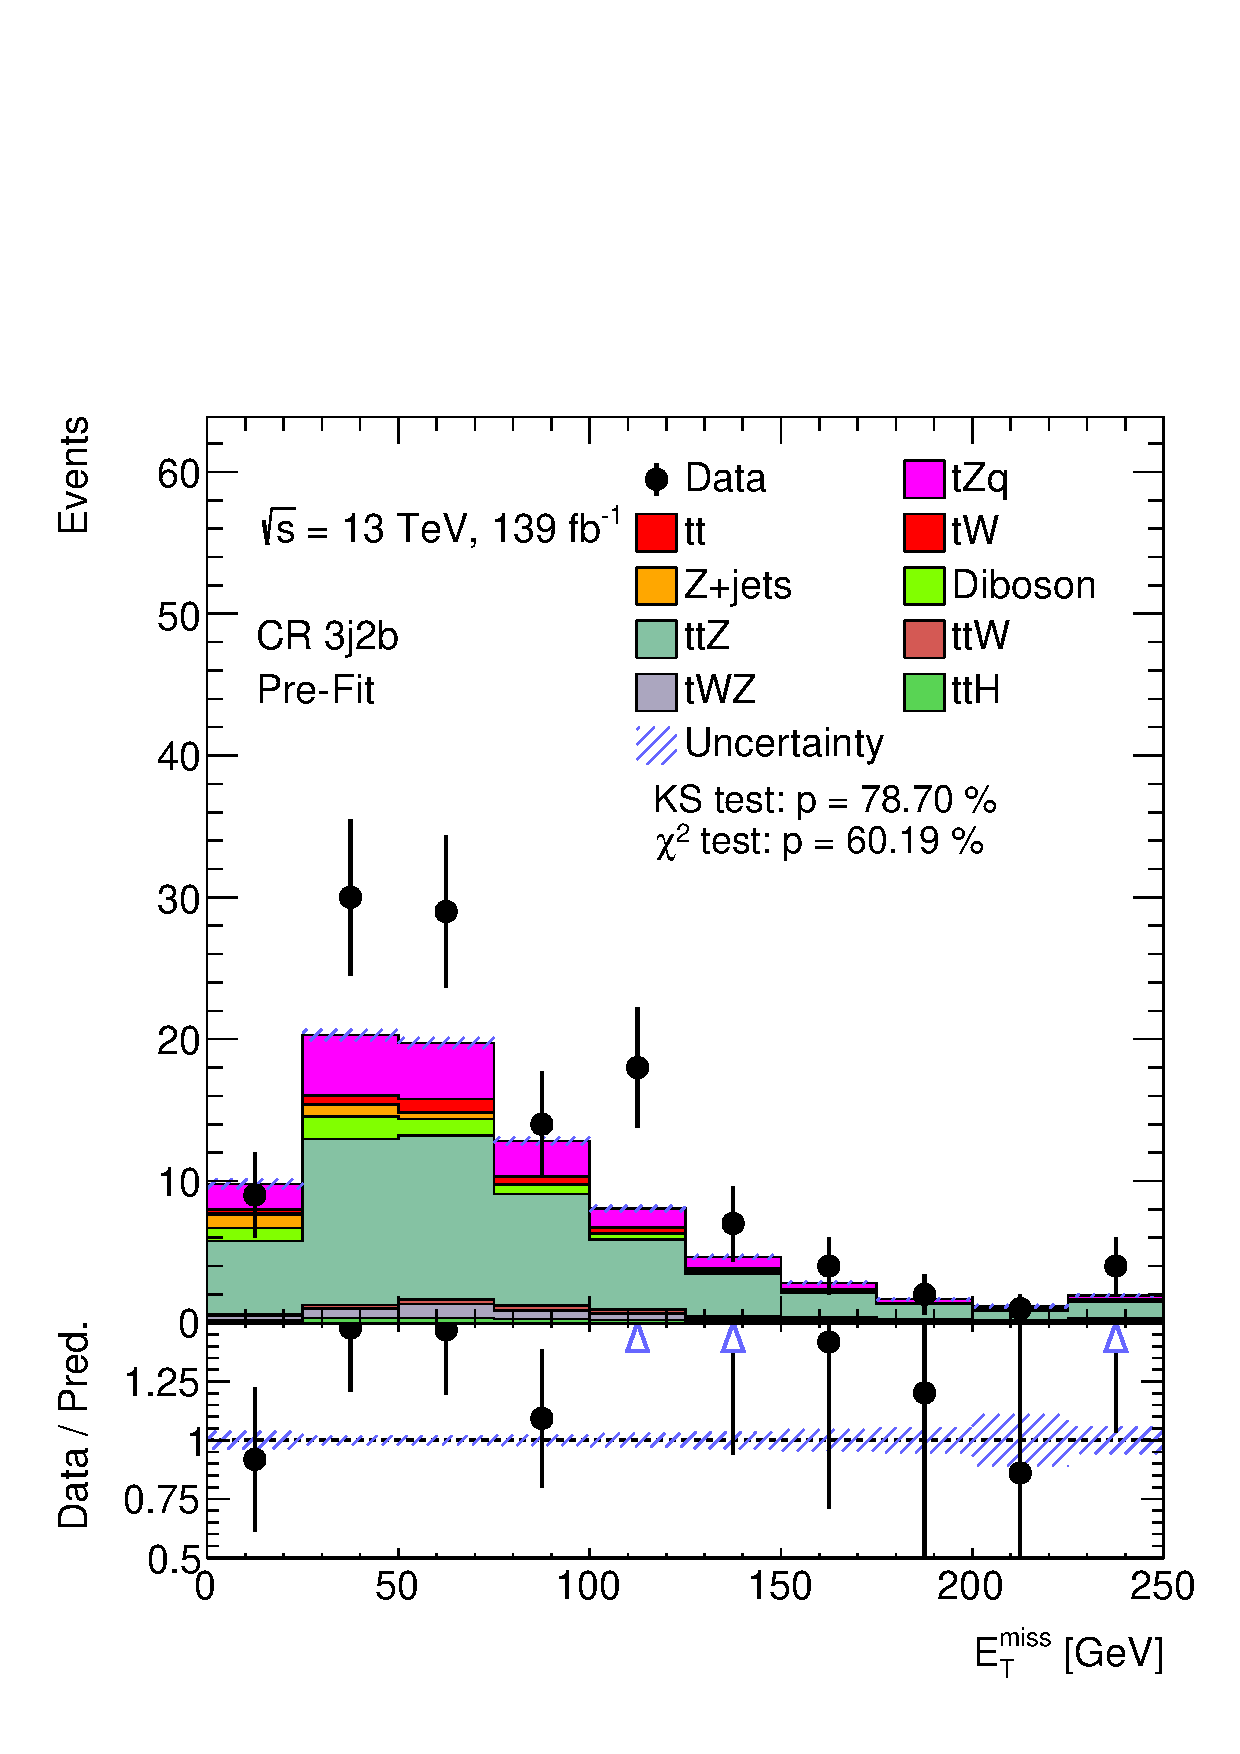
\includegraphics[width=\linewidth]{ubonn-thesis/Chapters/Chapters_06/Figure/Input_distribution/CR_3j2b_MissEt.pdf} 
  \end{subfigure} 
  \caption{Stacked kinematic plots of neural-network training variables of the CR 3j2b, in order of significance. Both signal and backgrounds are normalised to the expected number of events before the fit. The uncertainty band includes statistical uncertainties for signal and backgrounds}
  \label{fig_control2} 
\end{figure}
%% delta R and pt of forward jet

%% SR 3j1b
\begin{figure}[!h] 
  \begin{subfigure}[b]{0.32\linewidth}
    \centering
    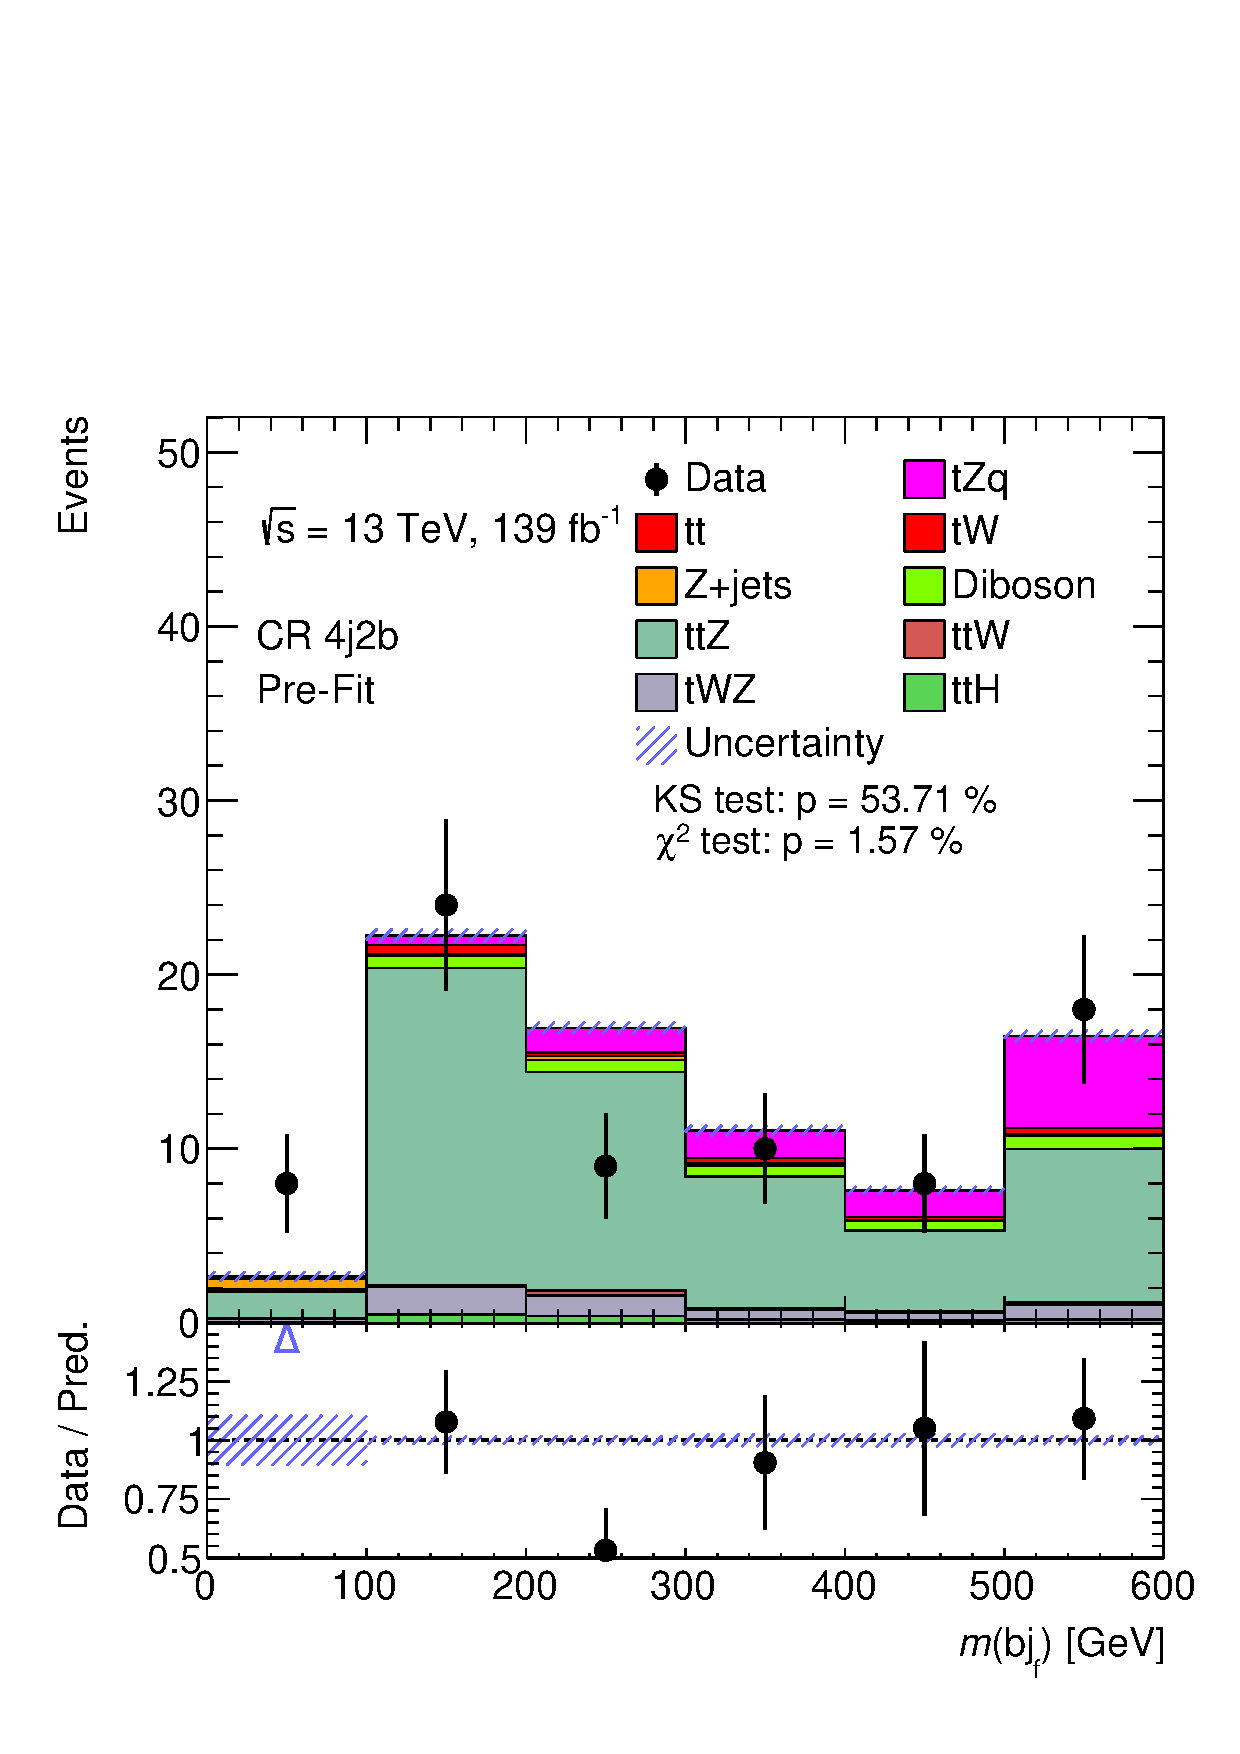
\includegraphics[width=\linewidth]{ubonn-thesis/Chapters/Chapters_06/Figure/Input_distribution/CR_4j2b_M_bj.pdf} 
  \end{subfigure}%% 
  \begin{subfigure}[b]{0.32\linewidth}
    \centering
    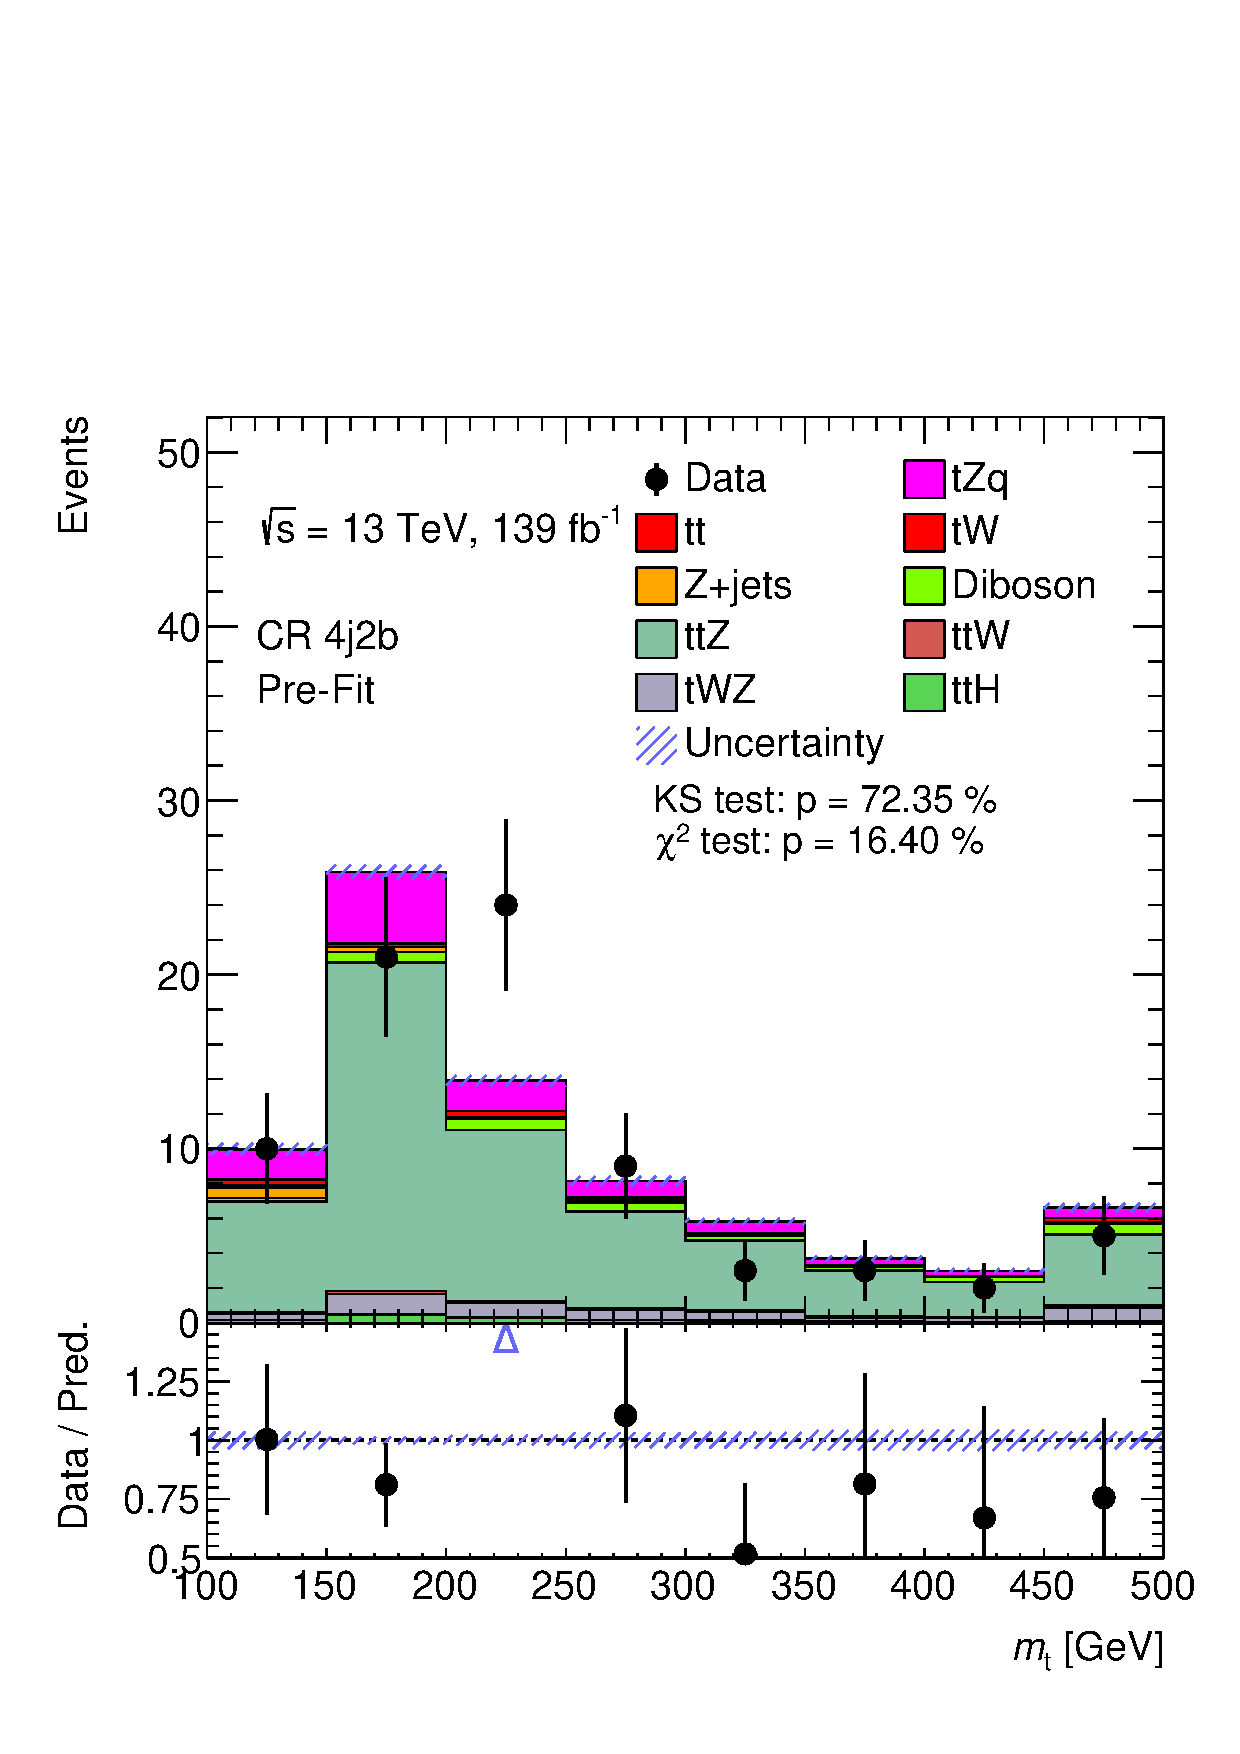
\includegraphics[width=\linewidth]{ubonn-thesis/Chapters/Chapters_06/Figure/Input_distribution/CR_4j2b_Top_mass.pdf} 
  \end{subfigure} 
  \begin{subfigure}[b]{0.32\linewidth}
    \centering
    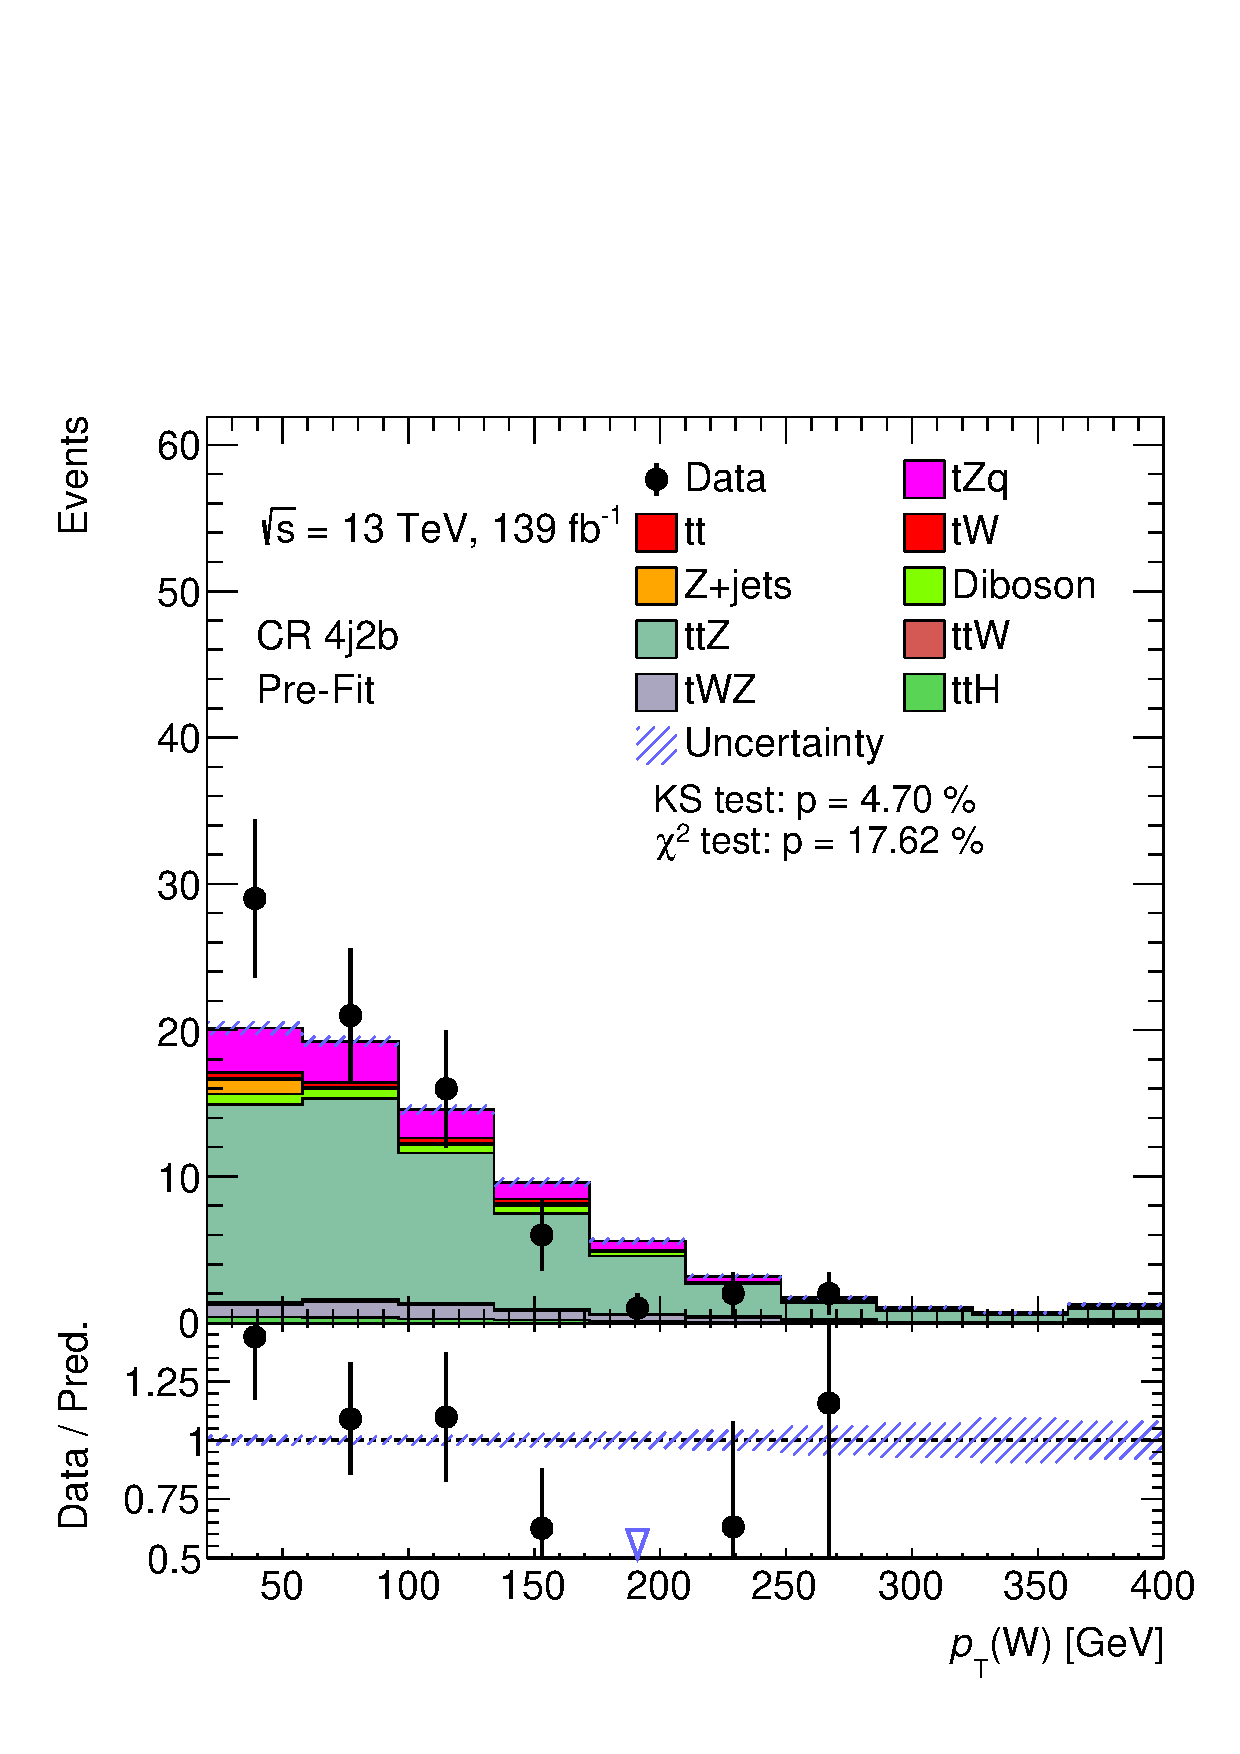
\includegraphics[width=\linewidth]{ubonn-thesis/Chapters/Chapters_06/Figure/Input_distribution/CR_4j2b_W_pt.pdf} 
  \end{subfigure}%%
  \caption{Stacked kinematic plots of neural-network training variables of the CR 4j2b, in order of significance. Both signal and backgrounds are normalised to the expected number of events before the fit. The uncertainty band includes statistical uncertainties for signal and backgrounds}
  \label{fig_control3}
  \end{figure}


\begin{figure}[!h] 
\vspace*{0.4cm}
  \begin{subfigure}[b]{0.33\linewidth}
    \centering
    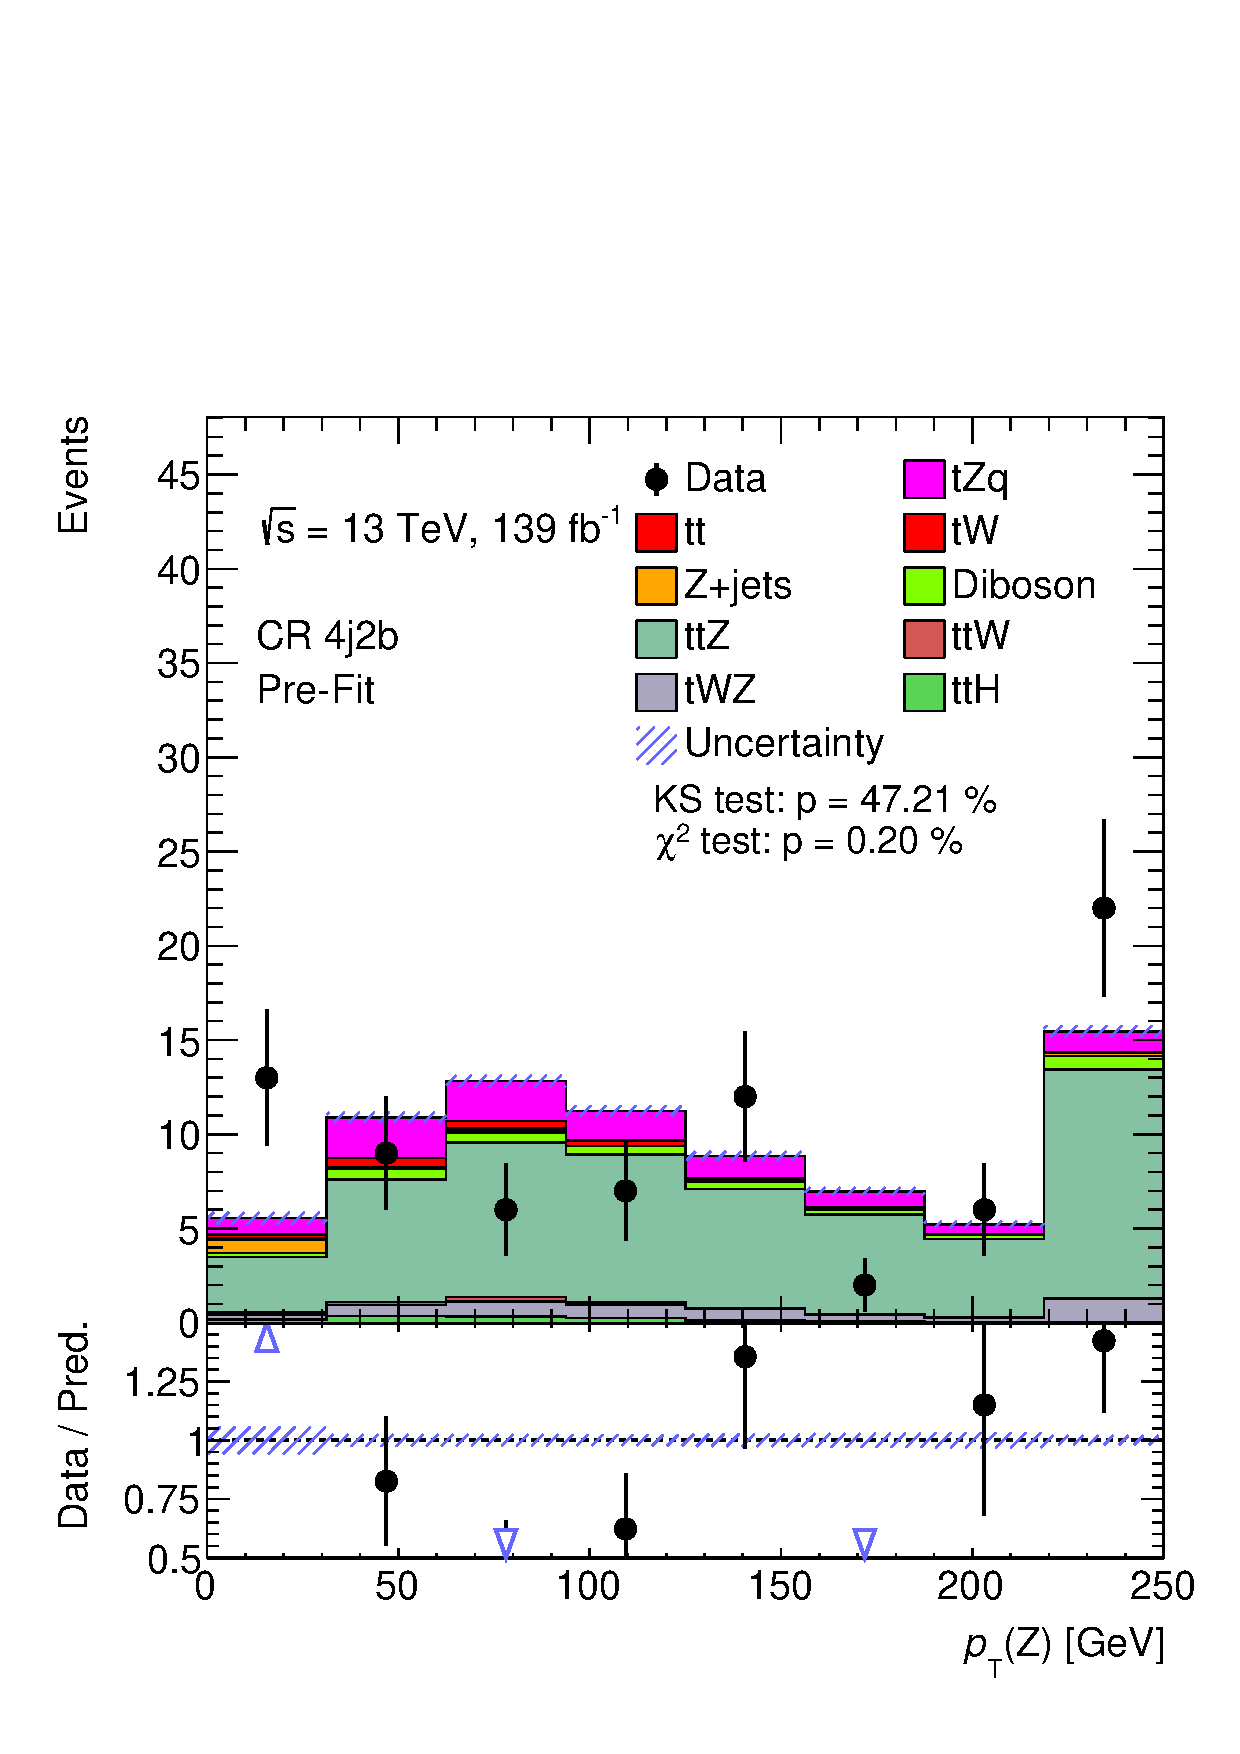
\includegraphics[width=\linewidth]{ubonn-thesis/Chapters/Chapters_06/Figure/Input_distribution/CR_4j2b_Z_pt.pdf} 
  \end{subfigure} 
  \begin{subfigure}[b]{0.33\linewidth}
    \centering
    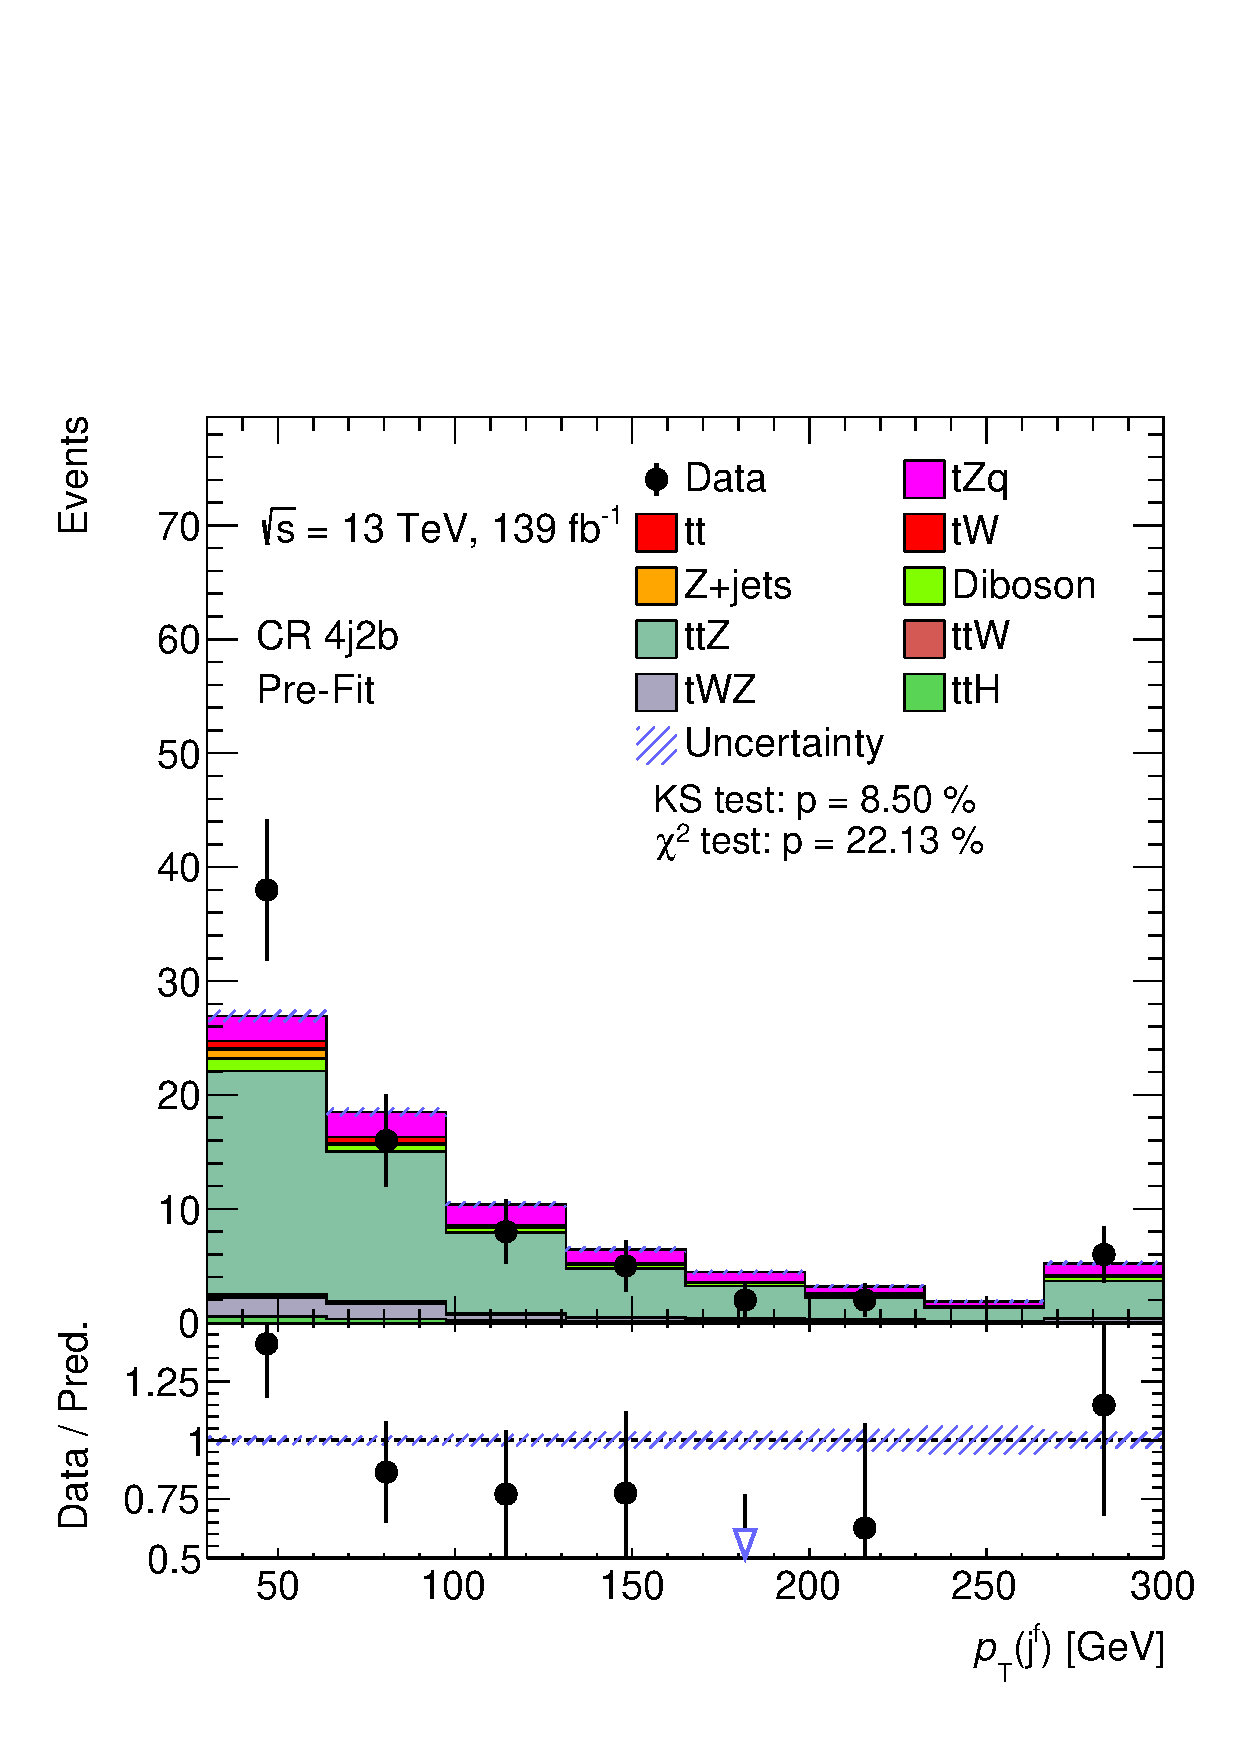
\includegraphics[width=\linewidth]{ubonn-thesis/Chapters/Chapters_06/Figure/Input_distribution/CR_4j2b_forwardjet_pt.pdf} 
  \end{subfigure}%% 
  \begin{subfigure}[b]{0.33\linewidth}
    \centering
    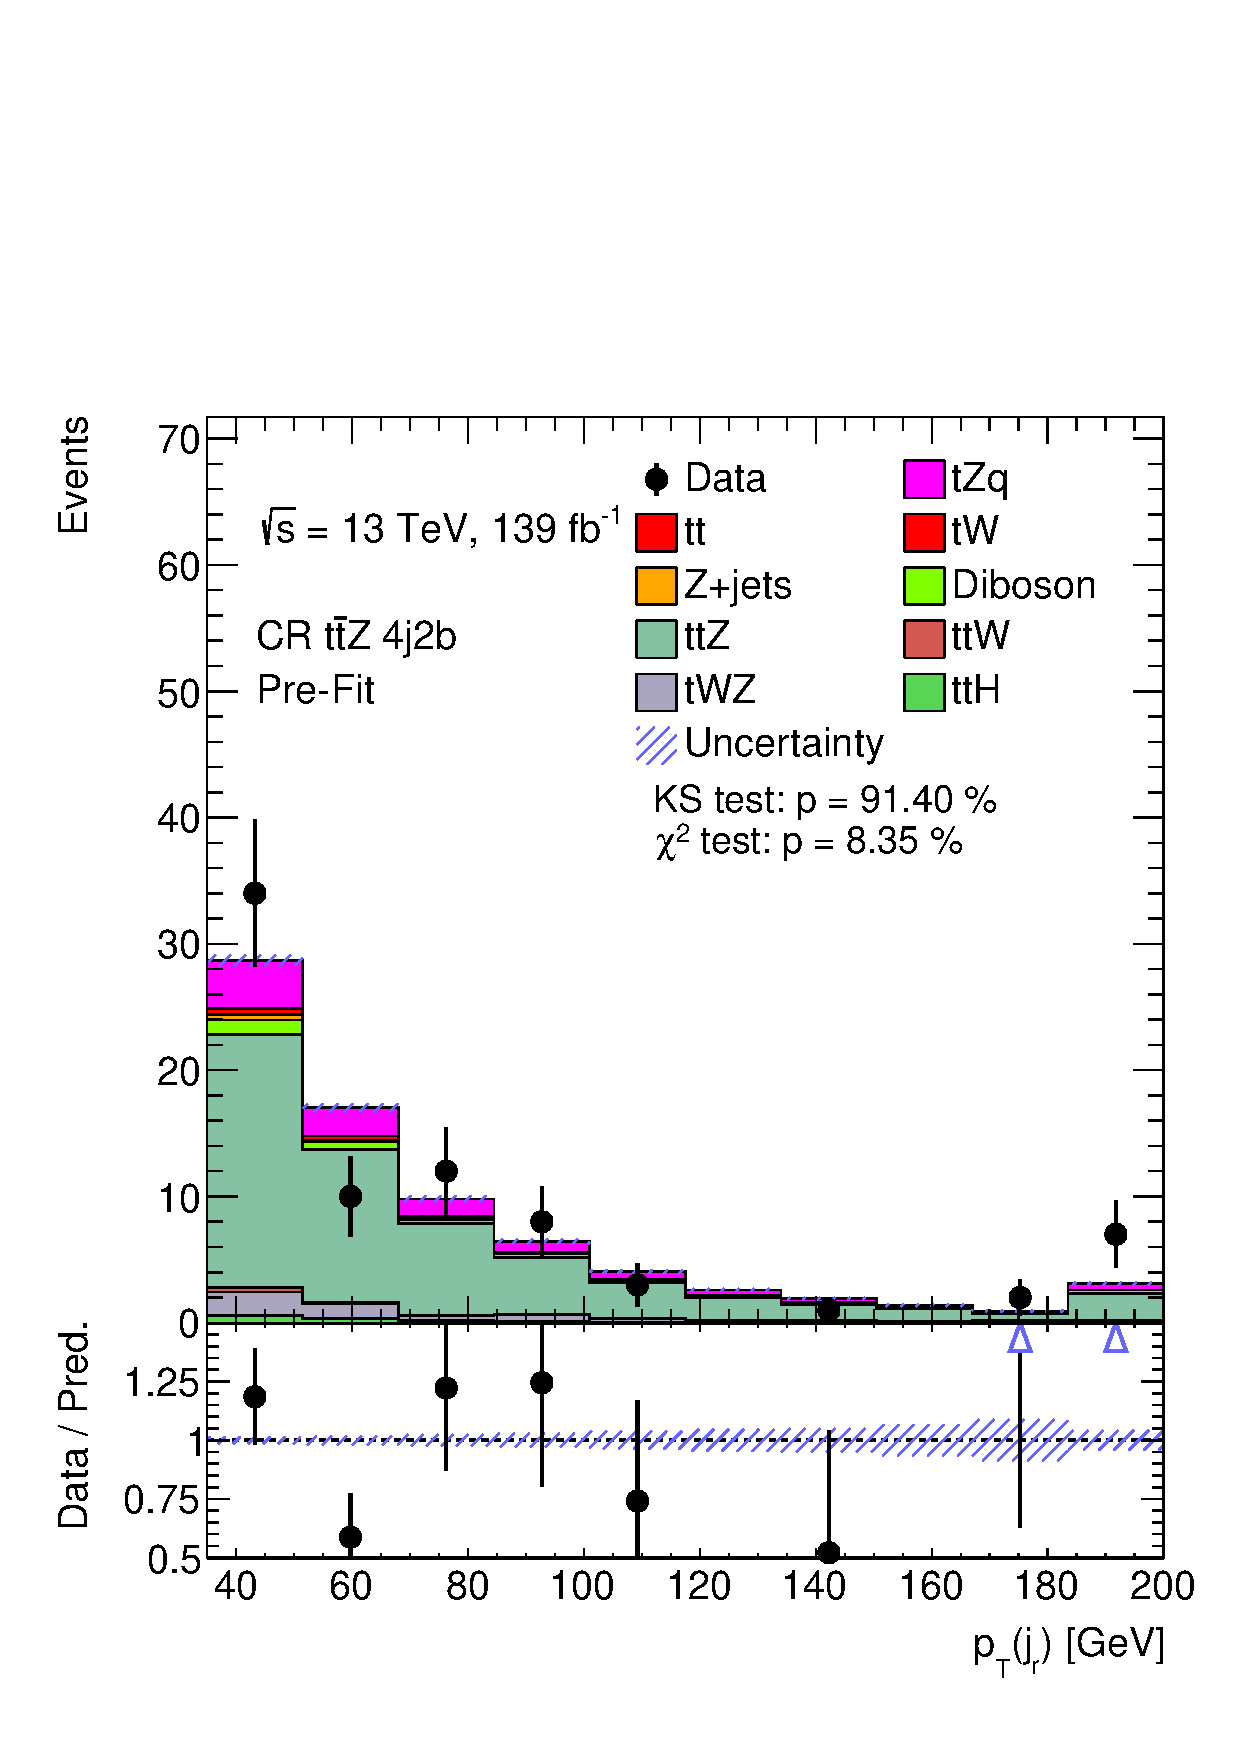
\includegraphics[width=\linewidth]{ubonn-thesis/Chapters/Chapters_06/Figure/Input_distribution/CR_4j2b_ptjf.pdf} 
  \end{subfigure} 
  \newline
  \vspace*{0.4cm}
  \begin{subfigure}[b]{0.33\linewidth}
    \centering
    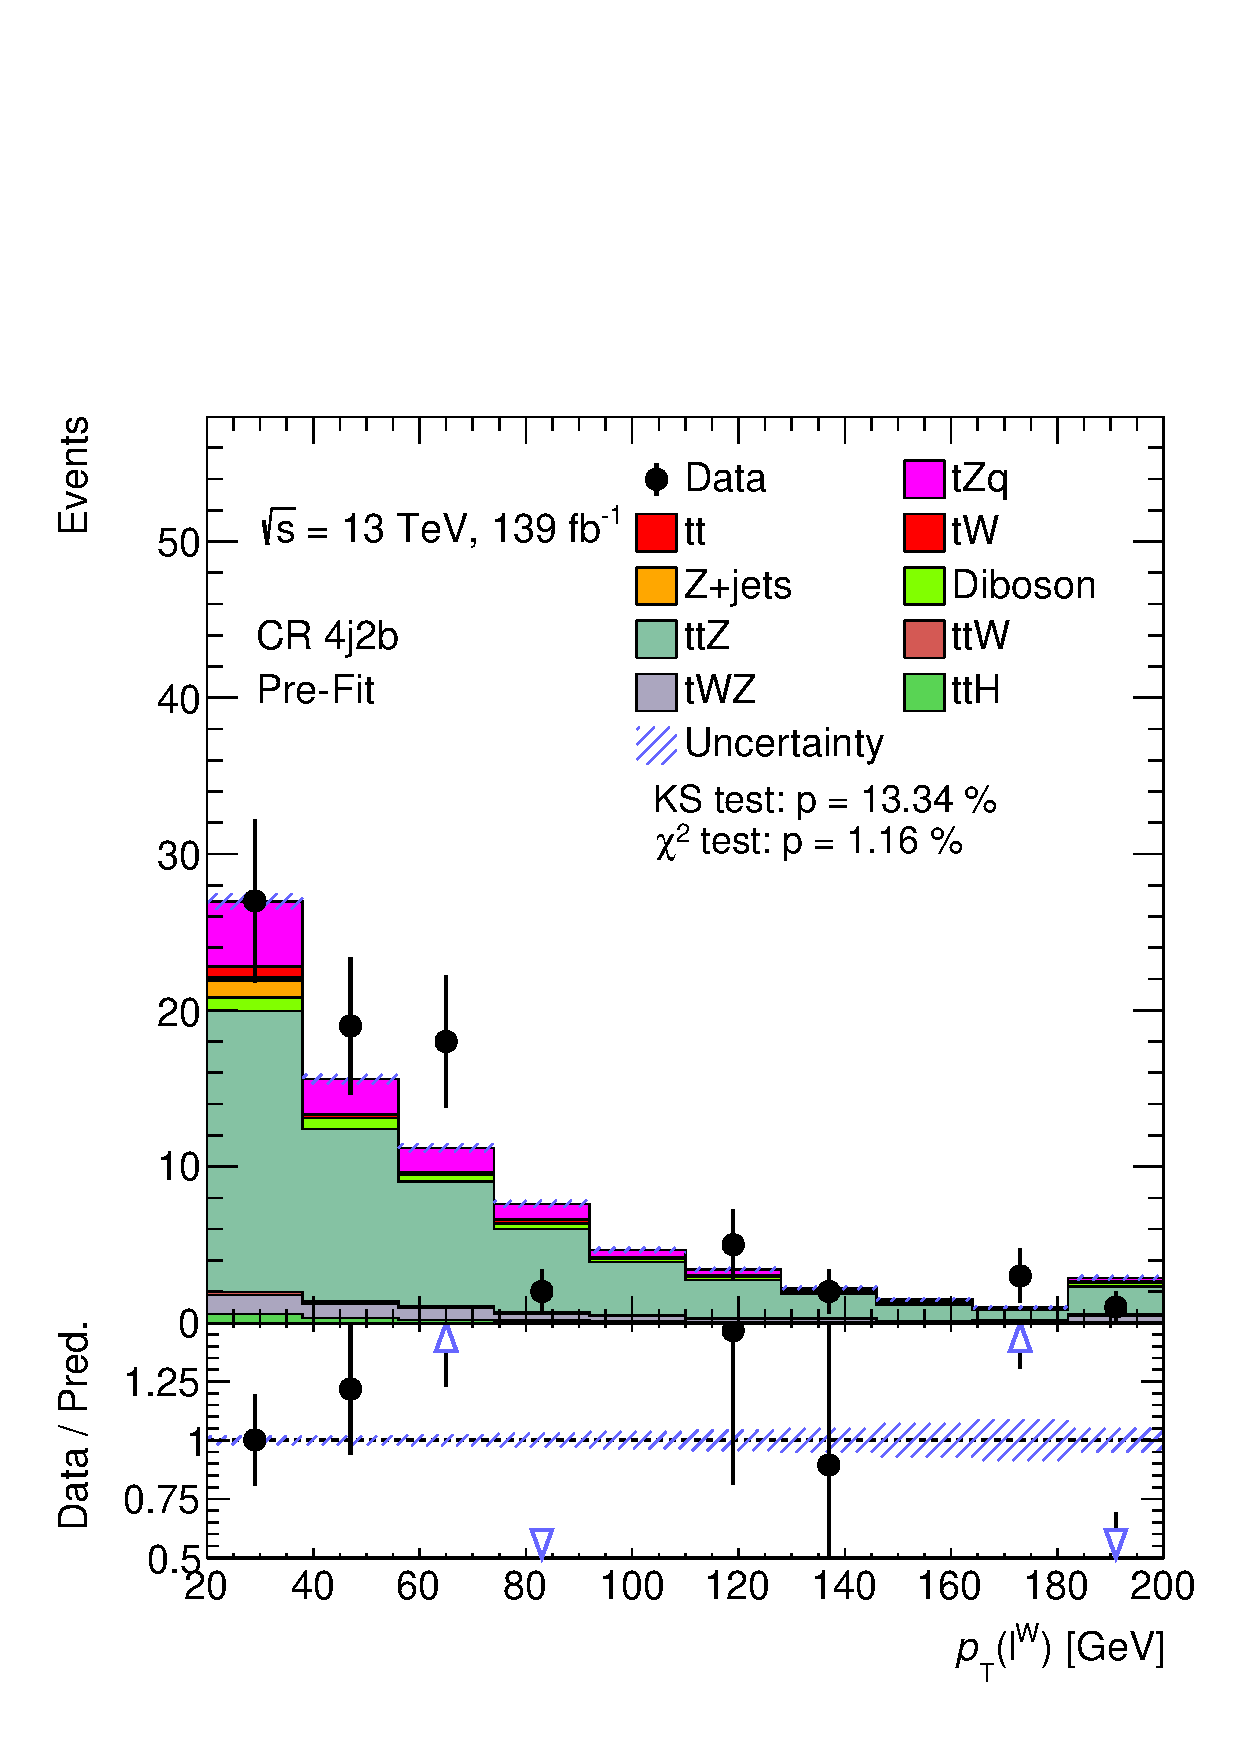
\includegraphics[width=\linewidth]{ubonn-thesis/Chapters/Chapters_06/Figure/Input_distribution/CR_4j2b_lepW_pt.pdf} 
  \end{subfigure}%%
  \begin{subfigure}[b]{0.33\linewidth}
    \centering
    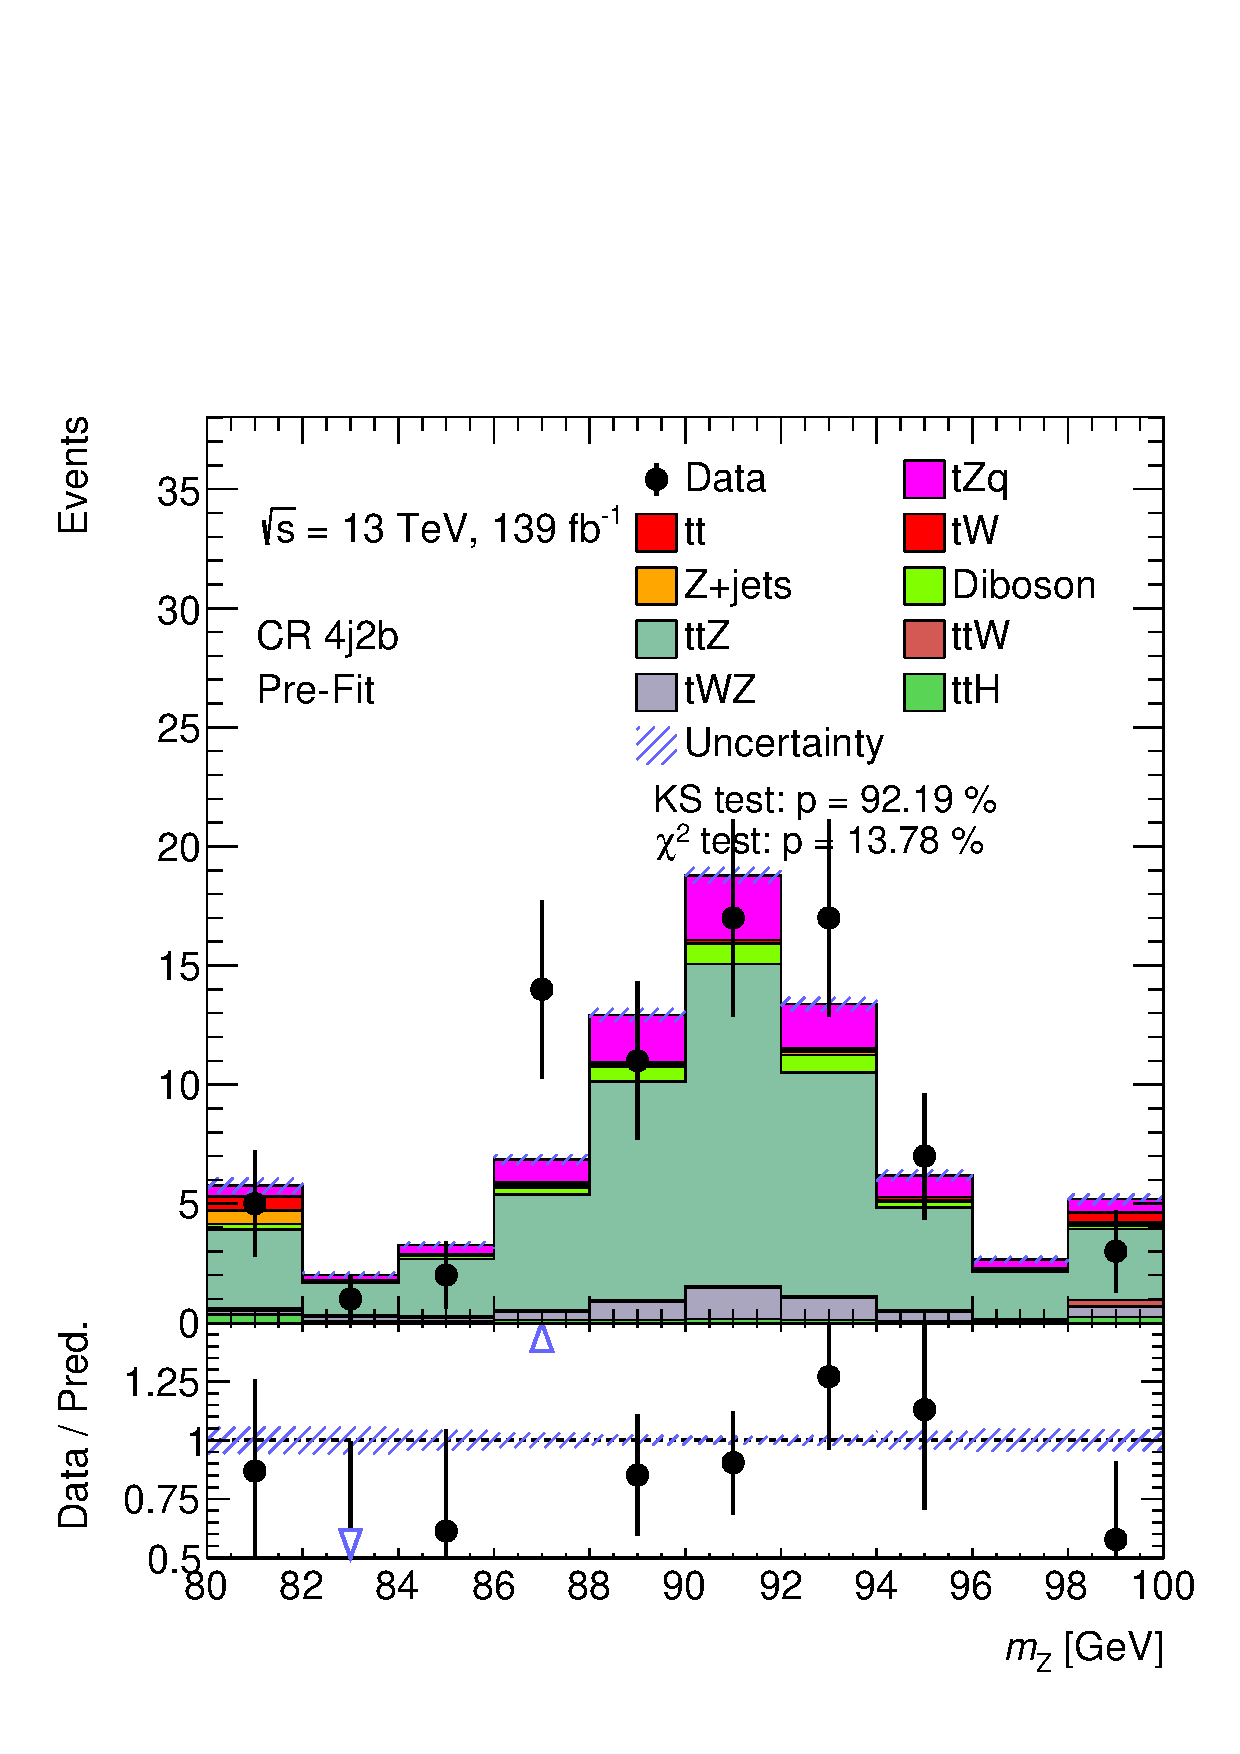
\includegraphics[width=\linewidth]{ubonn-thesis/Chapters/Chapters_06/Figure/Input_distribution/CR_4j2b_MZ.pdf} 
  \end{subfigure}
  \begin{subfigure}[b]{0.33\linewidth}
    \centering
    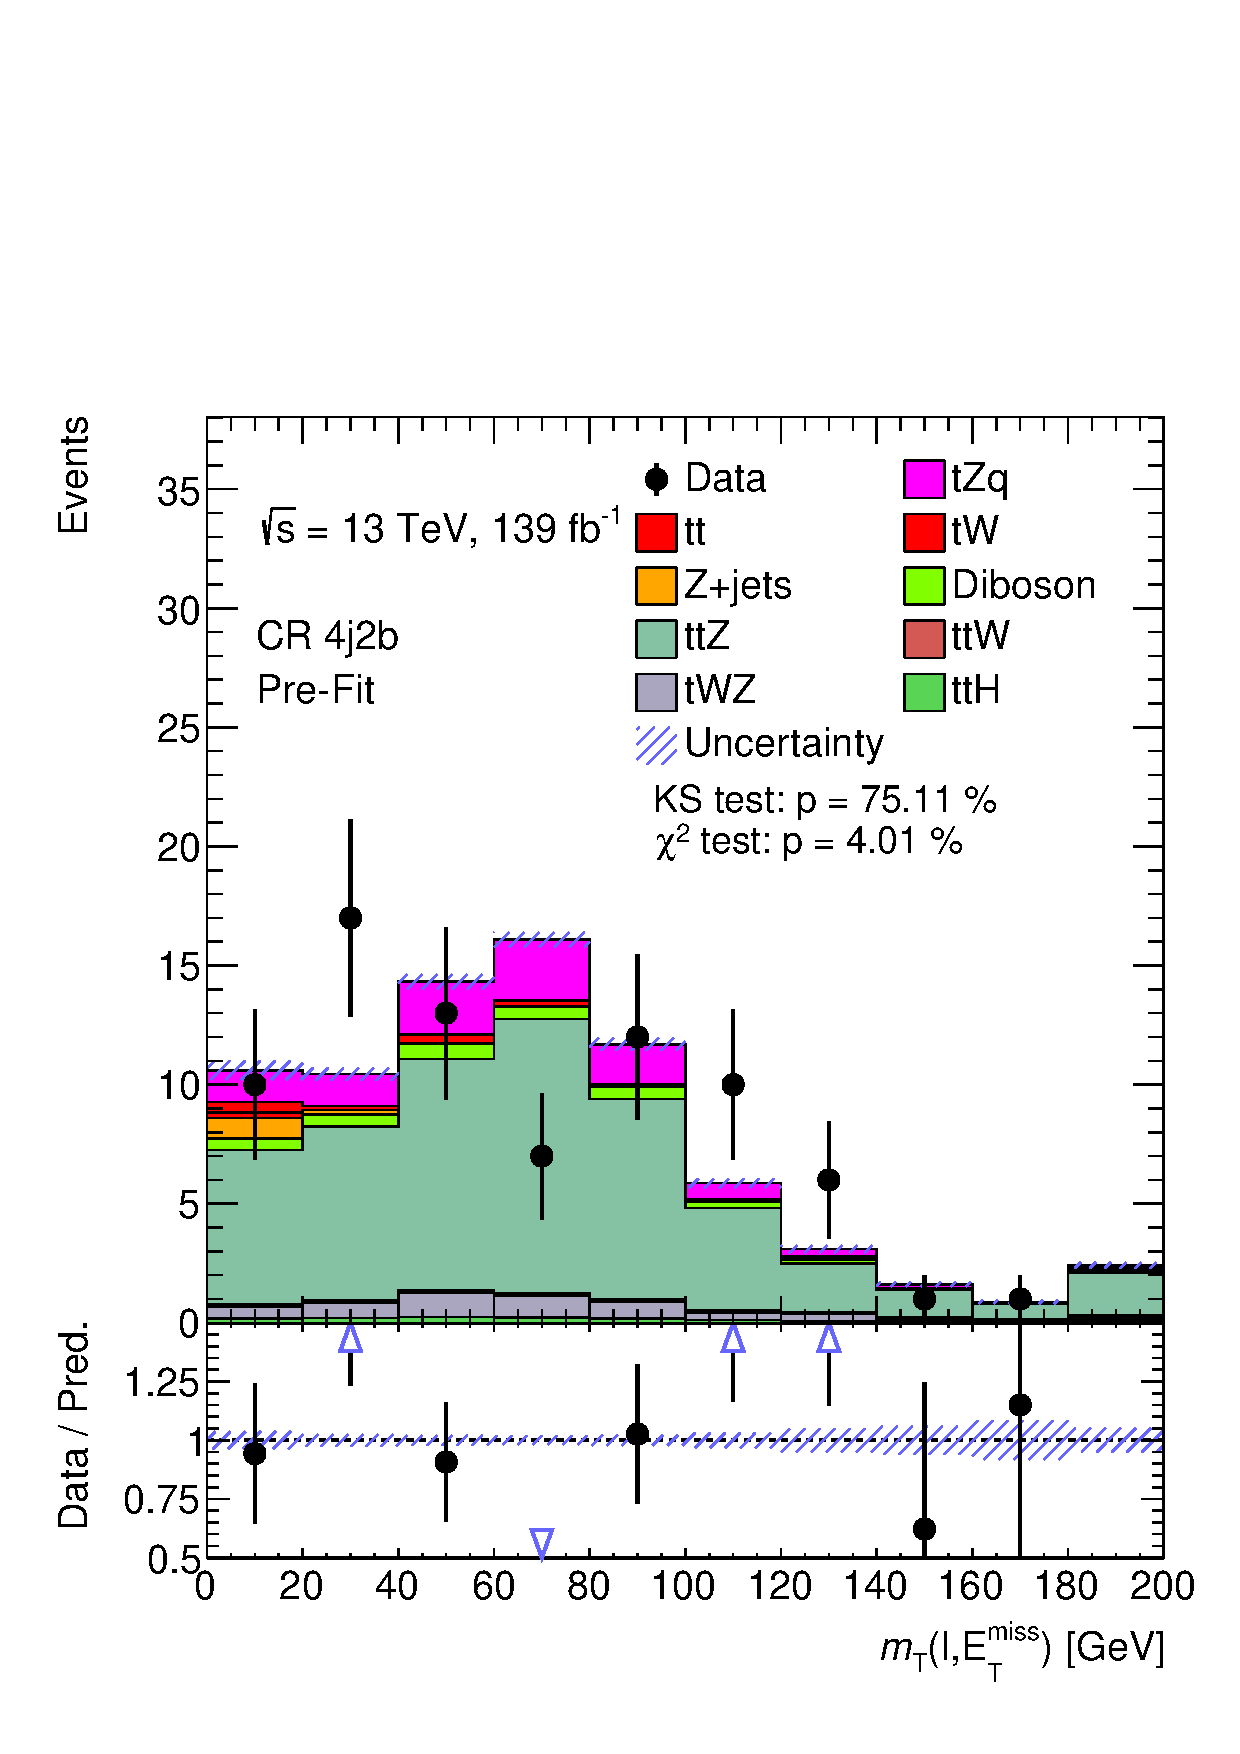
\includegraphics[width=\linewidth]{ubonn-thesis/Chapters/Chapters_06/Figure/Input_distribution/CR_4j2b_mtW.pdf} 
  \end{subfigure} 
  \newline
  \vspace*{0.4cm}
  \begin{subfigure}[b]{0.33\linewidth}
    \centering
    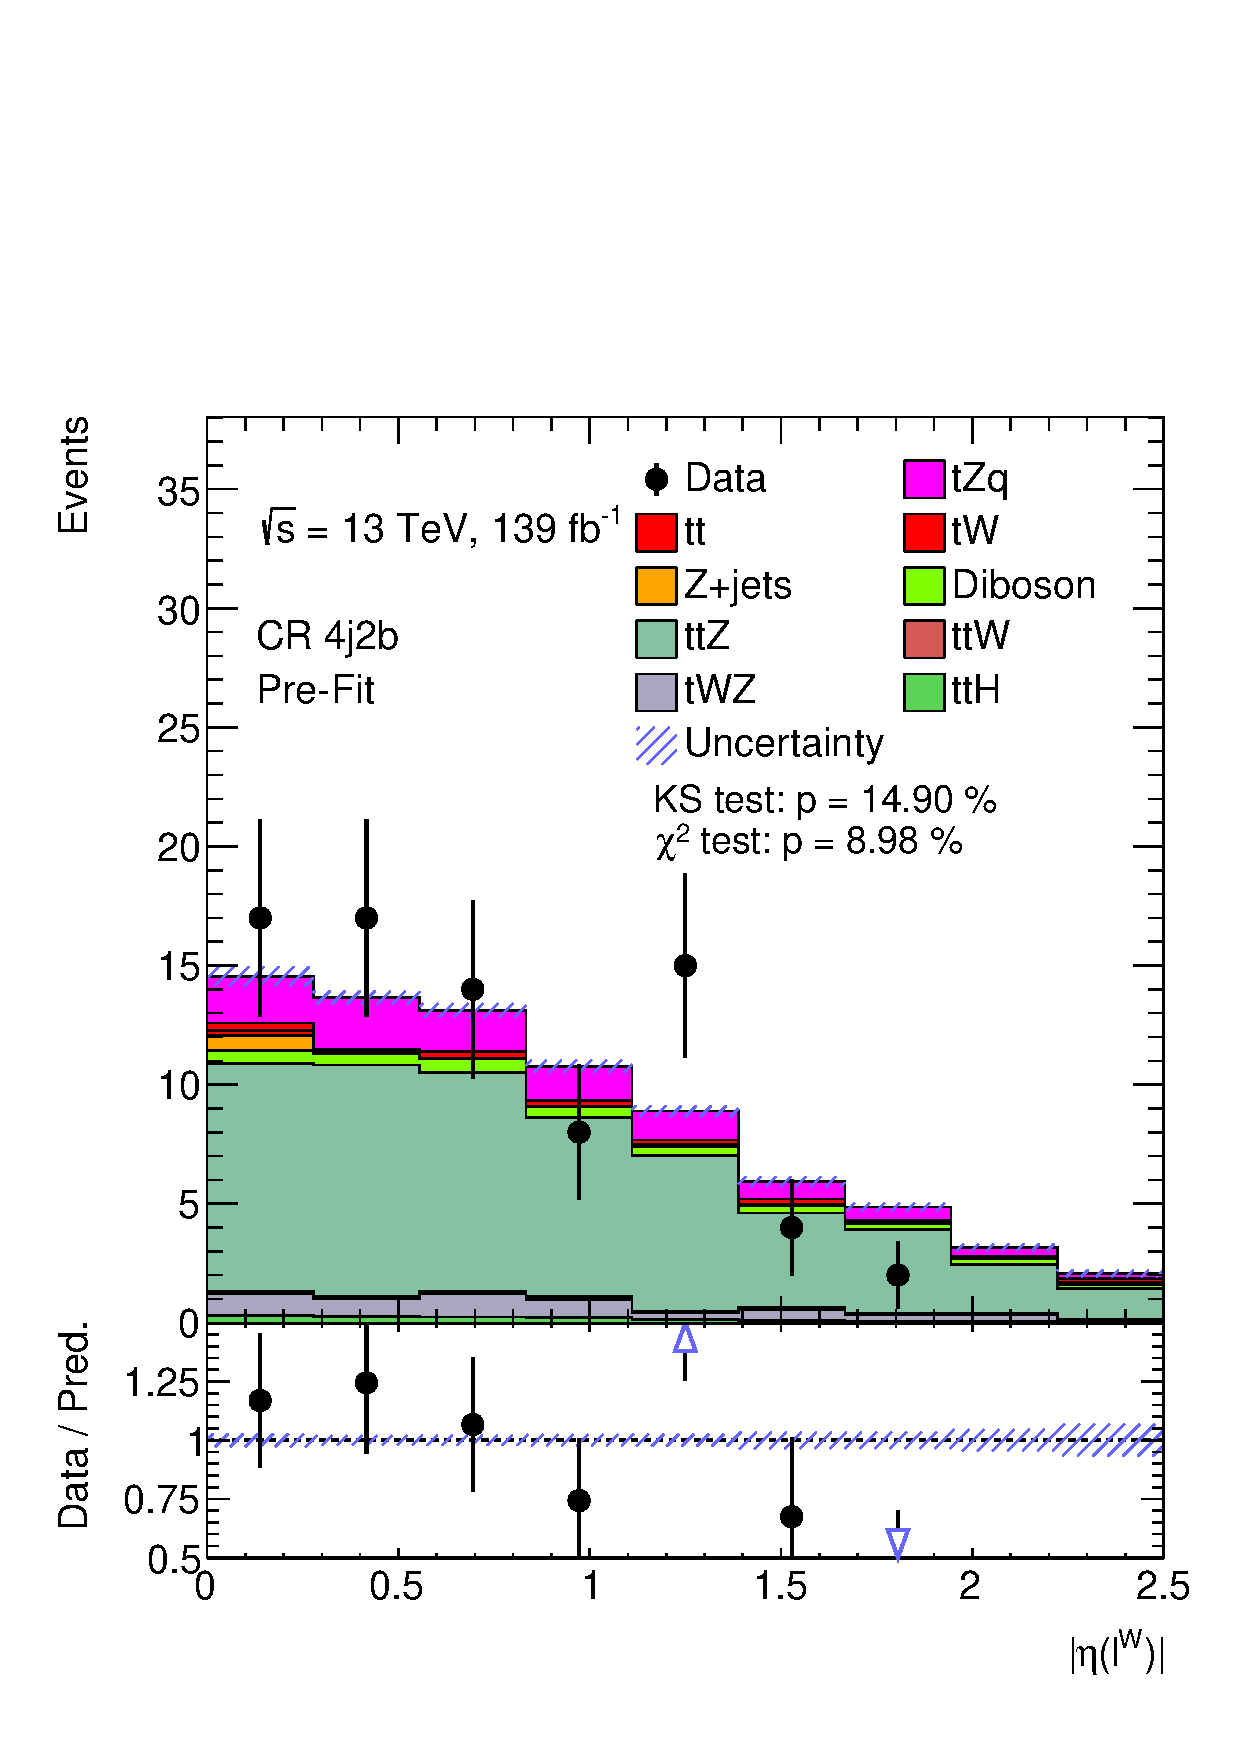
\includegraphics[width=\linewidth]{ubonn-thesis/Chapters/Chapters_06/Figure/Input_distribution/CR_4j2b_lepW_eta.pdf} 
  \end{subfigure}%%
  \begin{subfigure}[b]{0.33\linewidth}
    \centering
    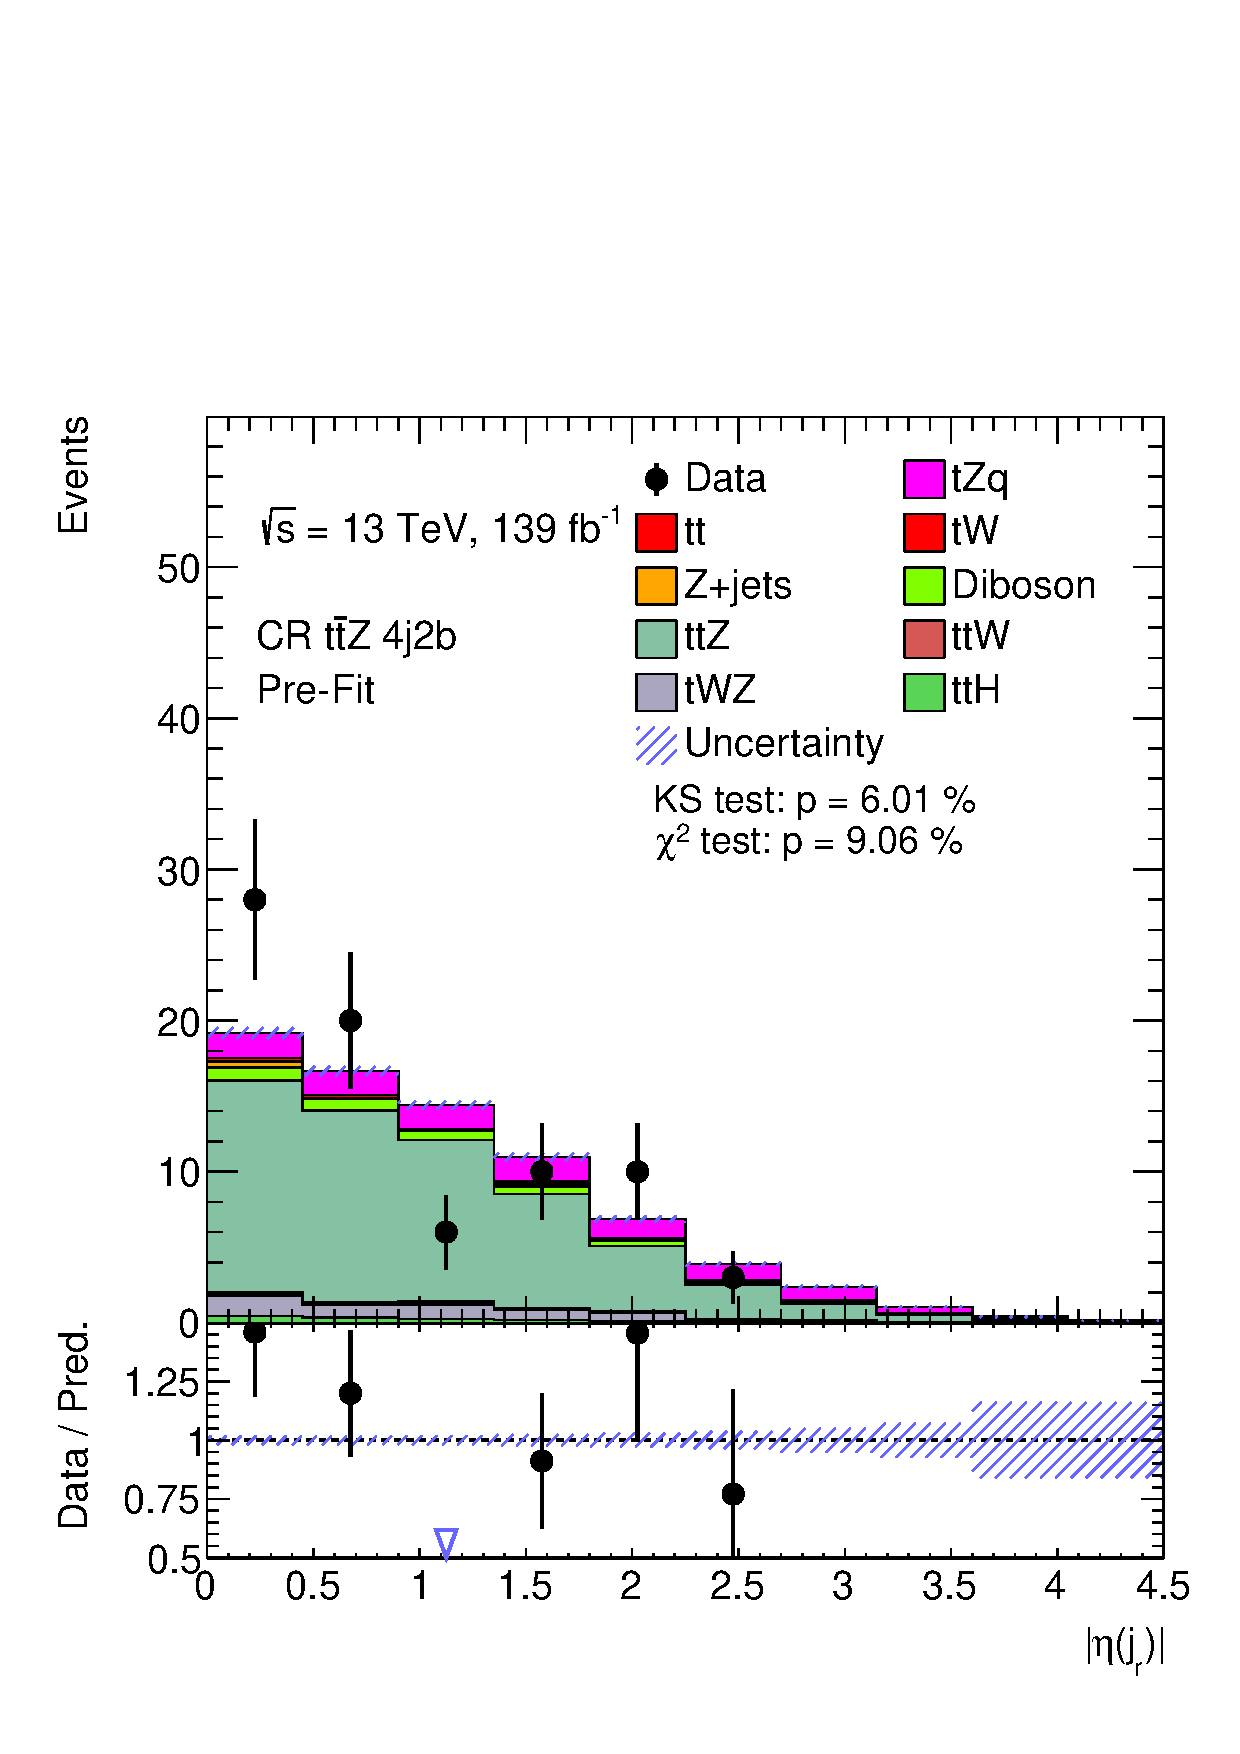
\includegraphics[width=\linewidth]{ubonn-thesis/Chapters/Chapters_06/Figure/Input_distribution/CR_4j2b_etajf.pdf} 
  \end{subfigure}
  \begin{subfigure}[b]{0.33\linewidth}
    \centering
    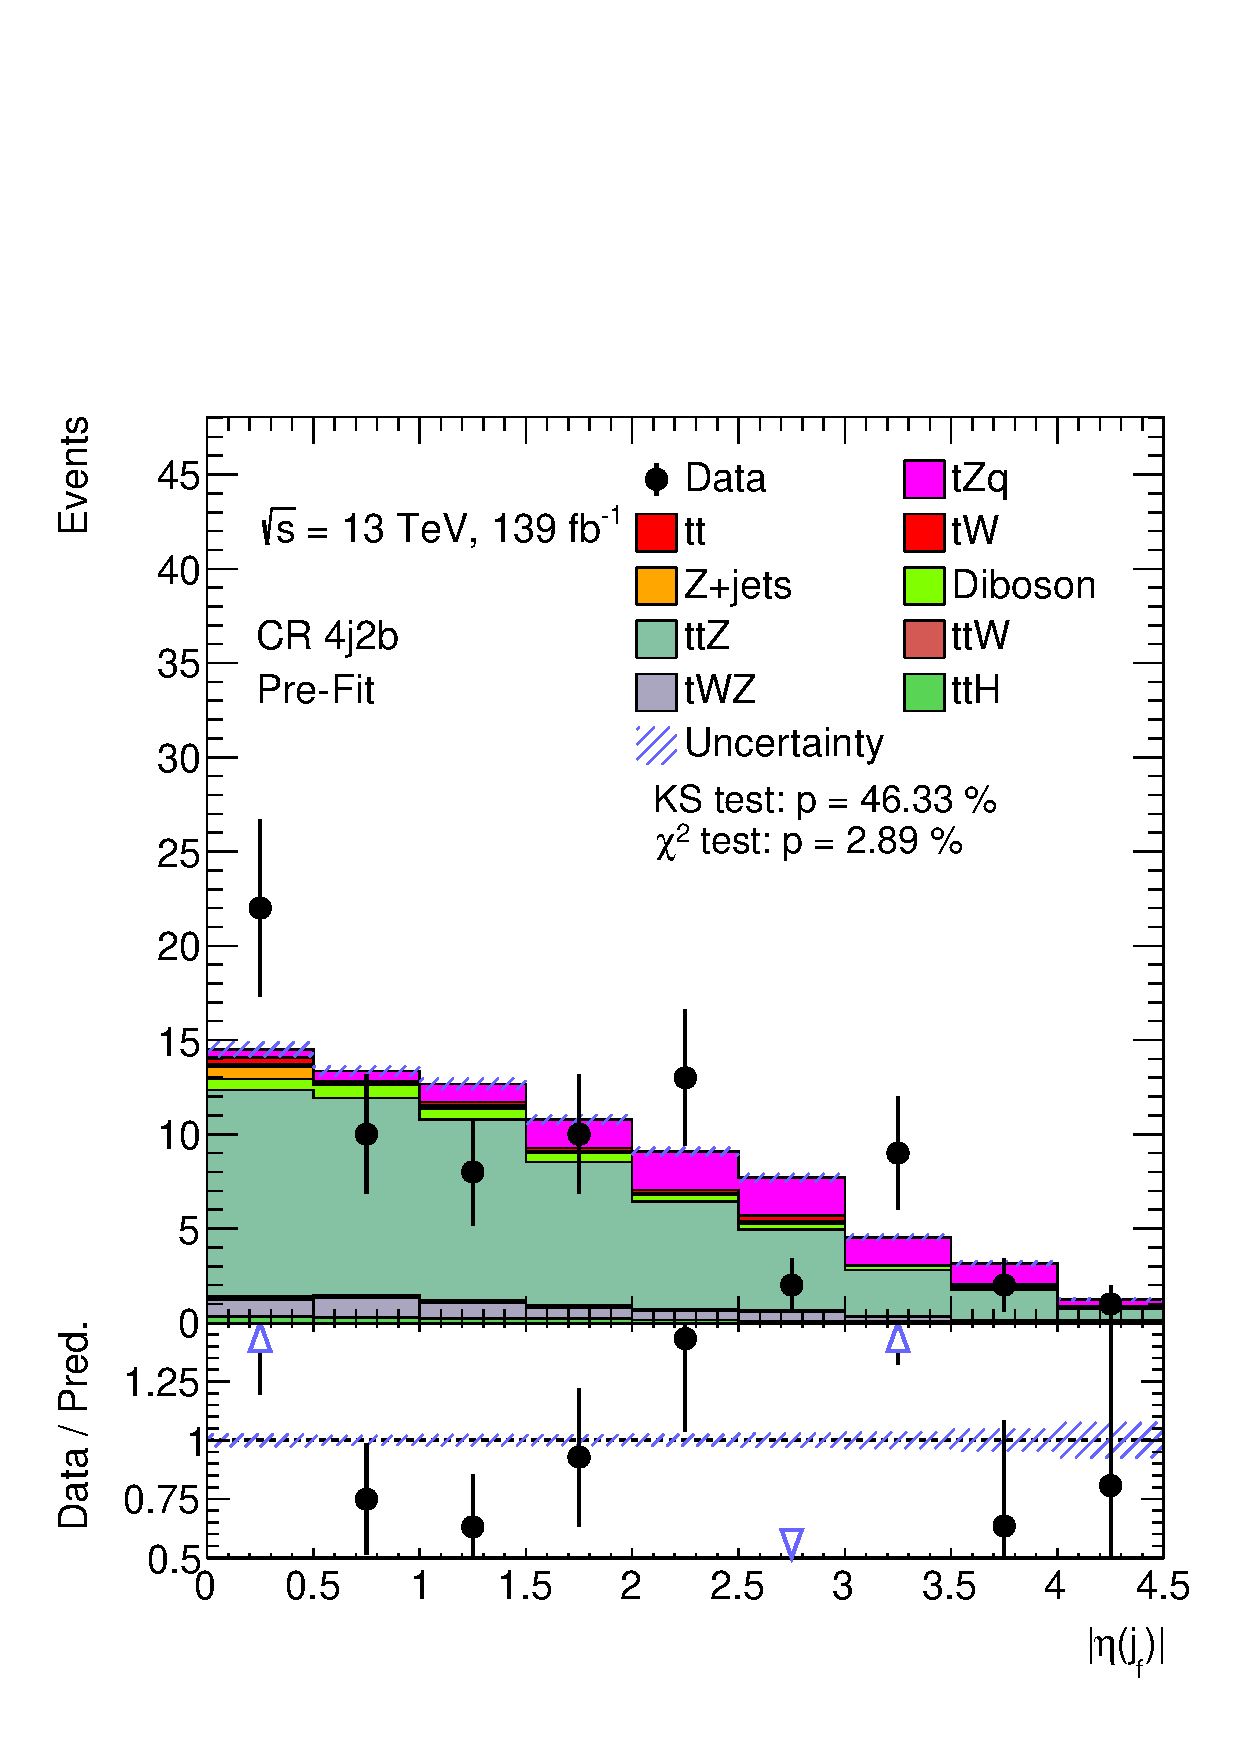
\includegraphics[width=\linewidth]{ubonn-thesis/Chapters/Chapters_06/Figure/Input_distribution/CR_4j2b_forwardjet_eta.pdf} 
  \end{subfigure} 
   \caption{Stacked kinematic plots of neural-network training variables of the CR 4j2b, in order of significance. Both signal and backgrounds are normalised to the expected number of events before the fit. The uncertainty band includes statistical uncertainties for signal and backgrounds}
  \label{fig_control4} 
\end{figure}


\begin{figure}[!h] 
  \begin{subfigure}[b]{0.33\linewidth}
    \centering
    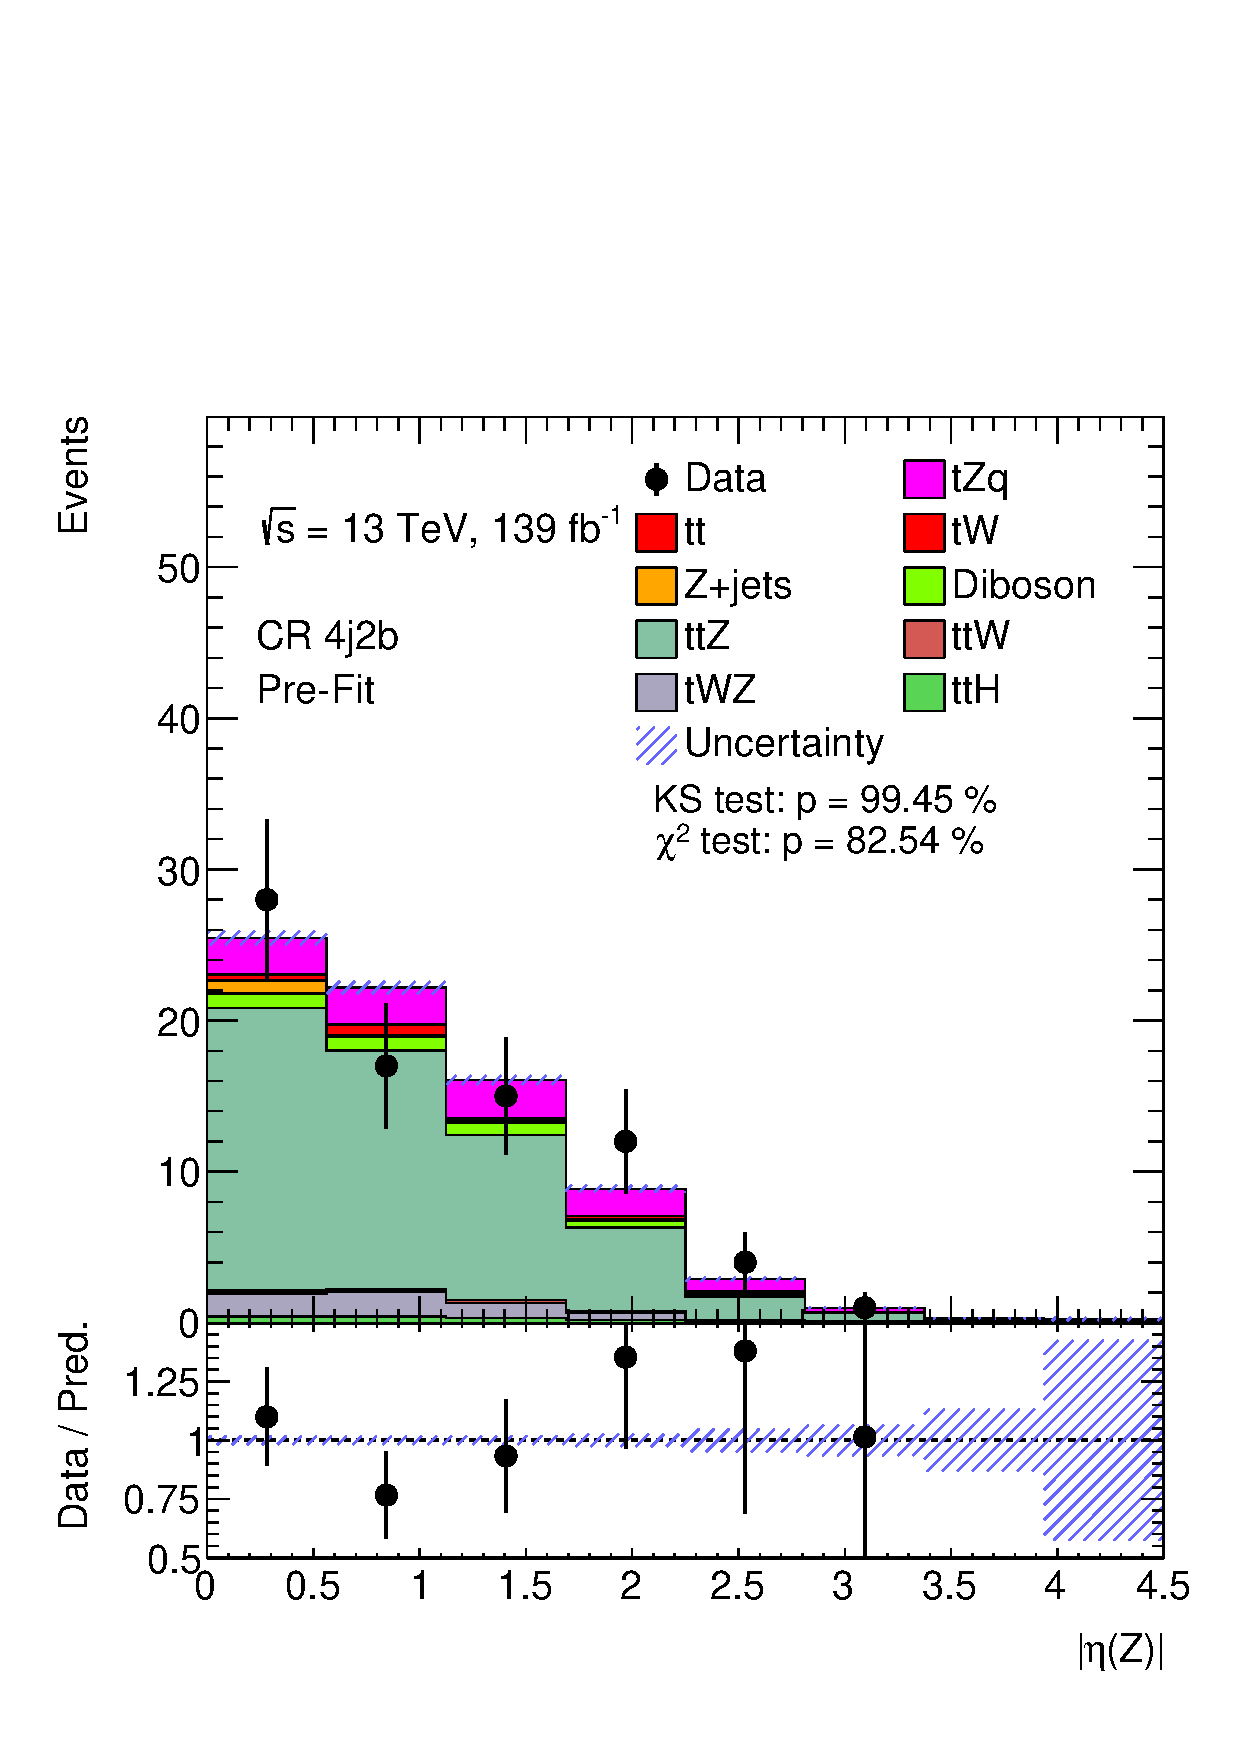
\includegraphics[width=\linewidth]{ubonn-thesis/Chapters/Chapters_06/Figure/Input_distribution/CR_4j2b_Z_eta.pdf} 
  \end{subfigure} 
  \begin{subfigure}[b]{0.33\linewidth}
    \centering
    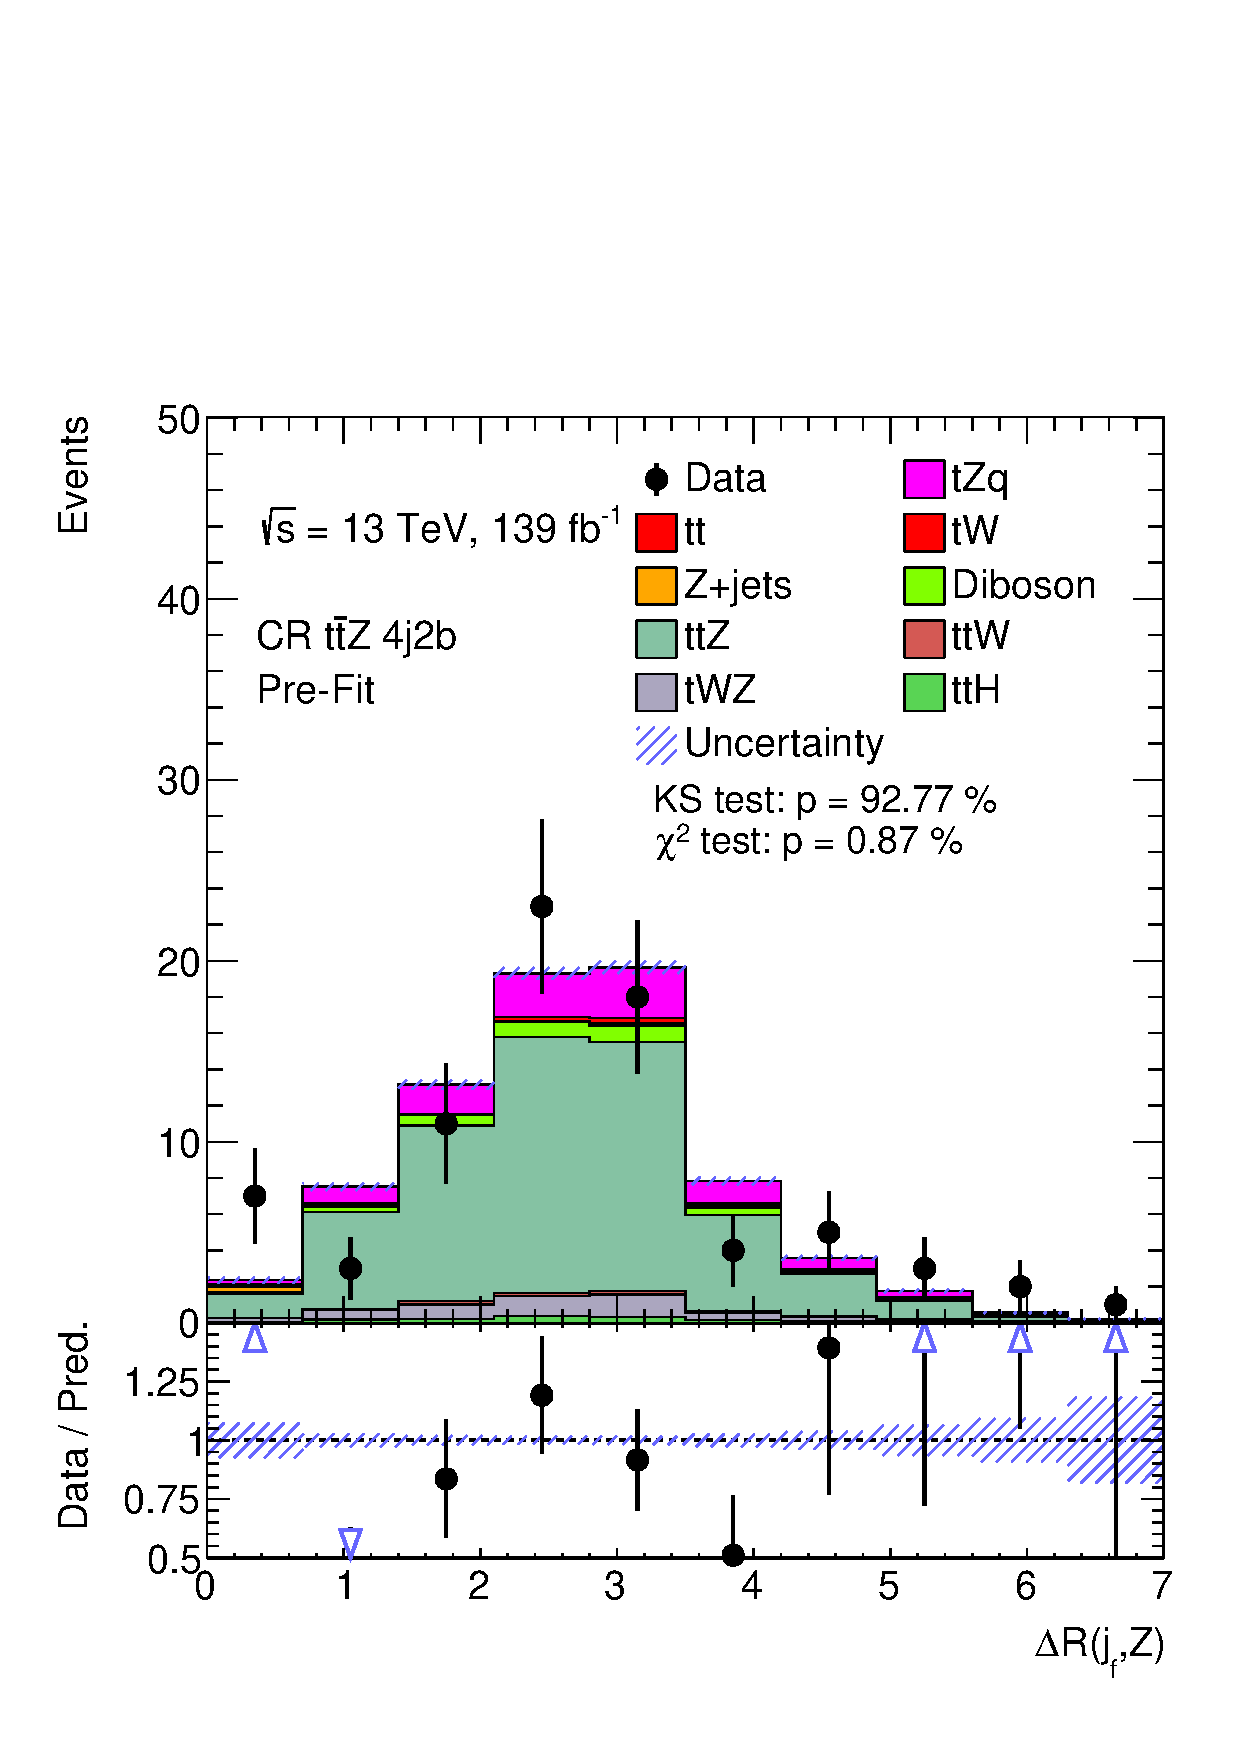
\includegraphics[width=\linewidth]{ubonn-thesis/Chapters/Chapters_06/Figure/Input_distribution/CR_4j2b_dRjfZ.pdf} 
  \end{subfigure}%% 
  \begin{subfigure}[b]{0.33\linewidth}
    \centering
    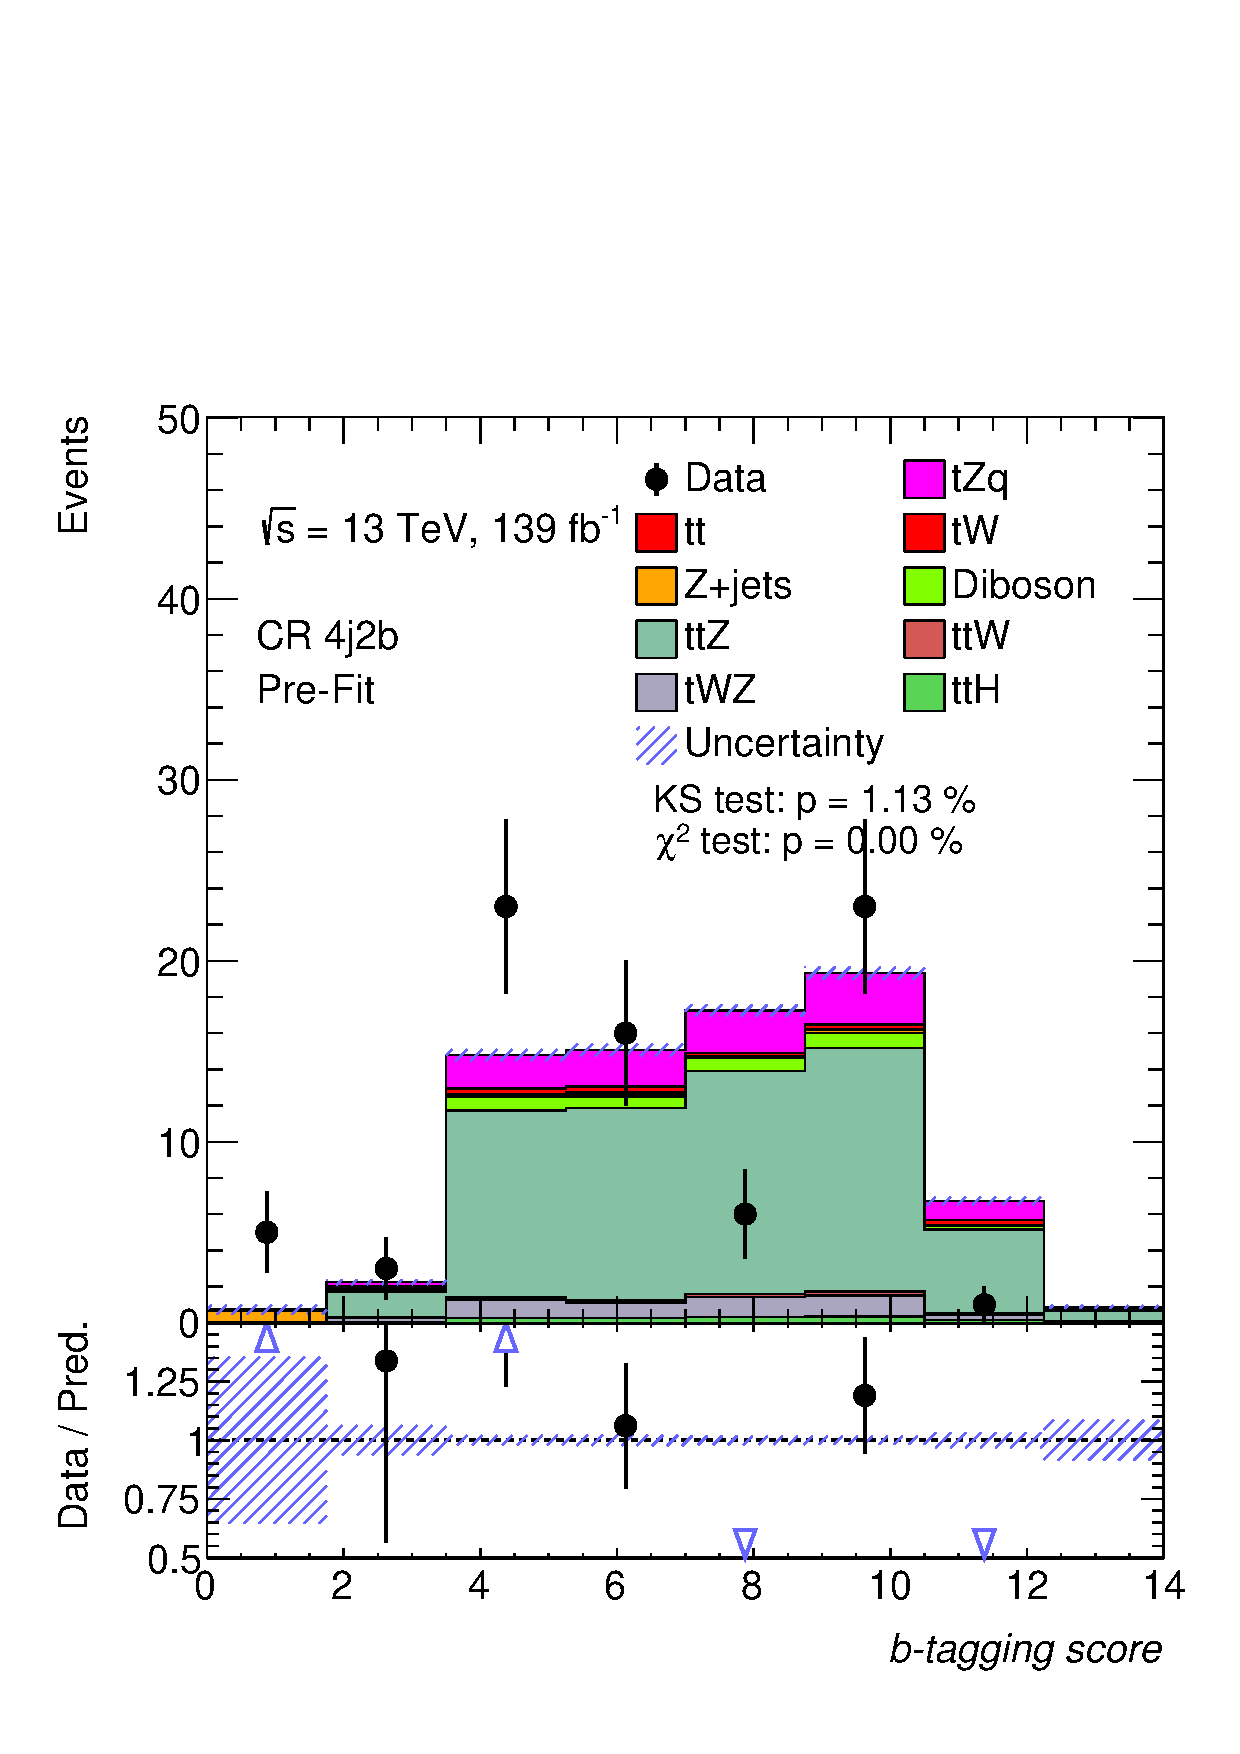
\includegraphics[width=\linewidth]{ubonn-thesis/Chapters/Chapters_06/Figure/Input_distribution/CR_4j2b_btag.pdf} 
  \end{subfigure}
  \centering
  \begin{subfigure}[b]{0.33\linewidth}
    \centering
    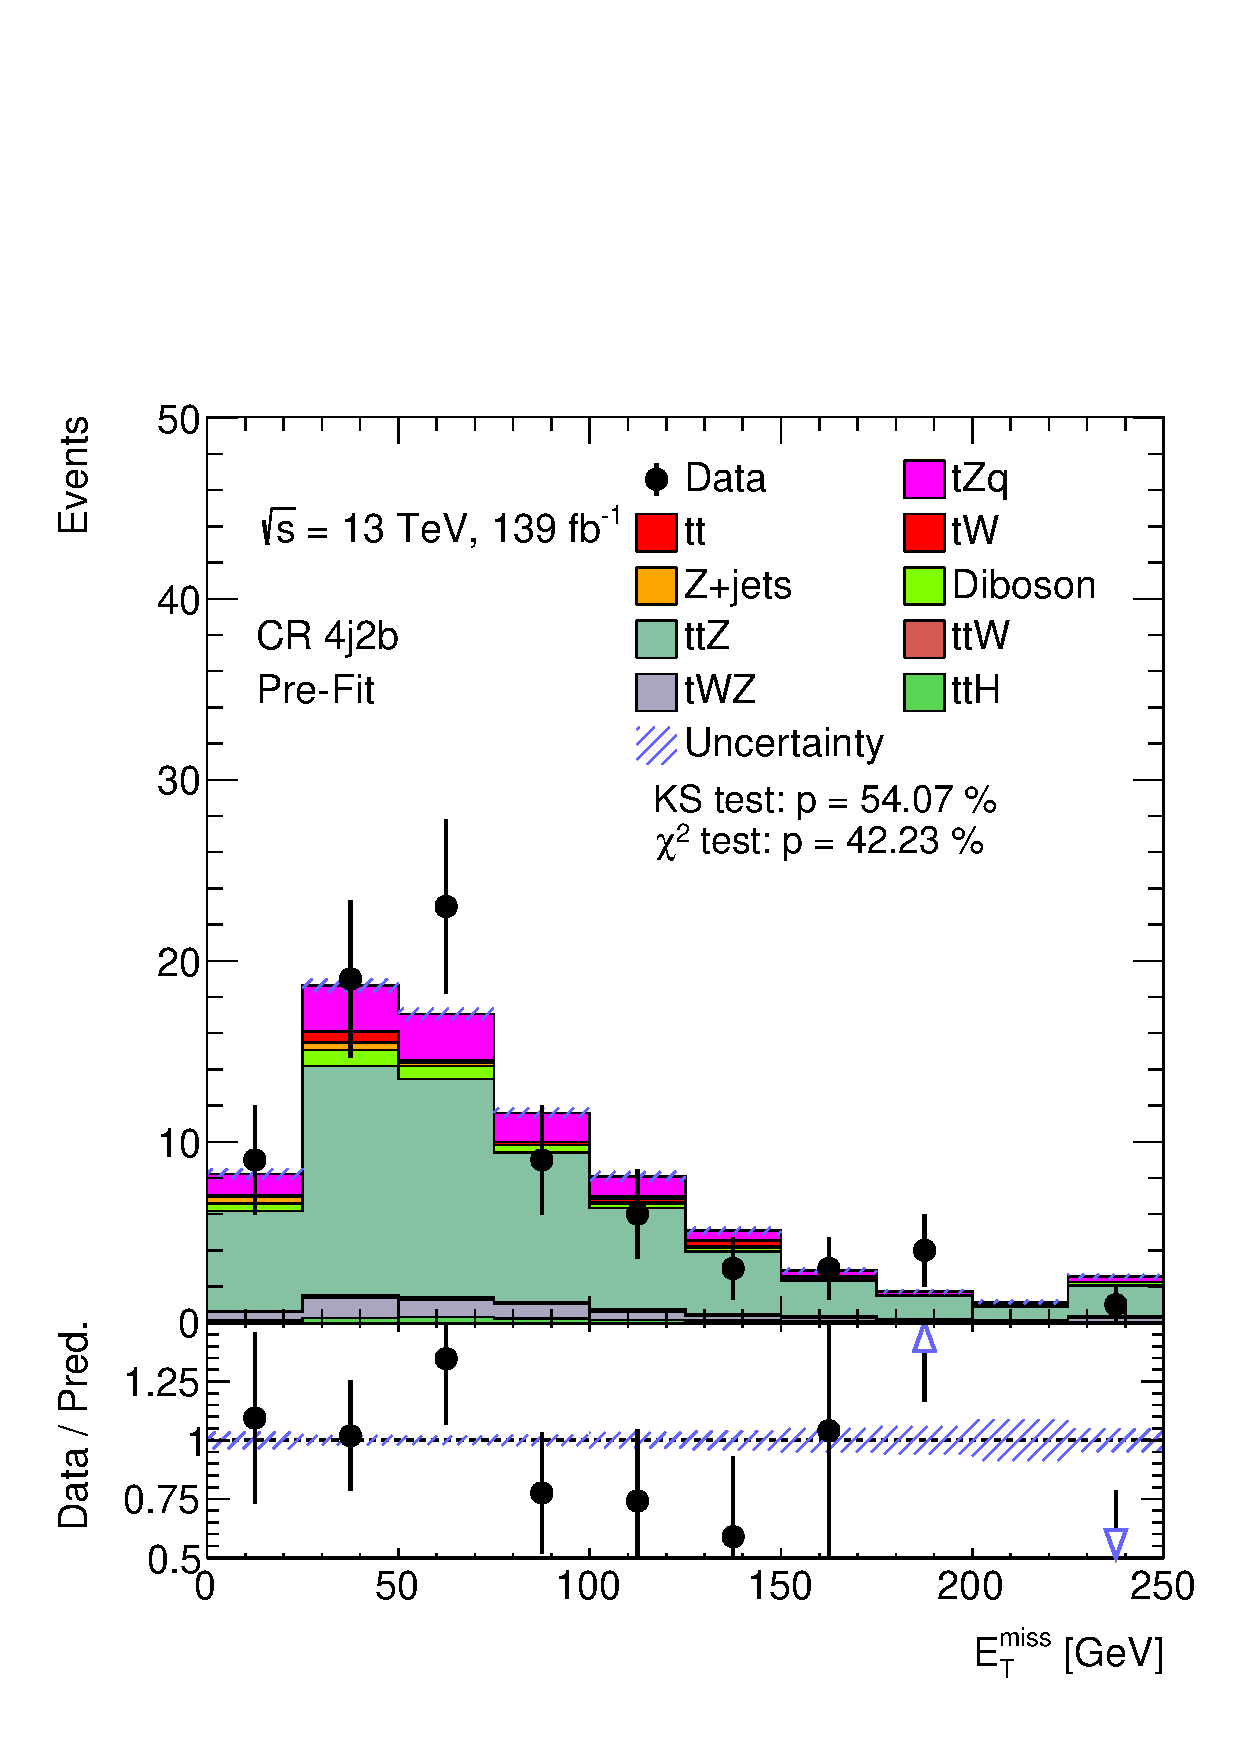
\includegraphics[width=\linewidth]{ubonn-thesis/Chapters/Chapters_06/Figure/Input_distribution/CR_4j2b_MissEt.pdf} 
  \end{subfigure}
  \caption{Stacked kinematic plots of neural-network training variables of the CR 4j2b, in order of significance. Both signal and backgrounds are normalised to the expected number of events before the fit. The uncertainty band includes statistical uncertainties for signal and backgrounds}
  \label{fig_control5}
  \end{figure}

%% clearpage important to put empty space 
\clearpage


\begin{figure}[!h] 
  \begin{subfigure}[b]{0.33\linewidth}
    \centering
    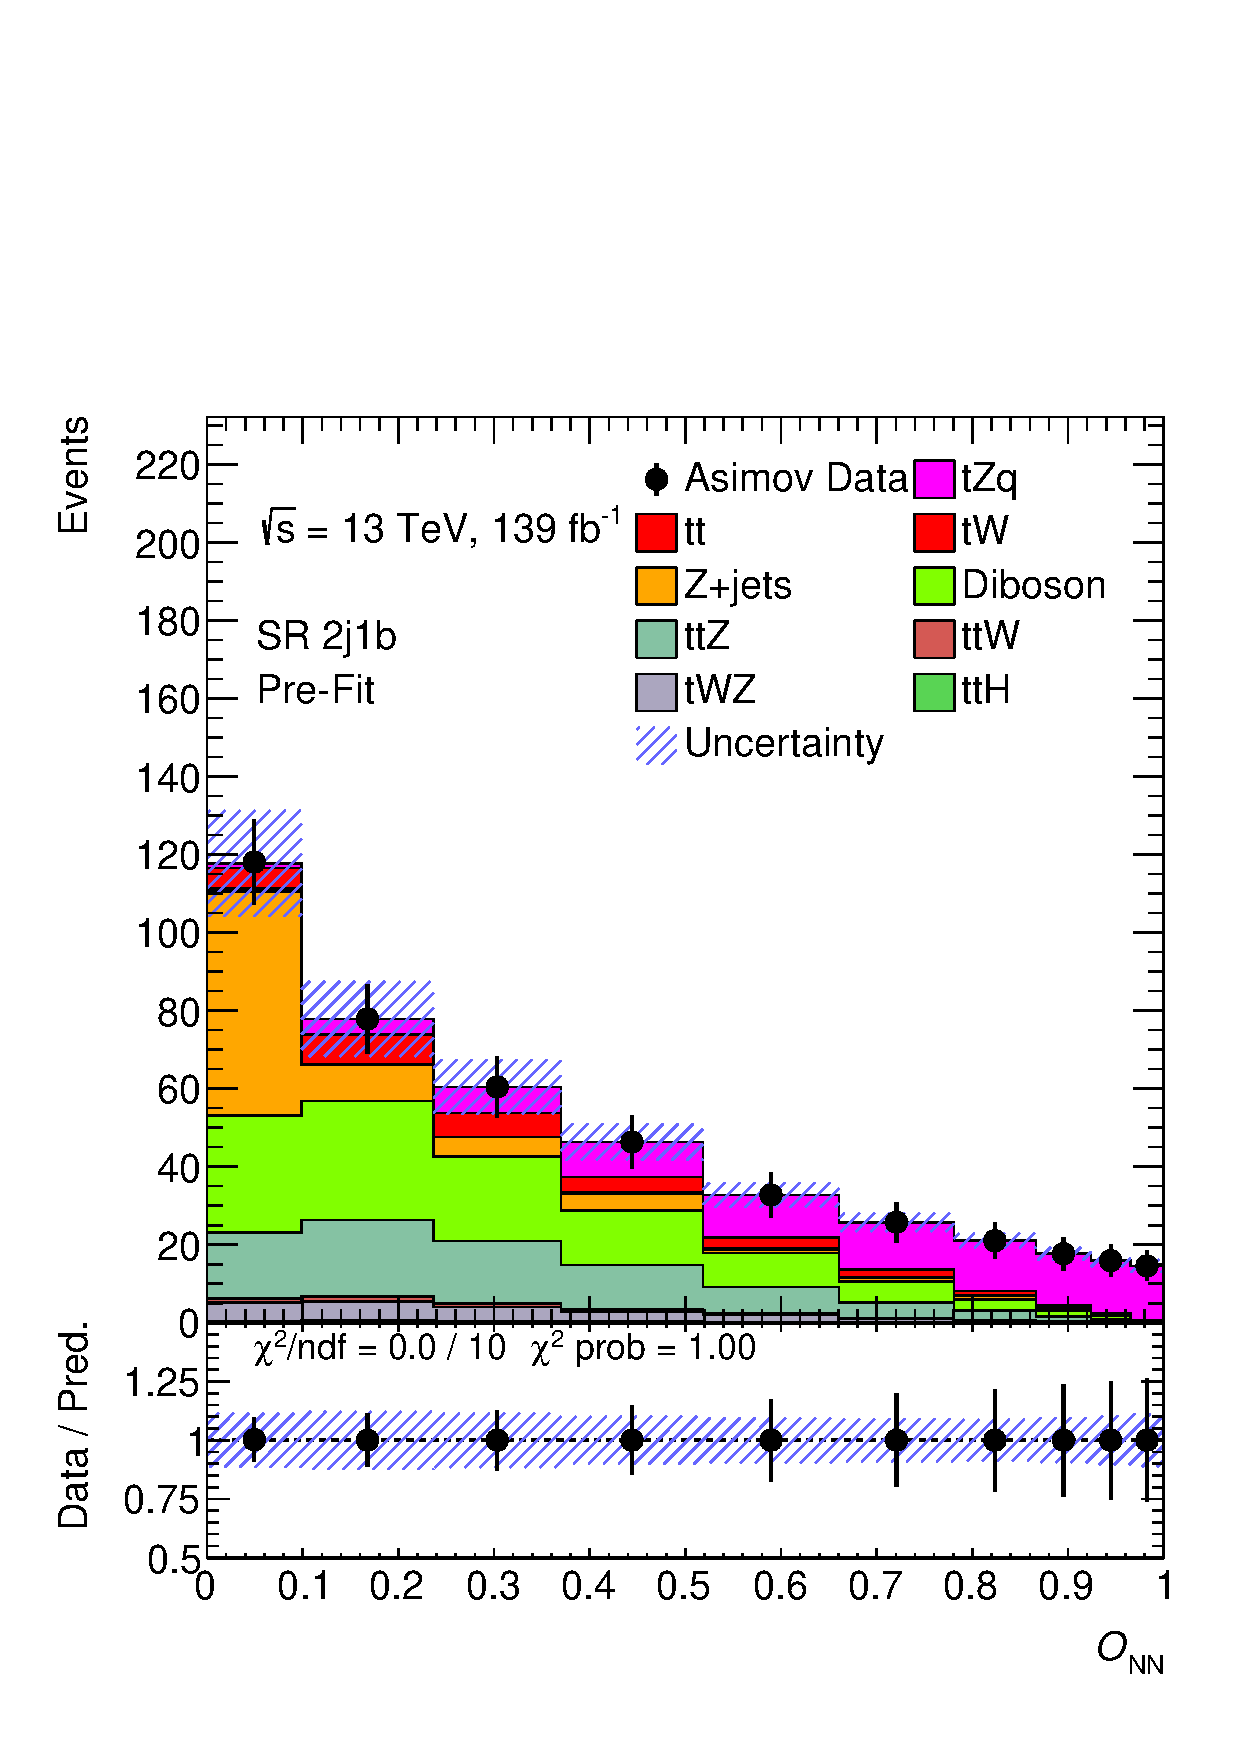
\includegraphics[width=\textwidth]{ubonn-thesis/Chapters/Chapters_07/Figure/Asmiov/SR_2j1b.pdf} 
  \end{subfigure}%% 
  \begin{subfigure}[b]{0.33\linewidth}
    \centering
    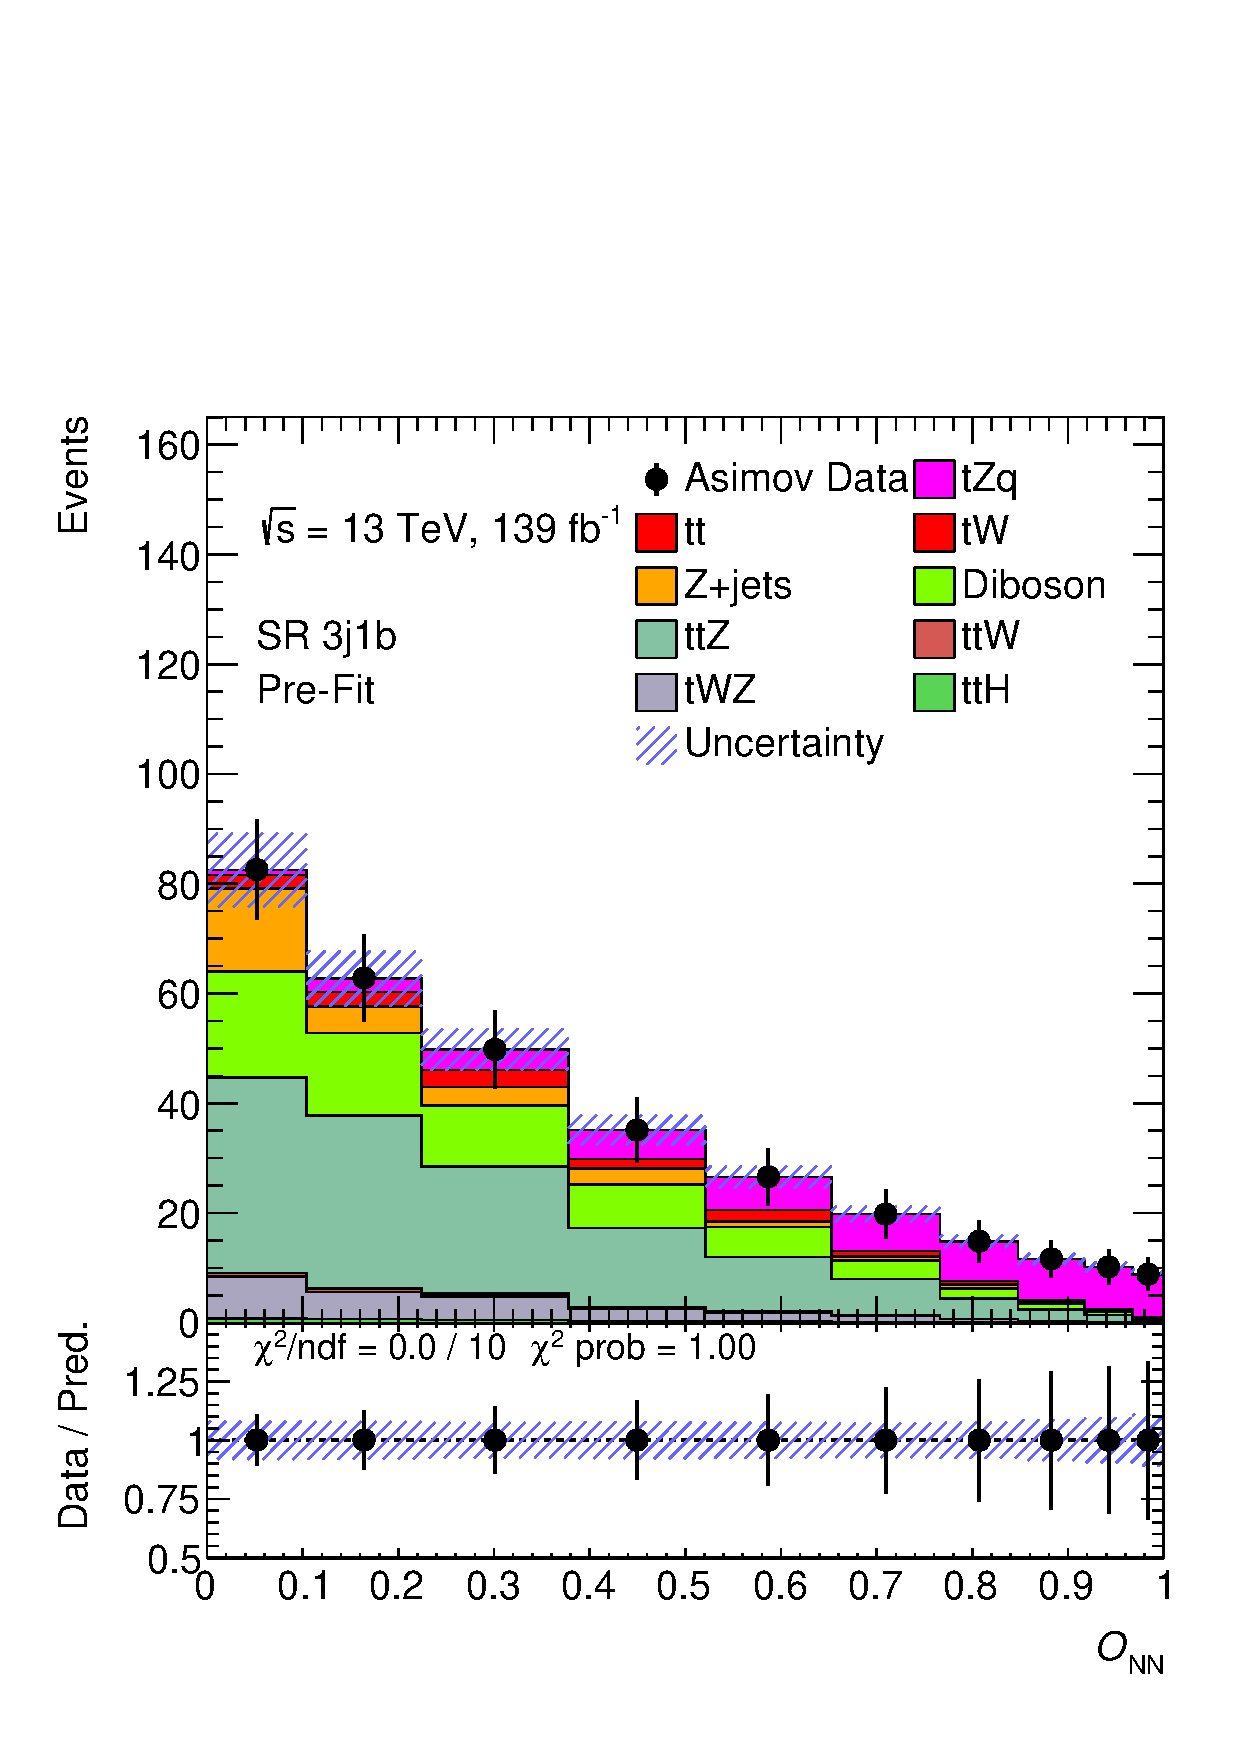
\includegraphics[width=\textwidth]{ubonn-thesis/Chapters/Chapters_07/Figure/Asmiov/SR_3j1b.pdf} 
  \end{subfigure} 
  \begin{subfigure}[b]{0.33\linewidth}
    \centering
    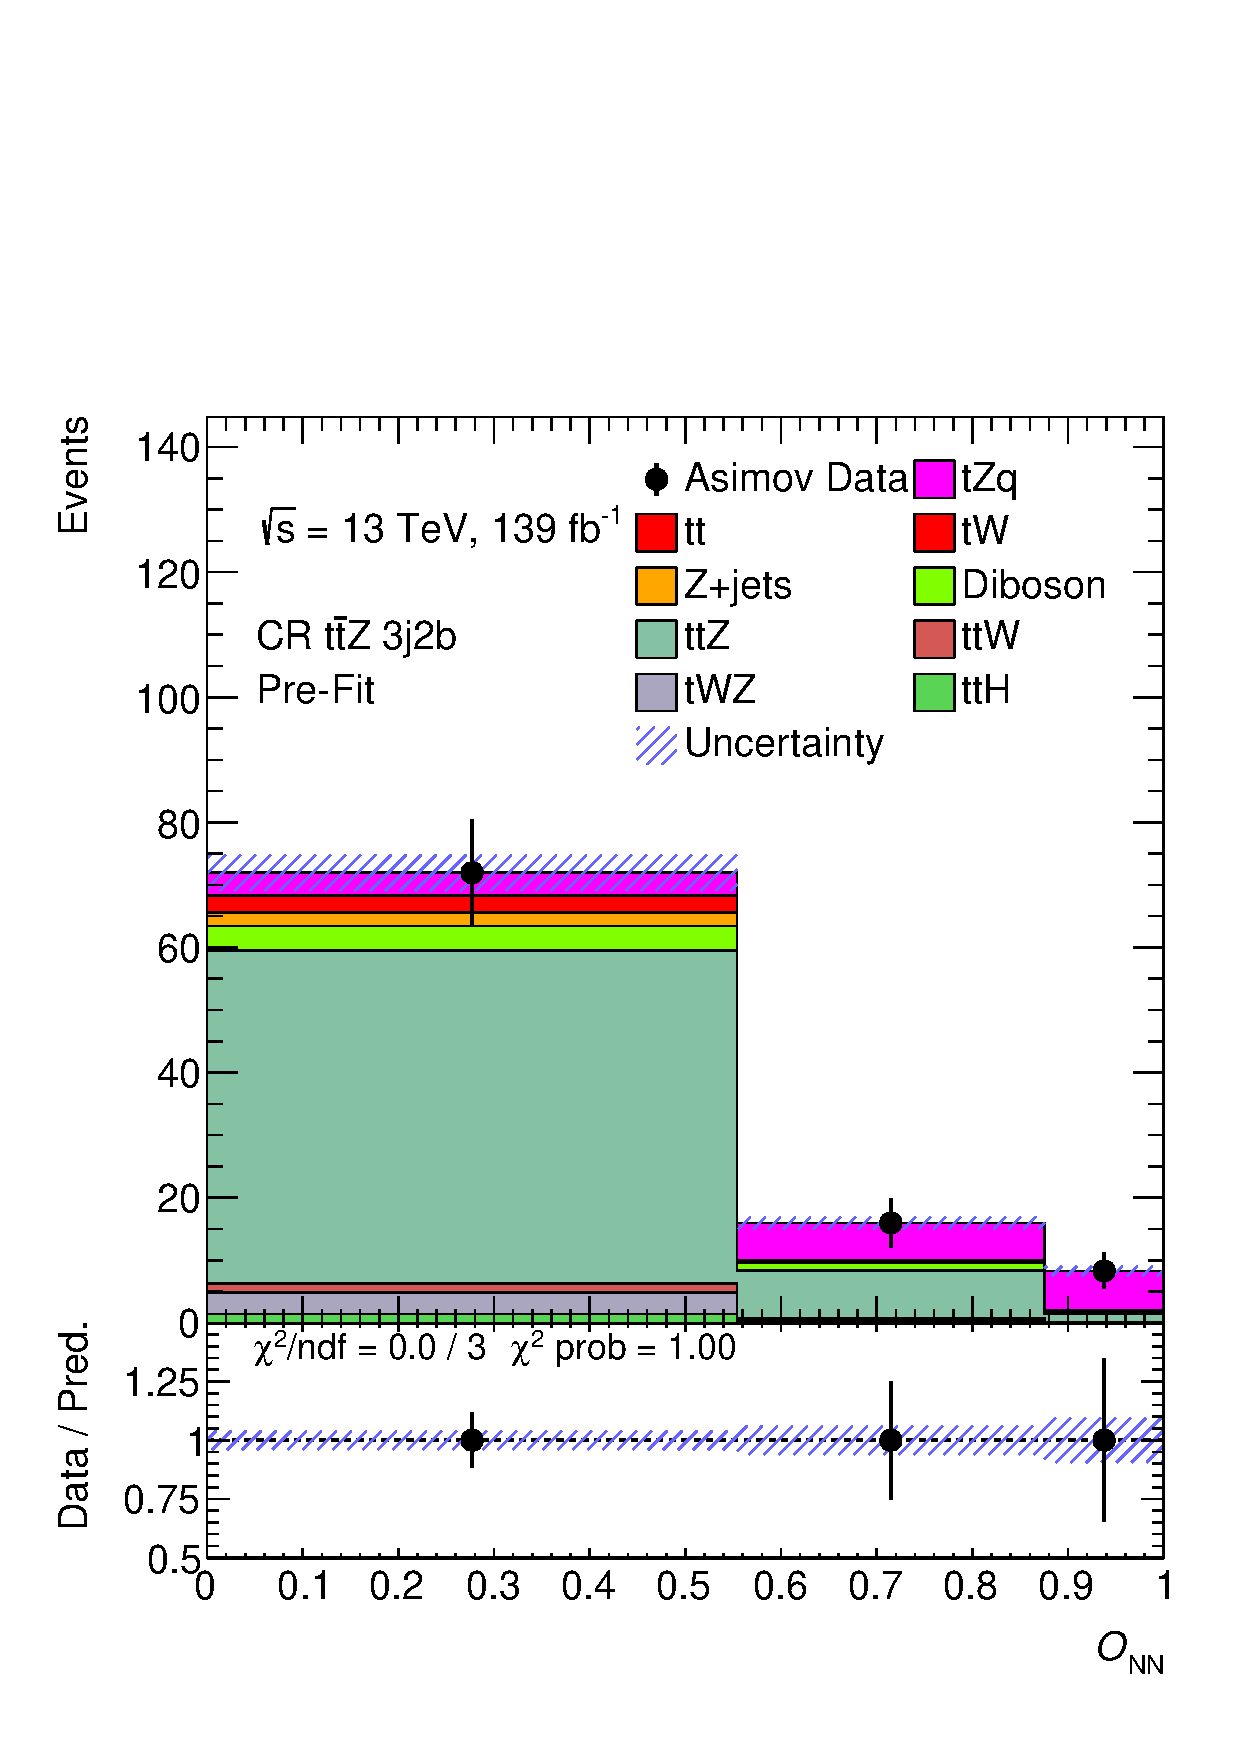
\includegraphics[width=\textwidth]{ubonn-thesis/Chapters/Chapters_07/Figure/Asmiov/CR_3j2b.pdf} 
  \end{subfigure}%%
  \newline
  \begin{subfigure}[b]{0.33\linewidth}
    \centering
    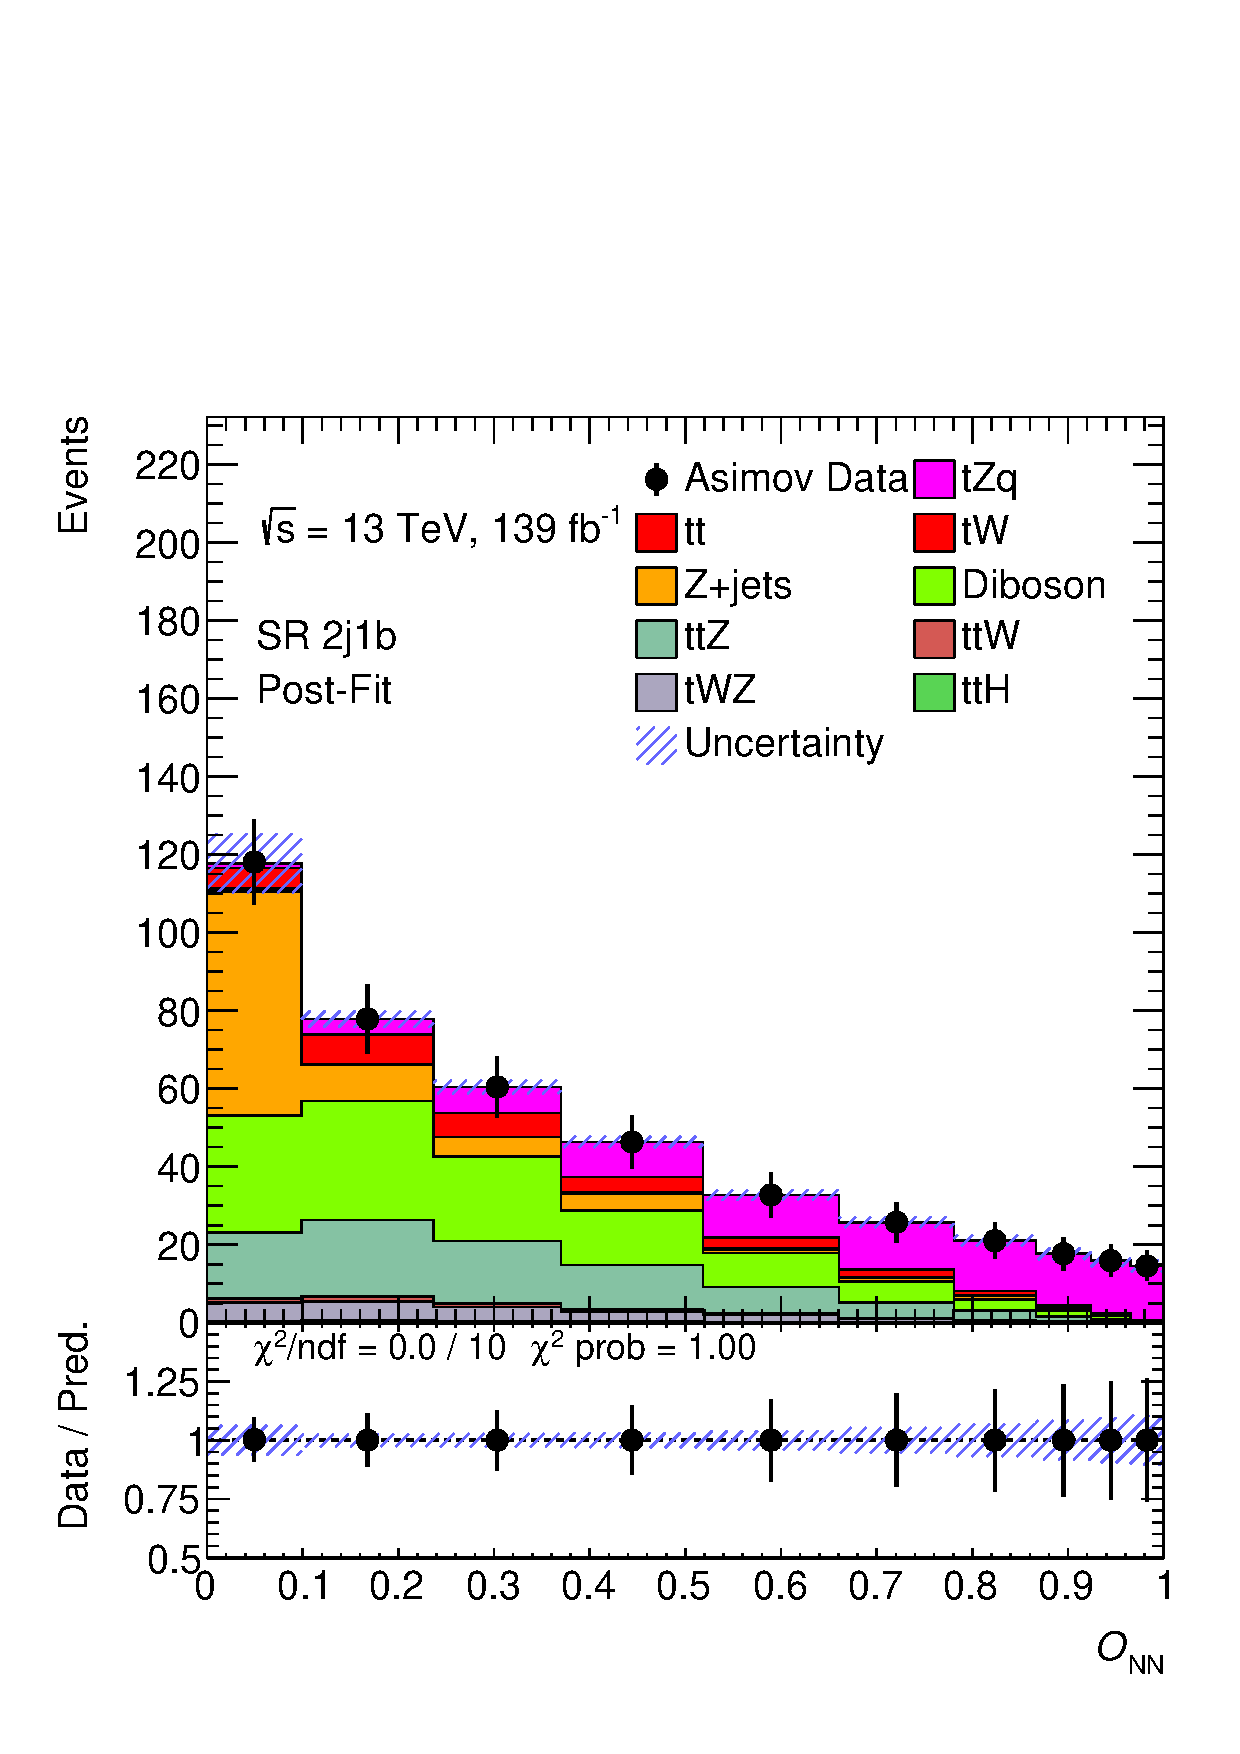
\includegraphics[width=\textwidth]{ubonn-thesis/Chapters/Chapters_07/Figure/Asmiov/SR_2j1b_postFit.pdf} 
  \end{subfigure} 
  \begin{subfigure}[b]{0.33\linewidth}
    \centering
    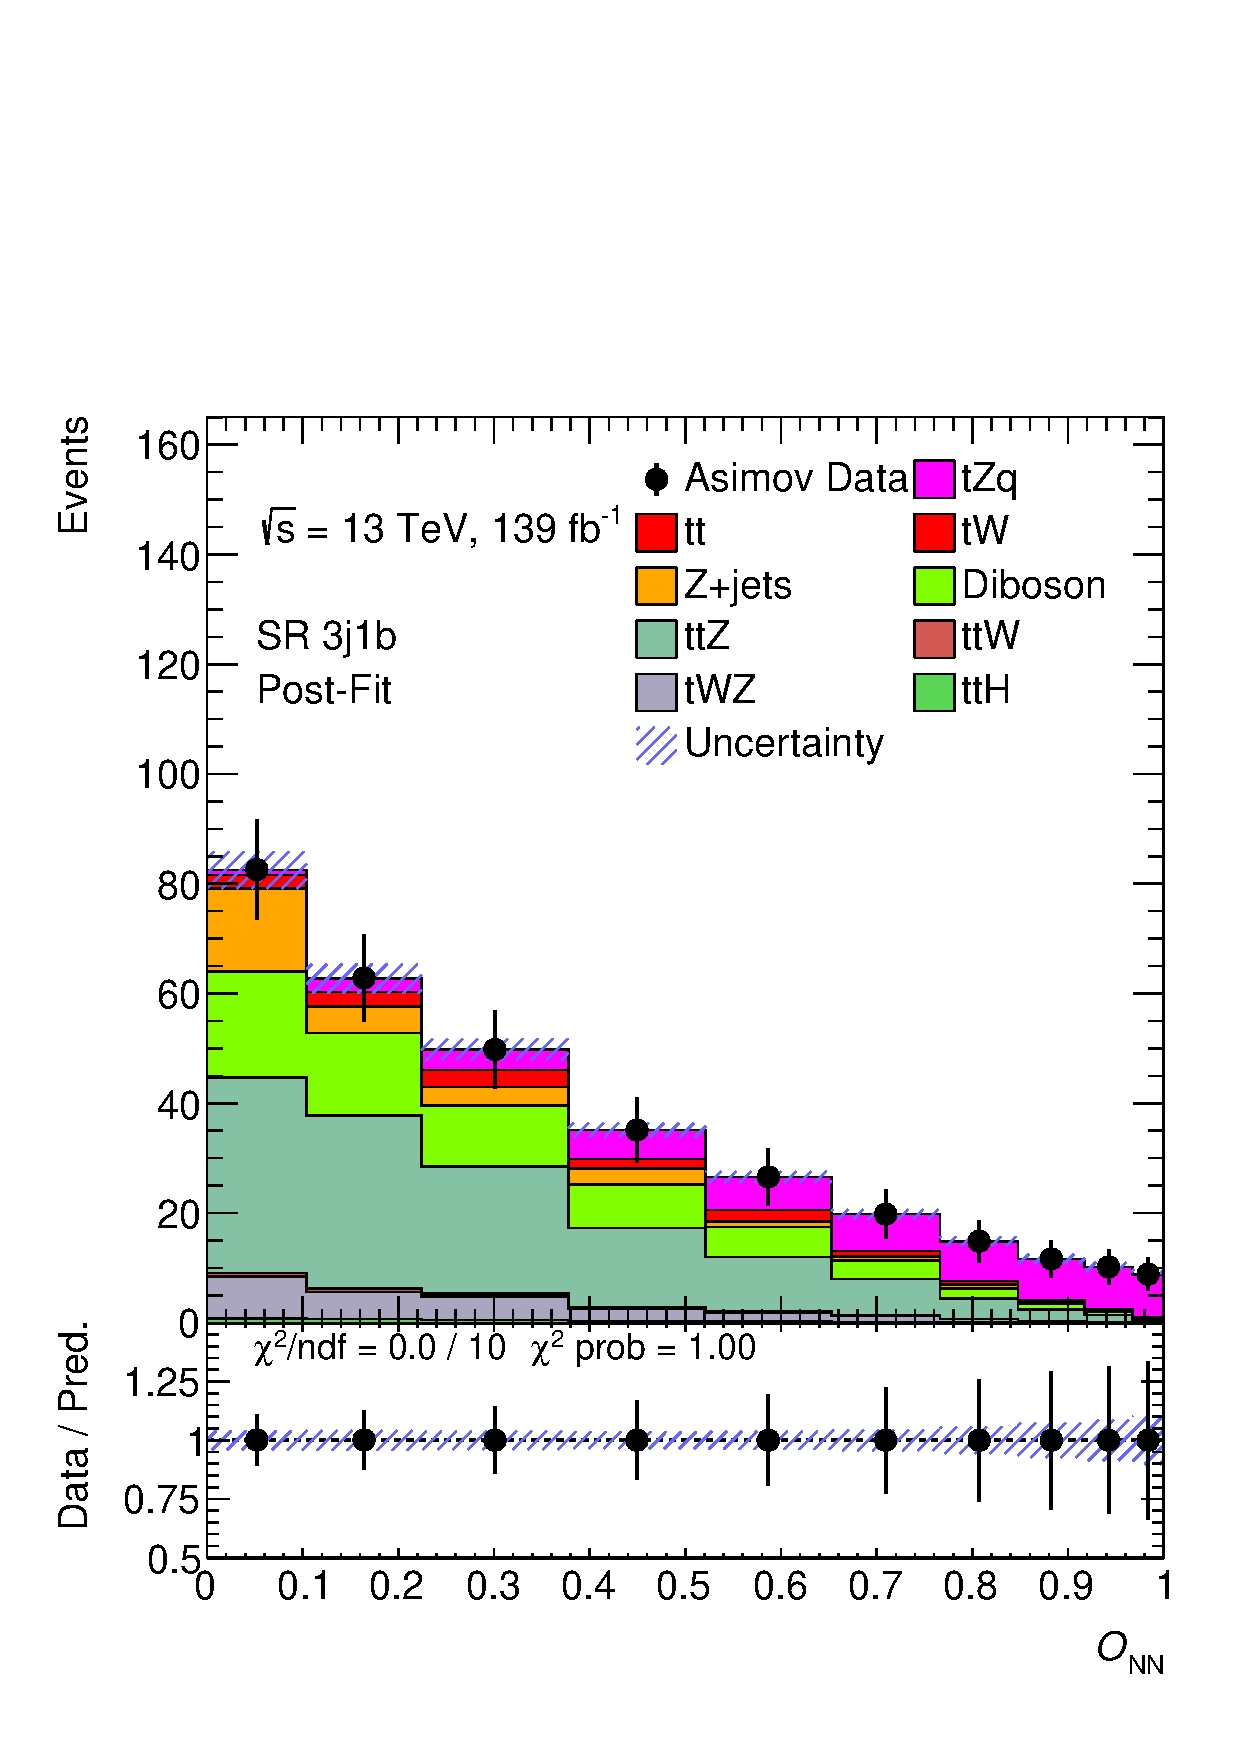
\includegraphics[width=\textwidth]{ubonn-thesis/Chapters/Chapters_07/Figure/Asmiov/SR_3j1b_postFit.pdf} 
  \end{subfigure}%% 
  \begin{subfigure}[b]{0.33\linewidth}
    \centering
    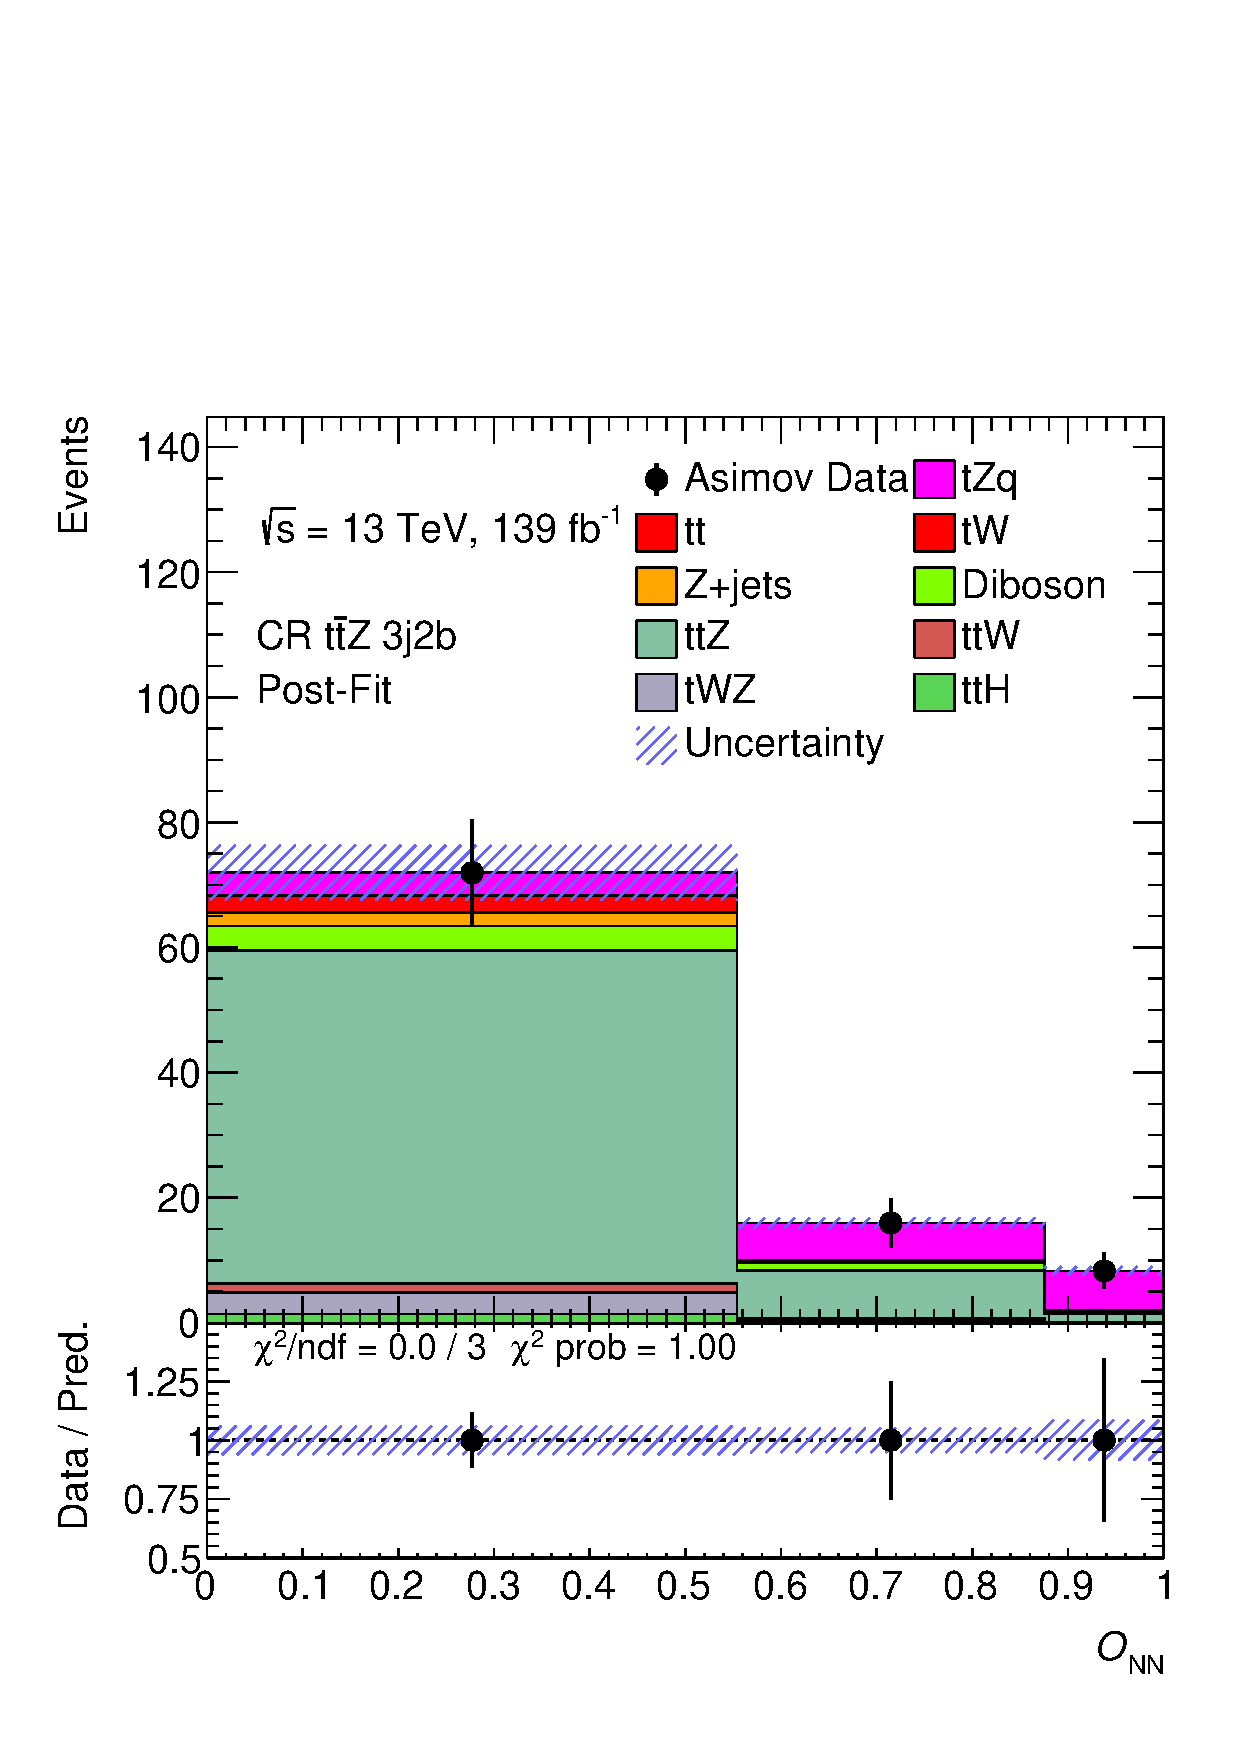
\includegraphics[width=\textwidth]{ubonn-thesis/Chapters/Chapters_07/Figure/Asmiov/CR_3j2b_postFit.pdf} 
  \end{subfigure} 
  \newline
  \begin{subfigure}[b]{0.33\linewidth}
    \centering
    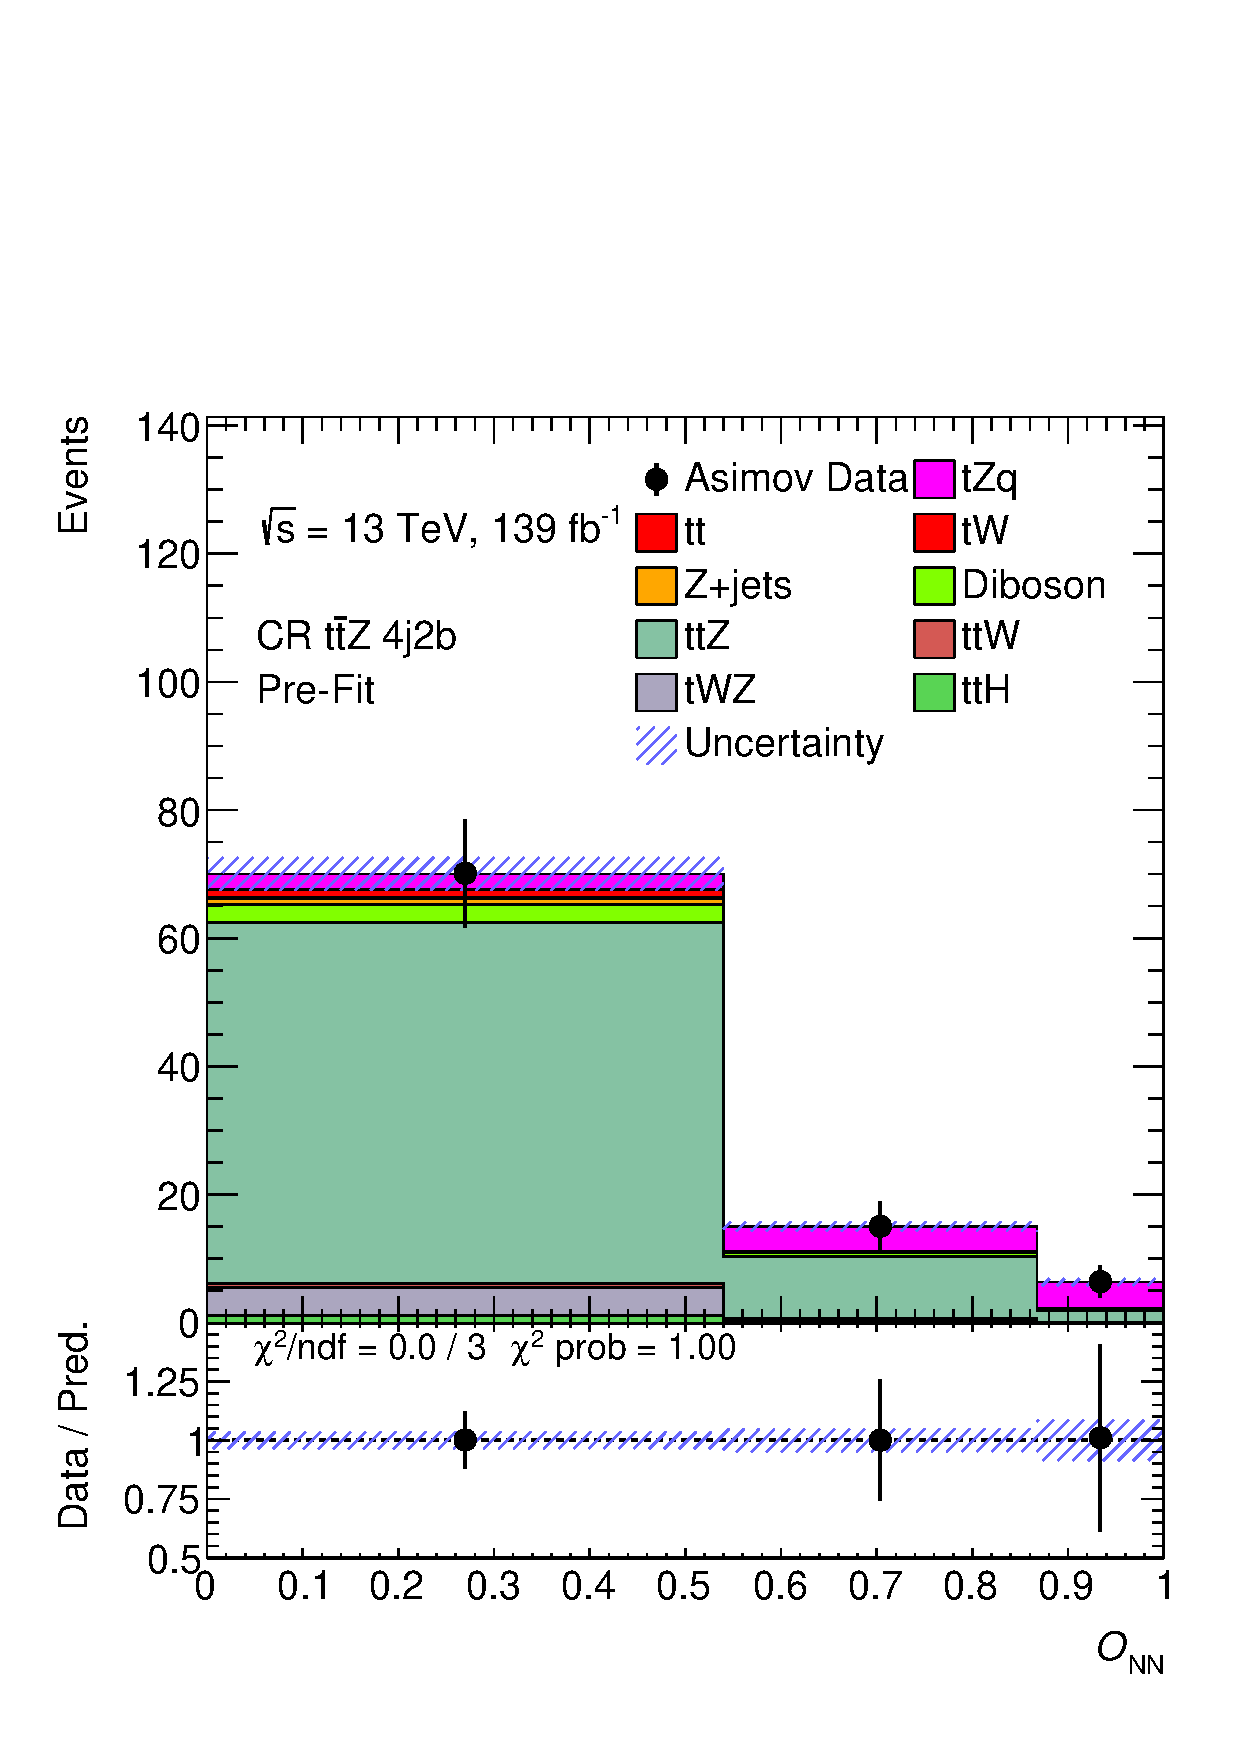
\includegraphics[width=\textwidth]{ubonn-thesis/Chapters/Chapters_07/Figure/Asmiov/CR_4j2b.pdf} 
  \end{subfigure} 
  \begin{subfigure}[b]{0.33\linewidth}
    \centering
    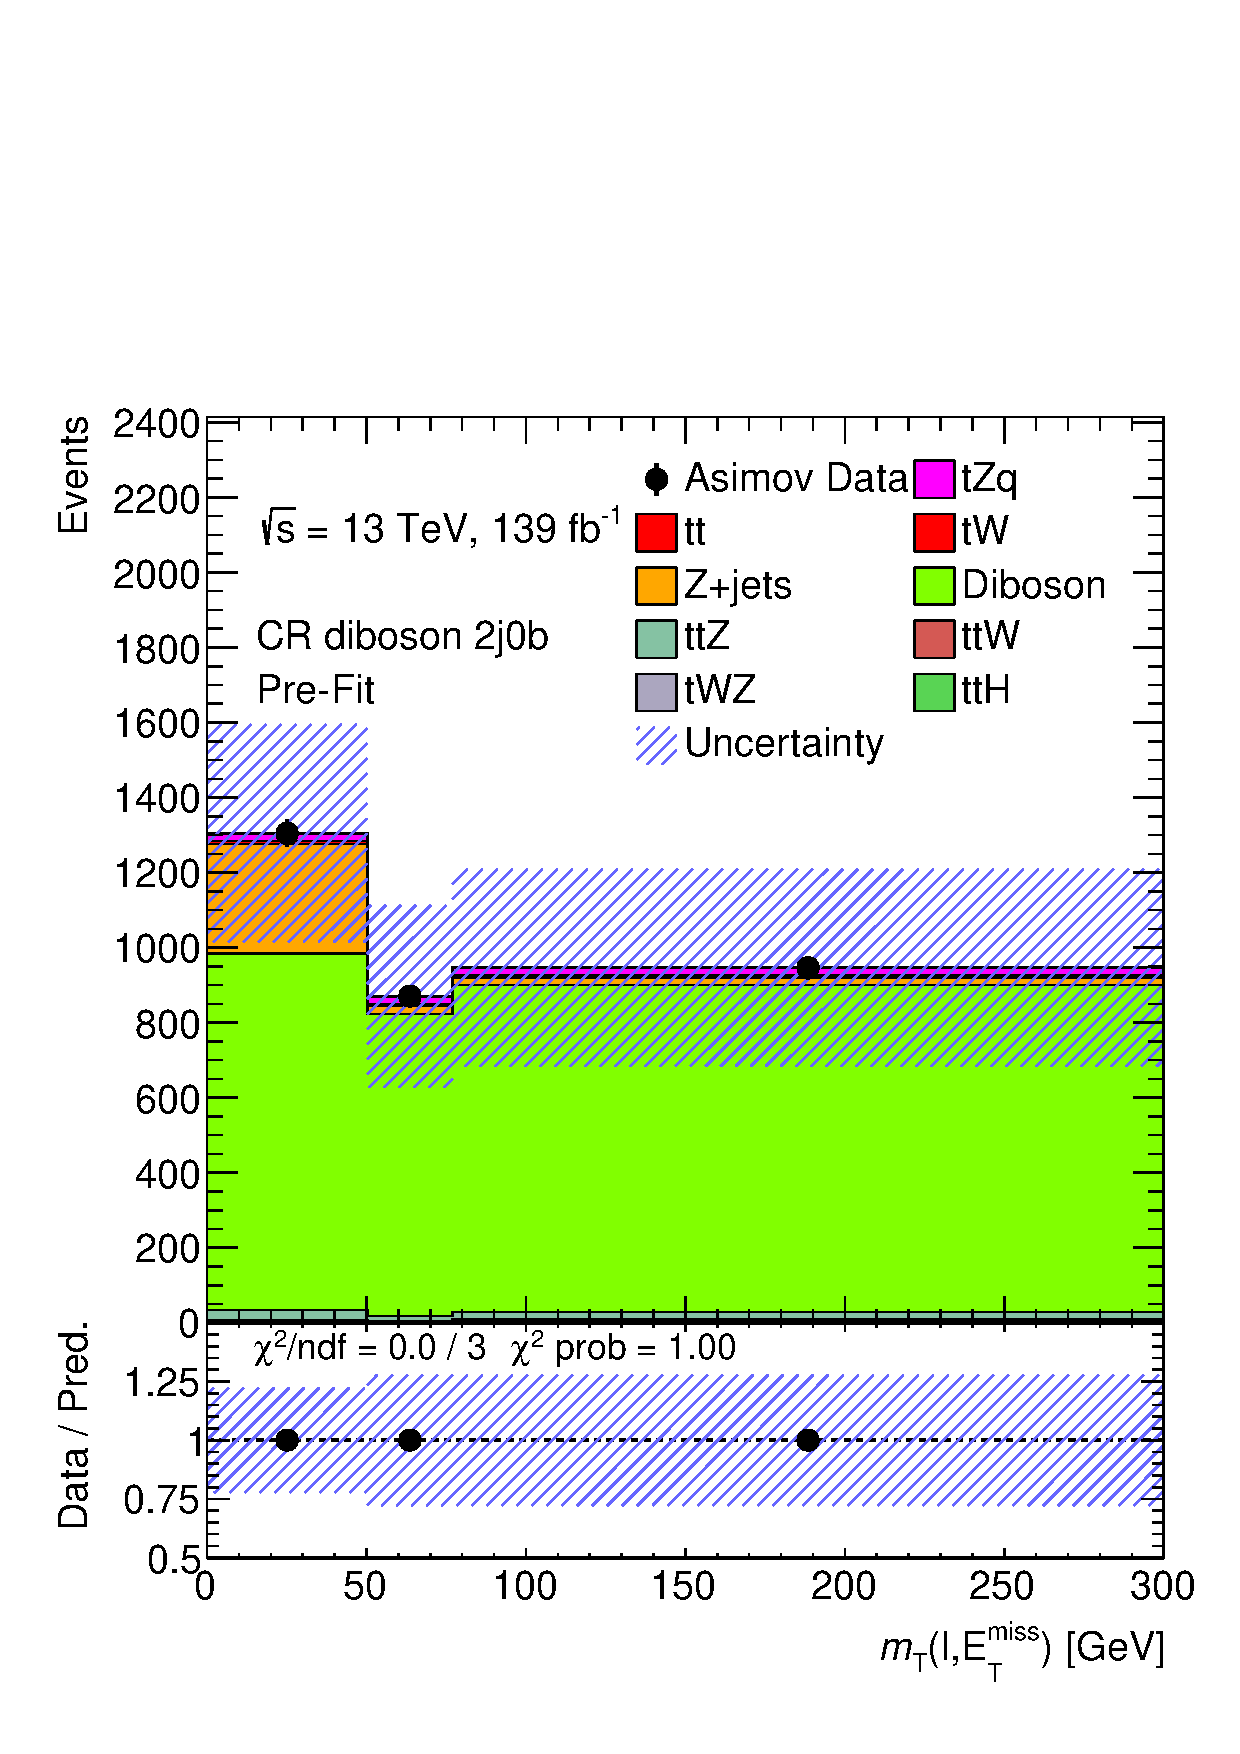
\includegraphics[width=\textwidth]{ubonn-thesis/Chapters/Chapters_07/Figure/Asmiov/CR_2j0b.pdf} 
  \end{subfigure}%% 
  \begin{subfigure}[b]{0.33\linewidth}
    \centering
    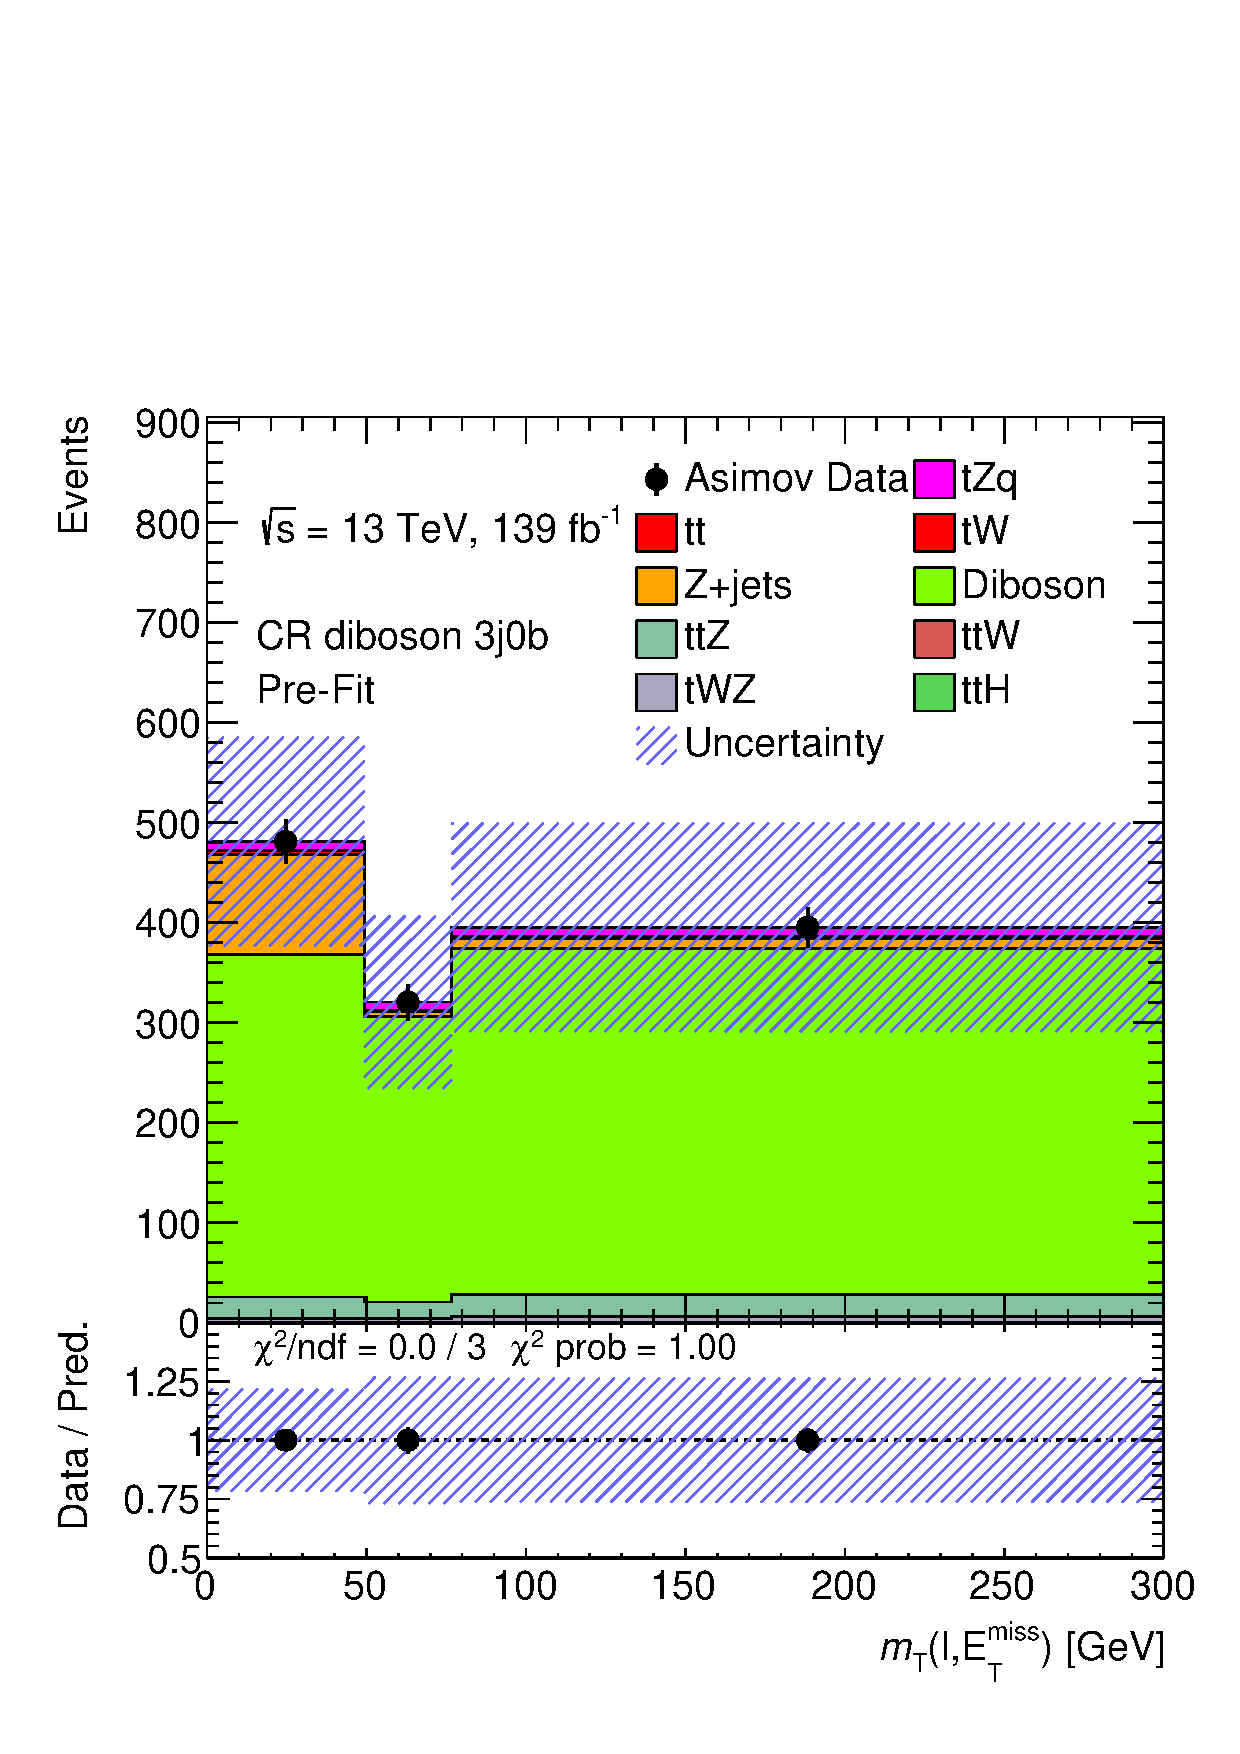
\includegraphics[width=\textwidth]{ubonn-thesis/Chapters/Chapters_07/Figure/Asmiov/CR_3j0b.pdf} 
  \end{subfigure} 
  \caption{ The pre-fit and post-fit distributions in the signal regions and control regions described in the table \ref{tab:fittedregions}. The black points show the blinded dataset. The error band includes the statistical and systematic uncertainties.}
  \label{fig:asimovfit1}
\end{figure}

\begin{figure}[!h] 
  \begin{subfigure}[b]{0.33\linewidth}
    \centering
    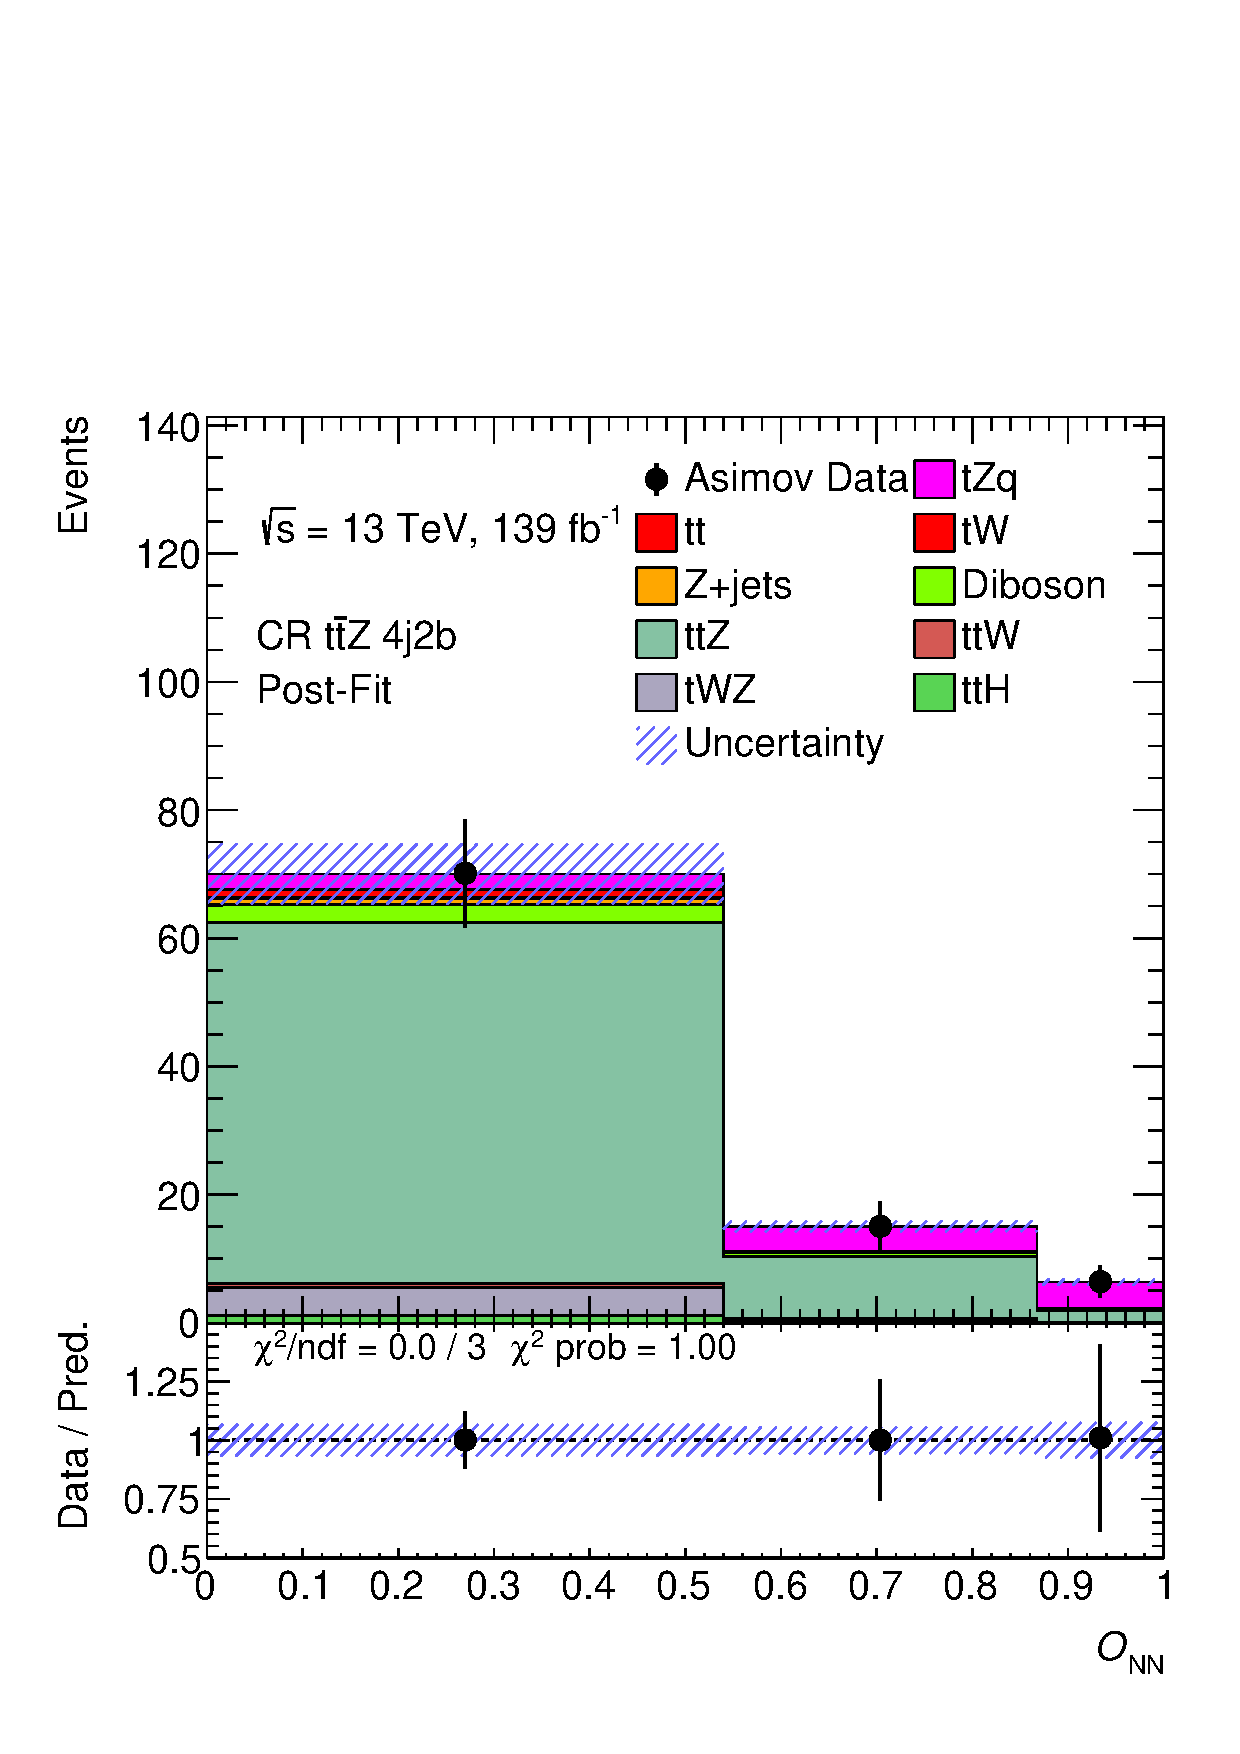
\includegraphics[width=\textwidth]{ubonn-thesis/Chapters/Chapters_07/Figure/Asmiov/CR_4j2b_postFit.pdf} 
    \caption{}
  \end{subfigure}%% 
  \begin{subfigure}[b]{0.33\linewidth}
    \centering
    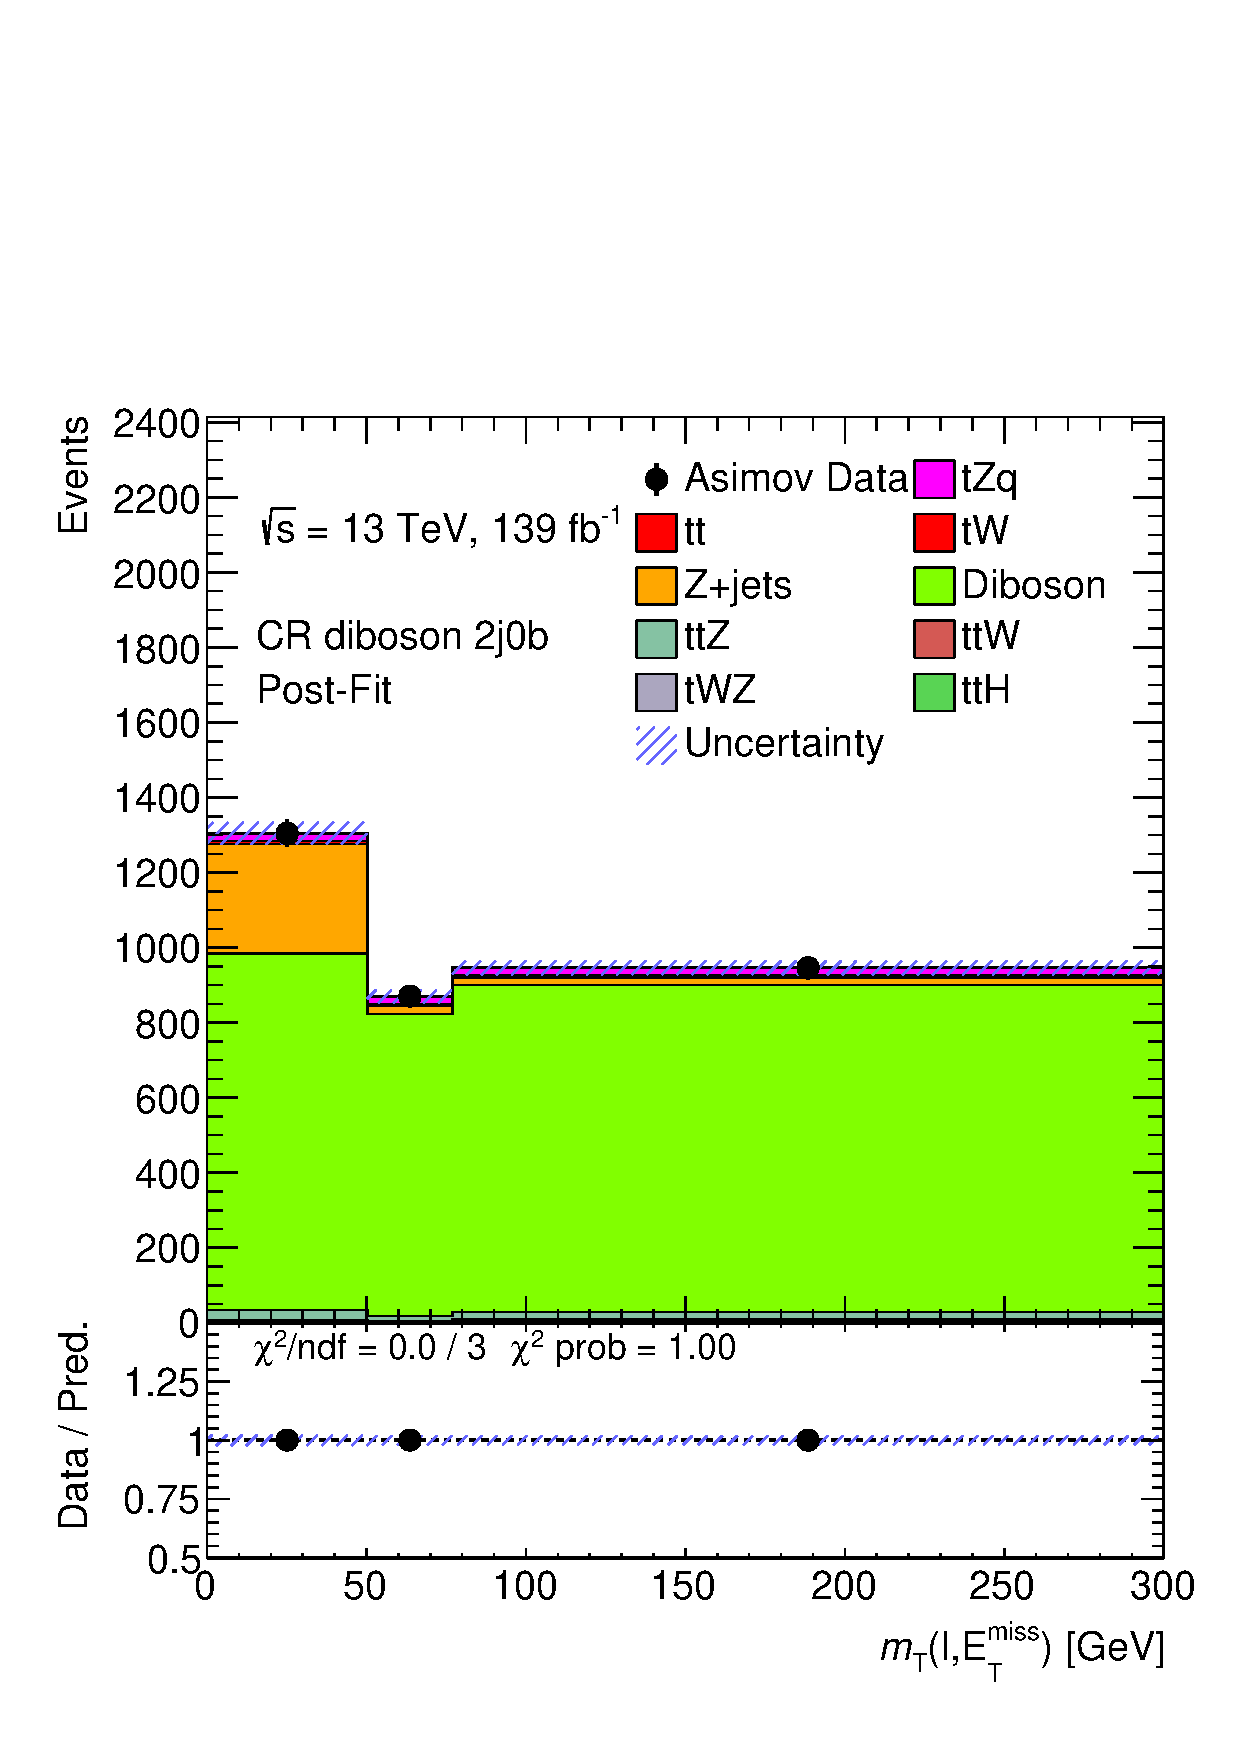
\includegraphics[width=\textwidth]{ubonn-thesis/Chapters/Chapters_07/Figure/Asmiov/CR_2j0b_postFit.pdf} 
    \caption{}
  \end{subfigure} 
  \begin{subfigure}[b]{0.33\linewidth}
    \centering
    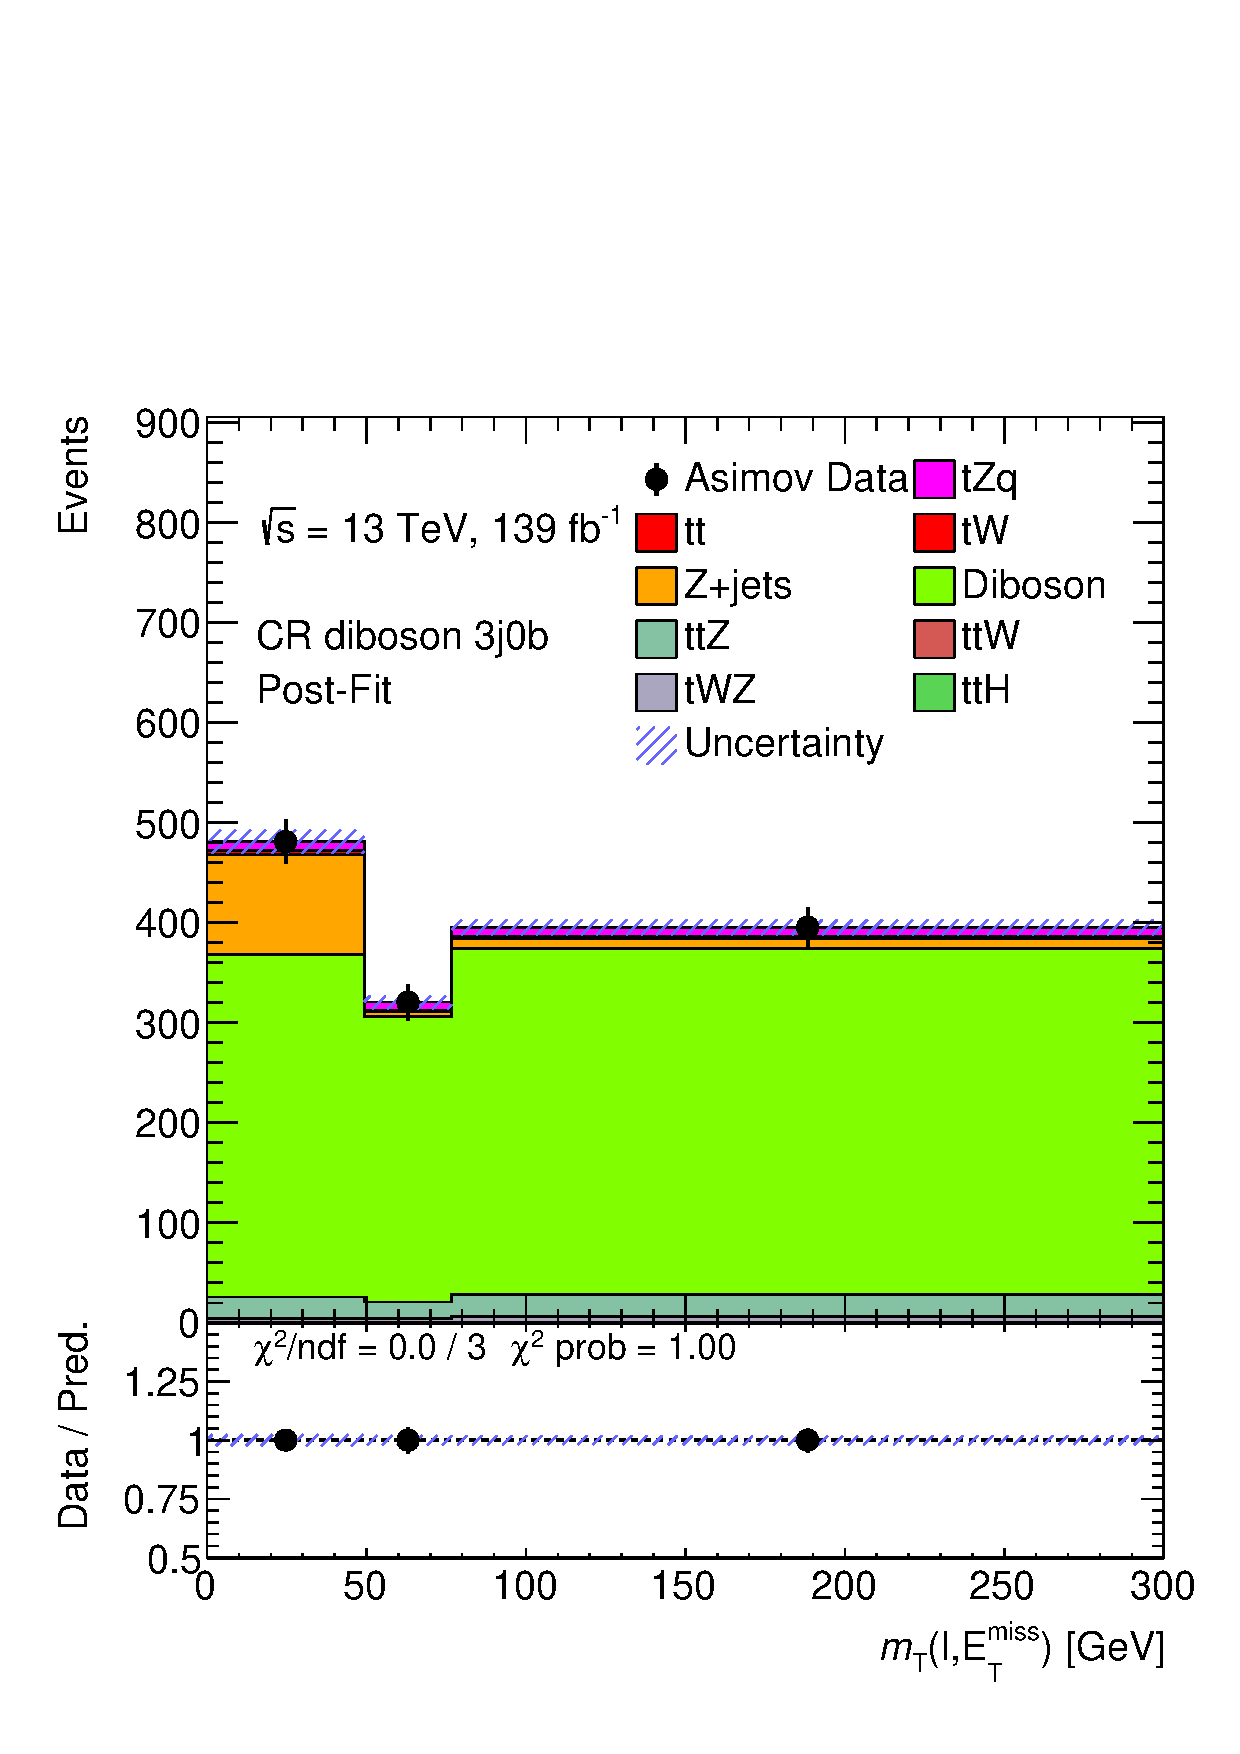
\includegraphics[width=\textwidth]{ubonn-thesis/Chapters/Chapters_07/Figure/Asmiov/CR_3j0b_postFit.pdf} 
    \caption{}
  \end{subfigure}%%
  \newline
  \centering
  \begin{subfigure}[b]{0.33\linewidth}
    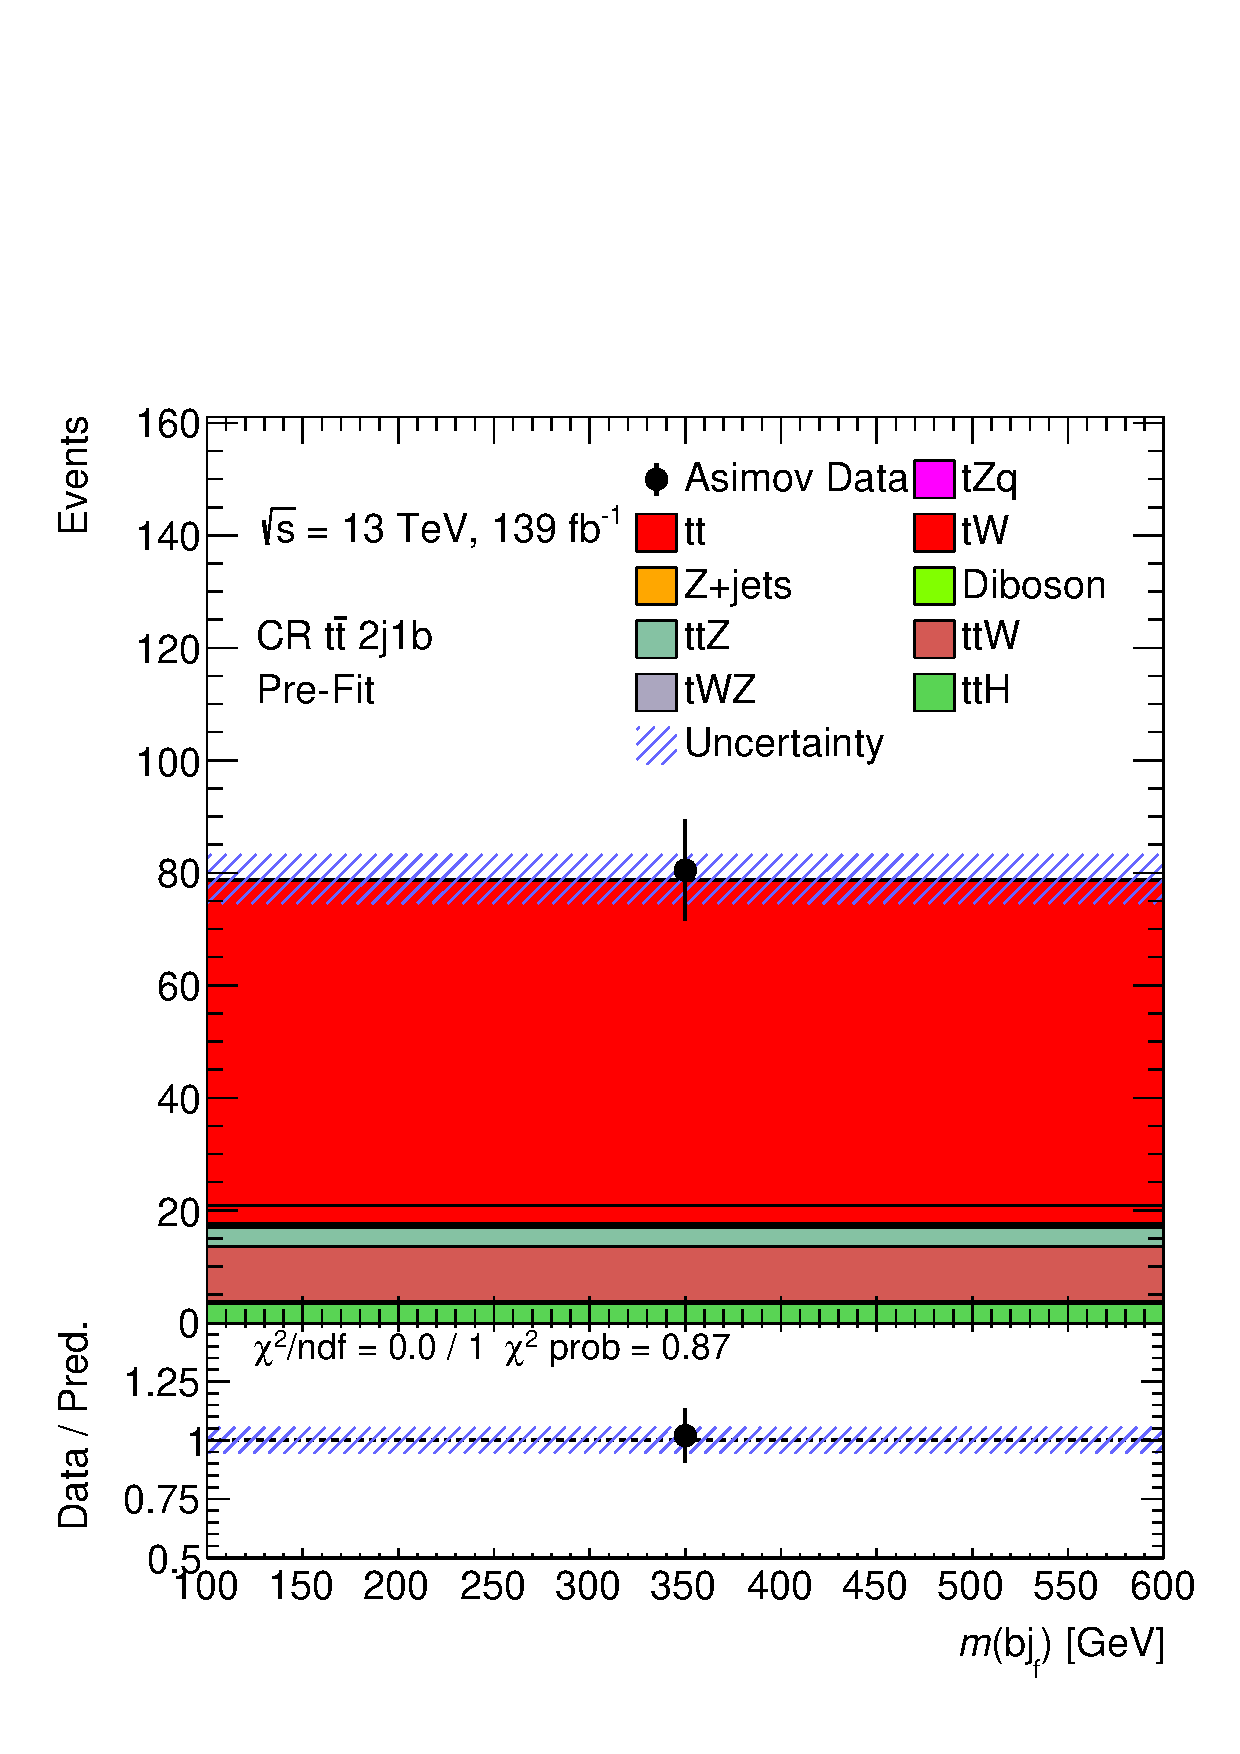
\includegraphics[width=\textwidth]{ubonn-thesis/Chapters/Chapters_07/Figure/Asmiov/CR_2j1b.pdf} 
    \caption{}
  \end{subfigure} 
  \centering
  \begin{subfigure}[b]{0.33\linewidth}
    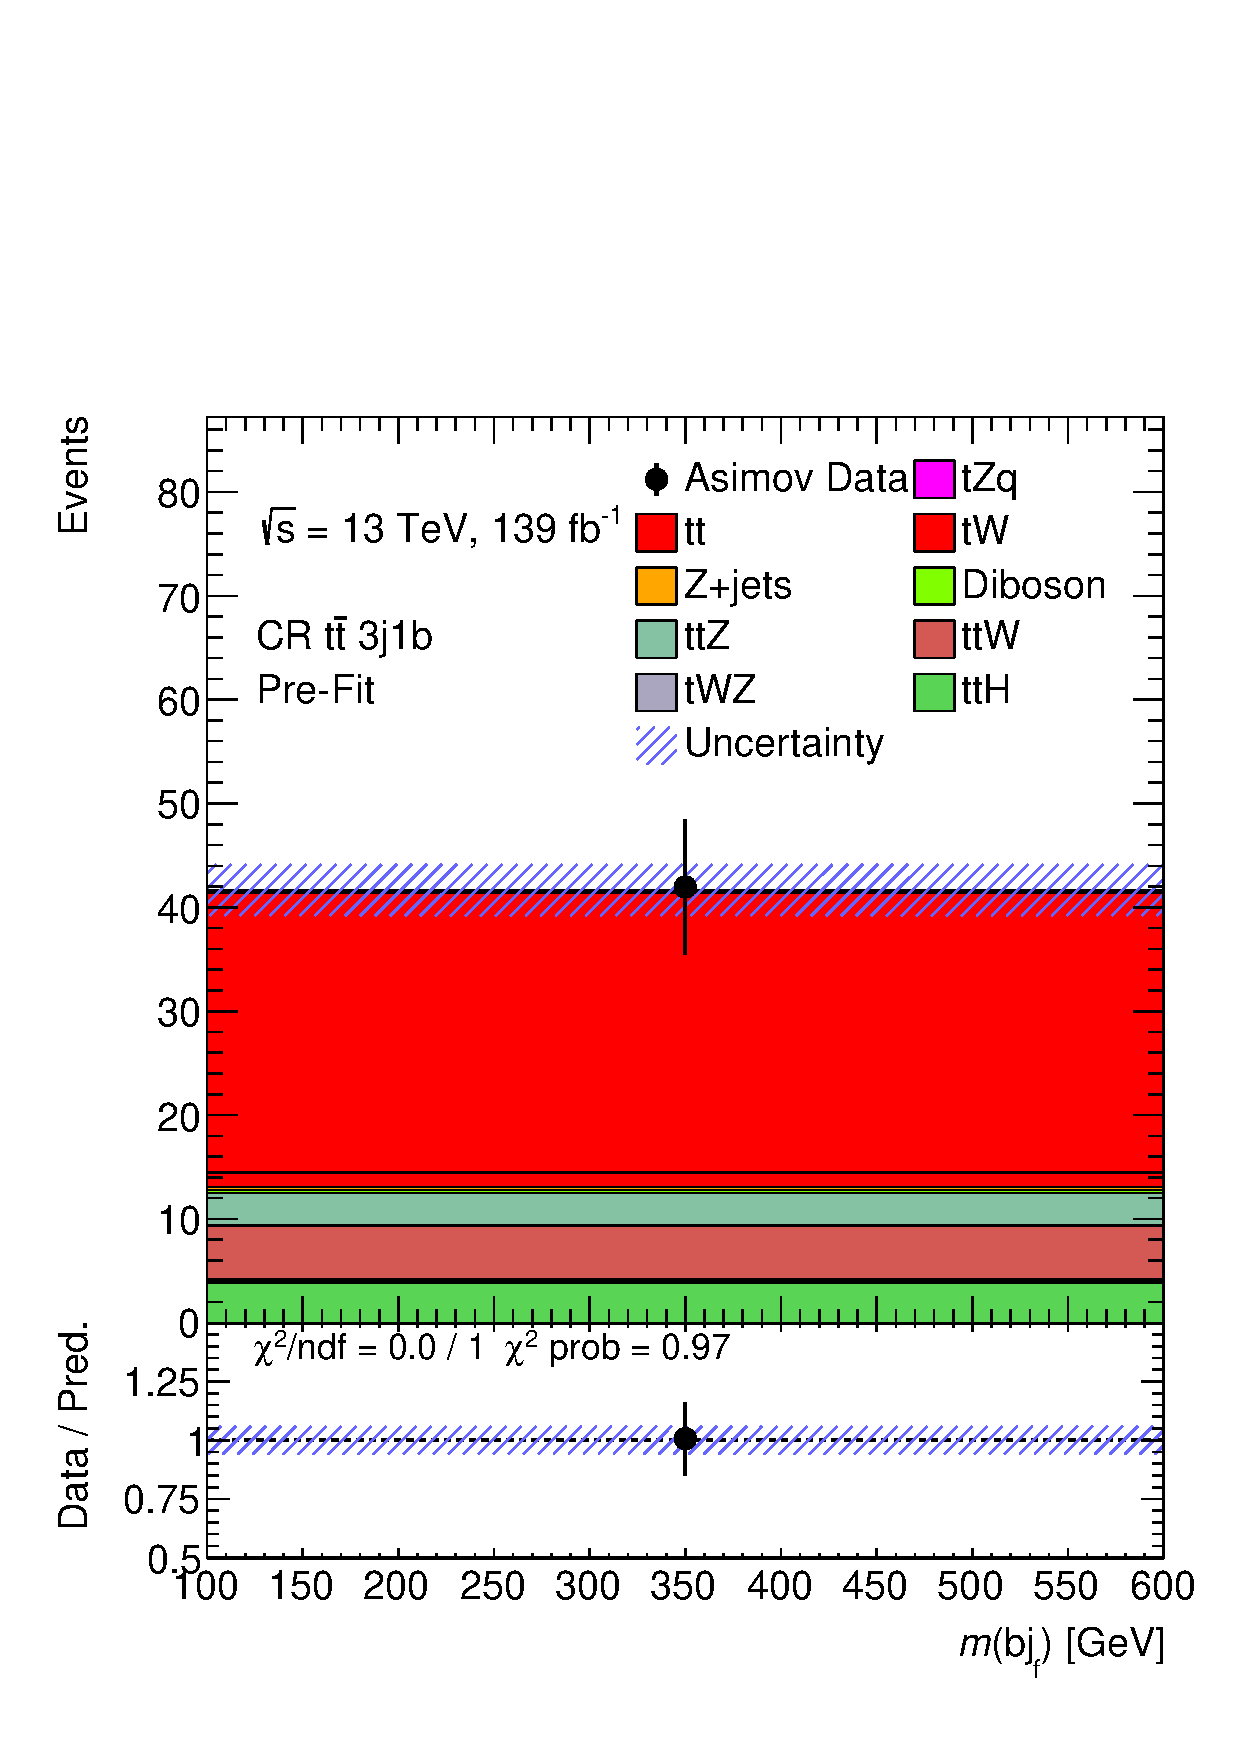
\includegraphics[width=\textwidth]{ubonn-thesis/Chapters/Chapters_07/Figure/Asmiov/CR_3j1b.pdf} 
    \caption{}
  \end{subfigure}%% 
  \newline
  \hspace*{-1.5cm}
  \begin{subfigure}[b]{0.33\linewidth}
   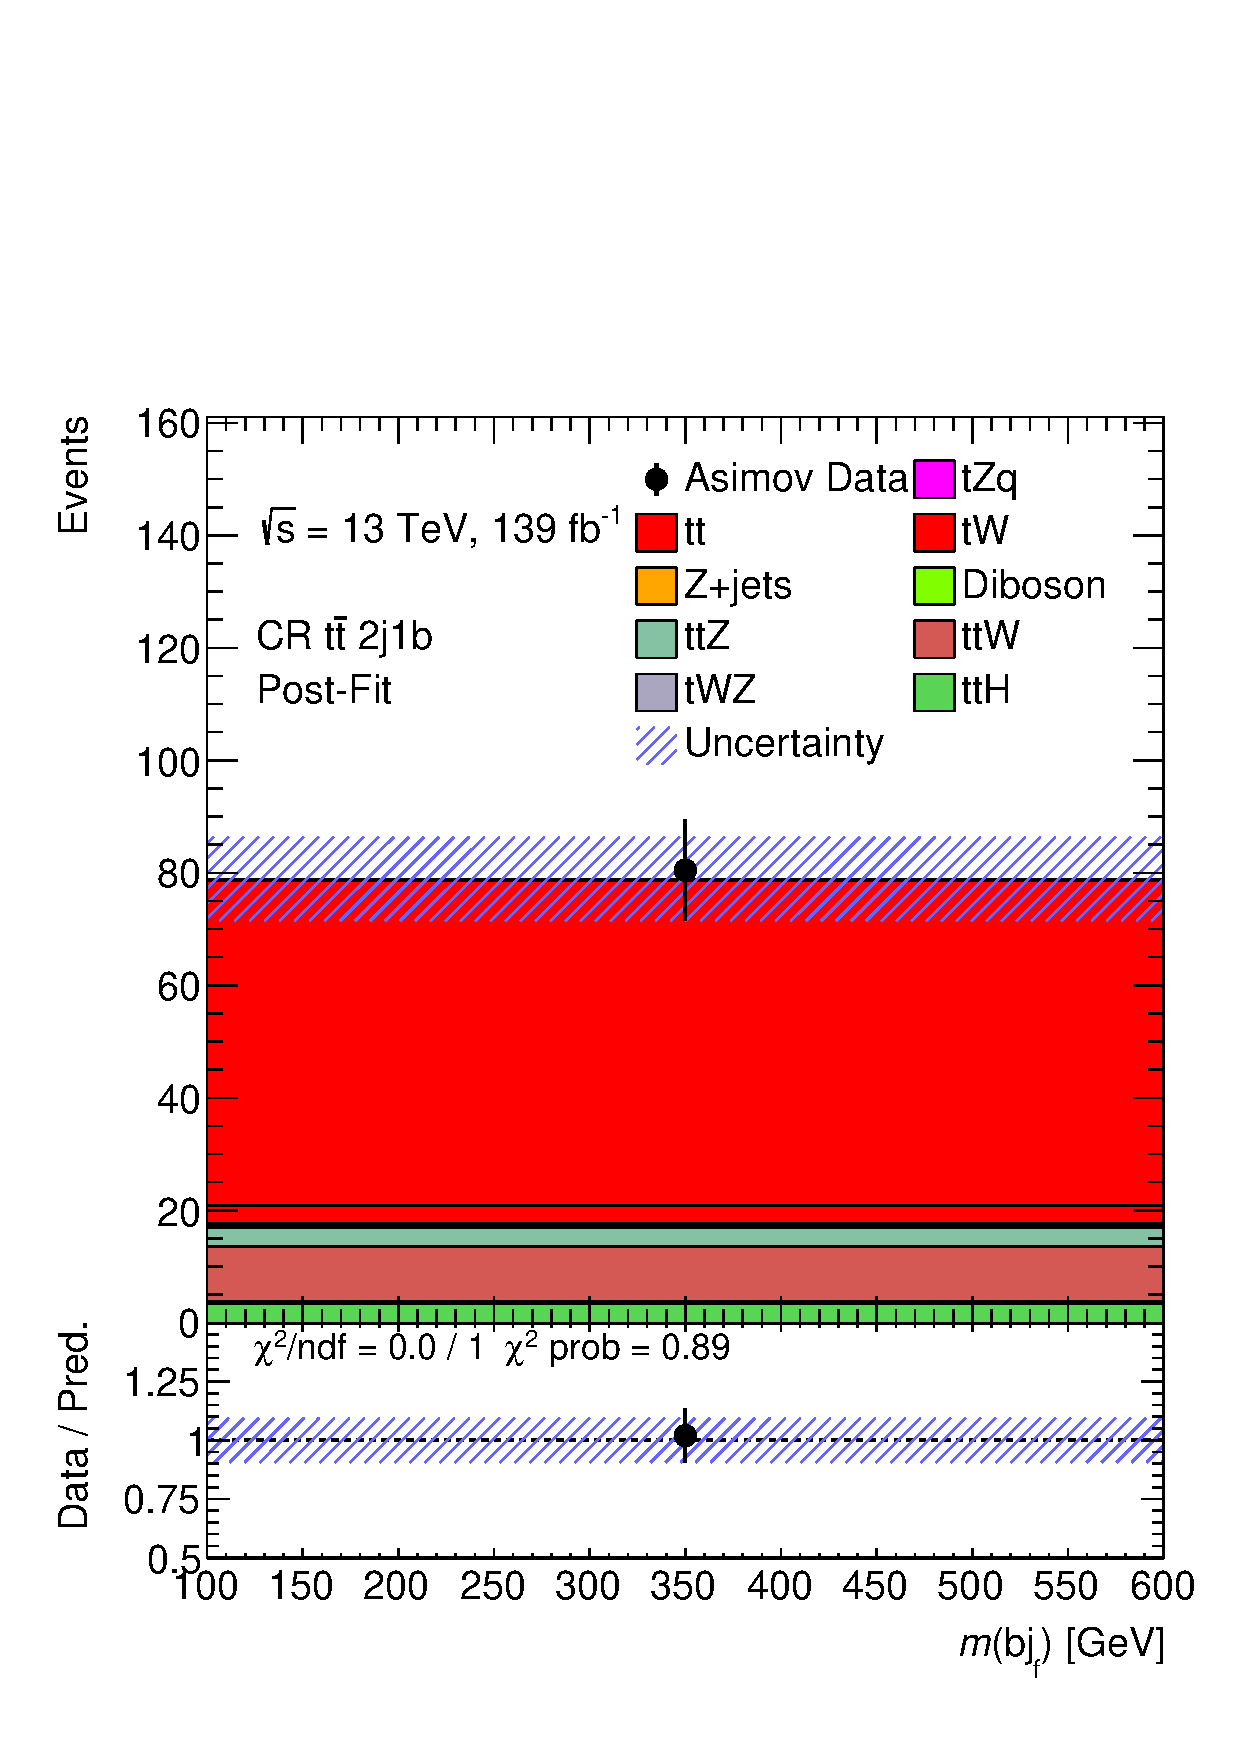
\includegraphics[width=\textwidth]{ubonn-thesis/Chapters/Chapters_07/Figure/Asmiov/CR_2j1b_postFit.pdf} 
    \caption{}
  \end{subfigure} 
  \centering
  \begin{subfigure}[b]{0.33\linewidth}
  %\hspace*{-1.0cm}
    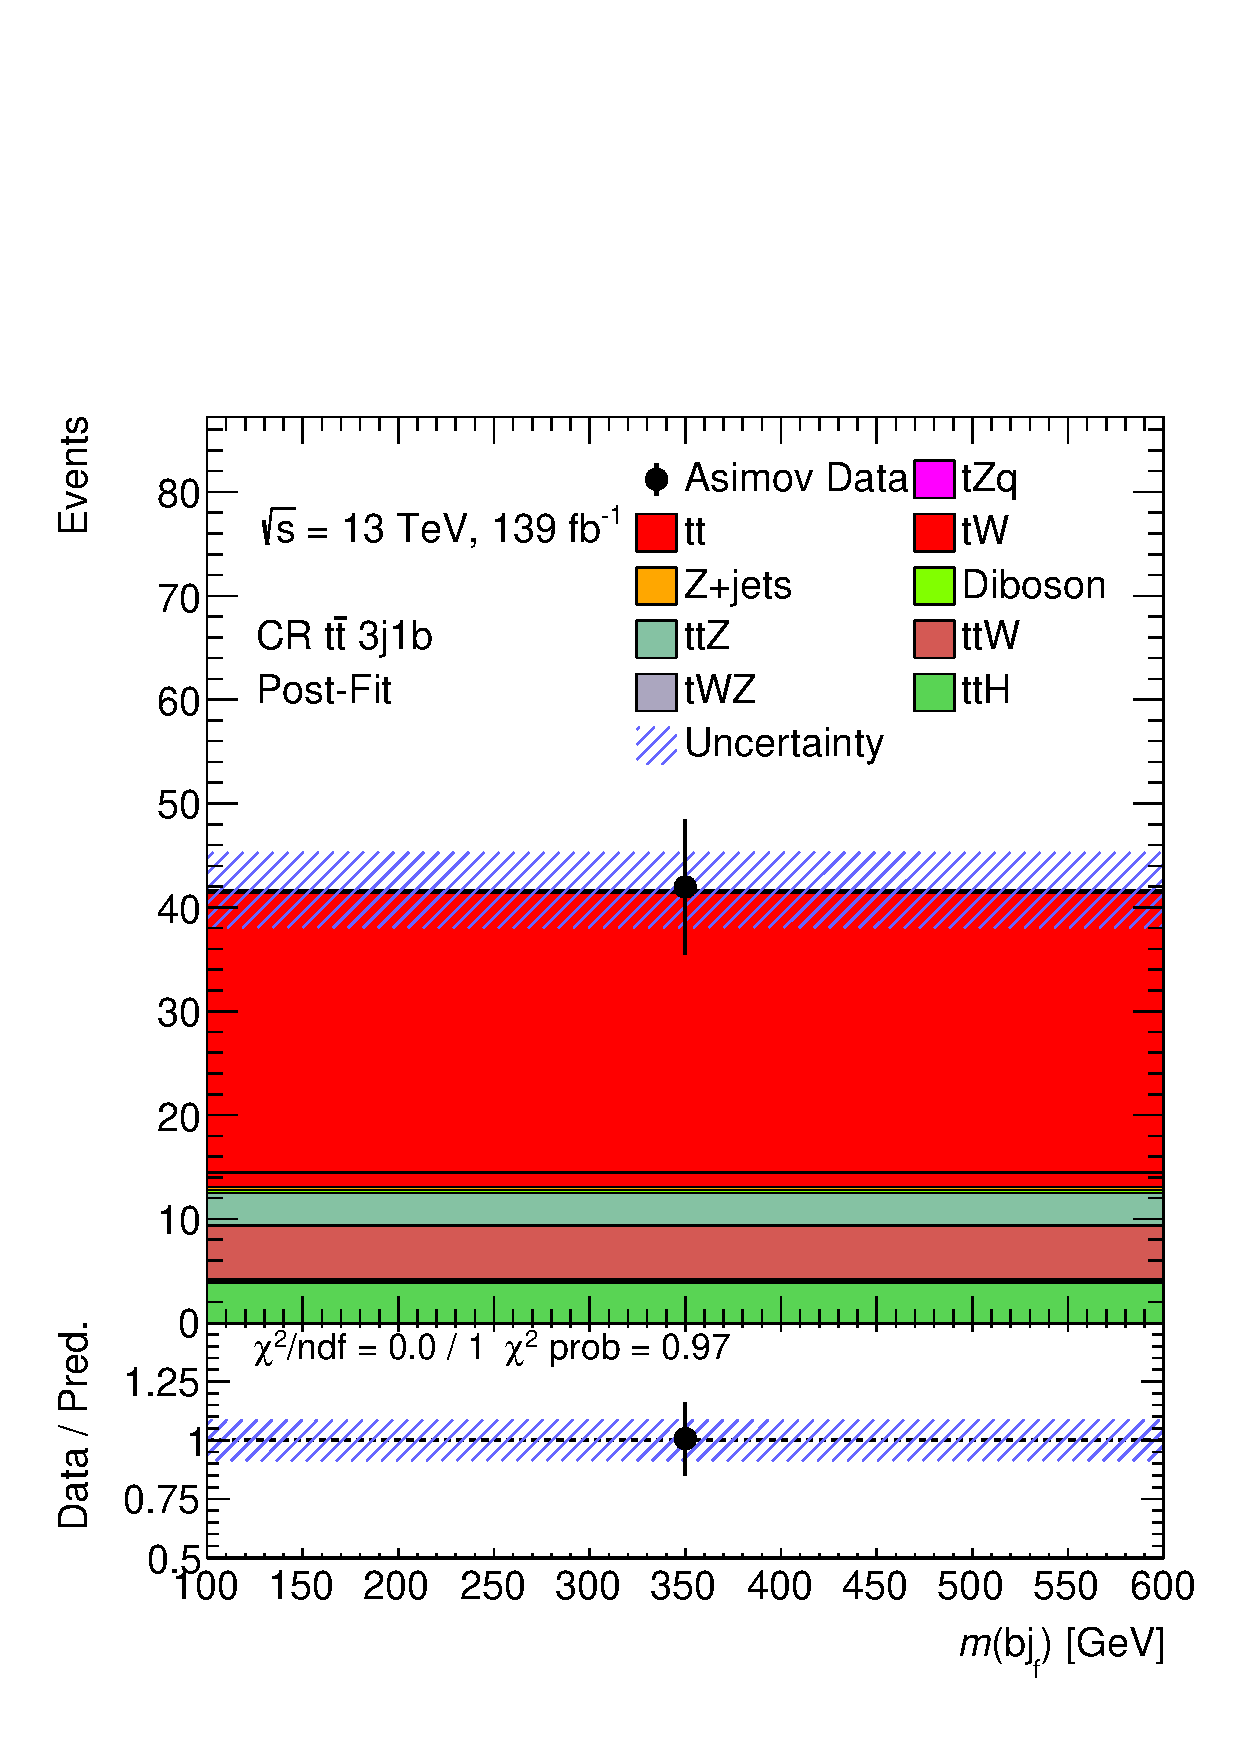
\includegraphics[width=\textwidth]{ubonn-thesis/Chapters/Chapters_07/Figure/Asmiov/CR_3j1b_postFit.pdf}
   \caption{}
  \end{subfigure}%% 
  \caption{Pre-fit and post-fit distributions in the signal regions and control regions described in the table \ref{tab:fittedregions}. The black points show the blinded dataset. The error band includes the statistical and systematic uncertainties.}
  \label{fig:asimovfit2}
  \end{figure}

\newpage

\newpage

\begin{table}[h!]
     \centering
      {\footnotesize \begin{tabular}{@{} *4l  @{}}
      \toprule
       Region & Distribution & Additional Info \\
     \midrule
      SR 2j1b & $m_{bj_{f}}$ & {--}\\[0.2ex]
      SR 3j1b & $m_{bj_{f}}$ & {--}\\[0.2ex]
      CR diboson 2j0b & $m_{T}(\ell,E_{T}^{miss})$ & {--}\\[0.2ex]
      CR diboson 3j0b & $m_{T}(\ell,E_{T}^{miss})$ & {--}\\[0.2ex]
      CR $t\Bar{t}$ 2j1b & $m_{bj_{f}}$ & Single bin \\[0.2ex]
      CR $t\Bar{t}$ 3j1b & $m_{bj_{f}}$ & Single bin \\[0.2ex]
      CR $t\Bar{t}Z$ 3j2b & $m_{bj_{f}}$ & {--}\\[0.2ex]
      CR $t\Bar{t}Z$ 4j2b & $m_{bj_{f}}$ & {--}\\[0.2ex]
      \bottomrule
 \end{tabular}}
 \caption{Overview of the regions included in the new fit without neural network training}
 \label{tab:newfittedregions}
 \end{table}
 
 
 \begin{figure}[!h] 
  \begin{subfigure}[b]{0.49\linewidth}
    \centering
    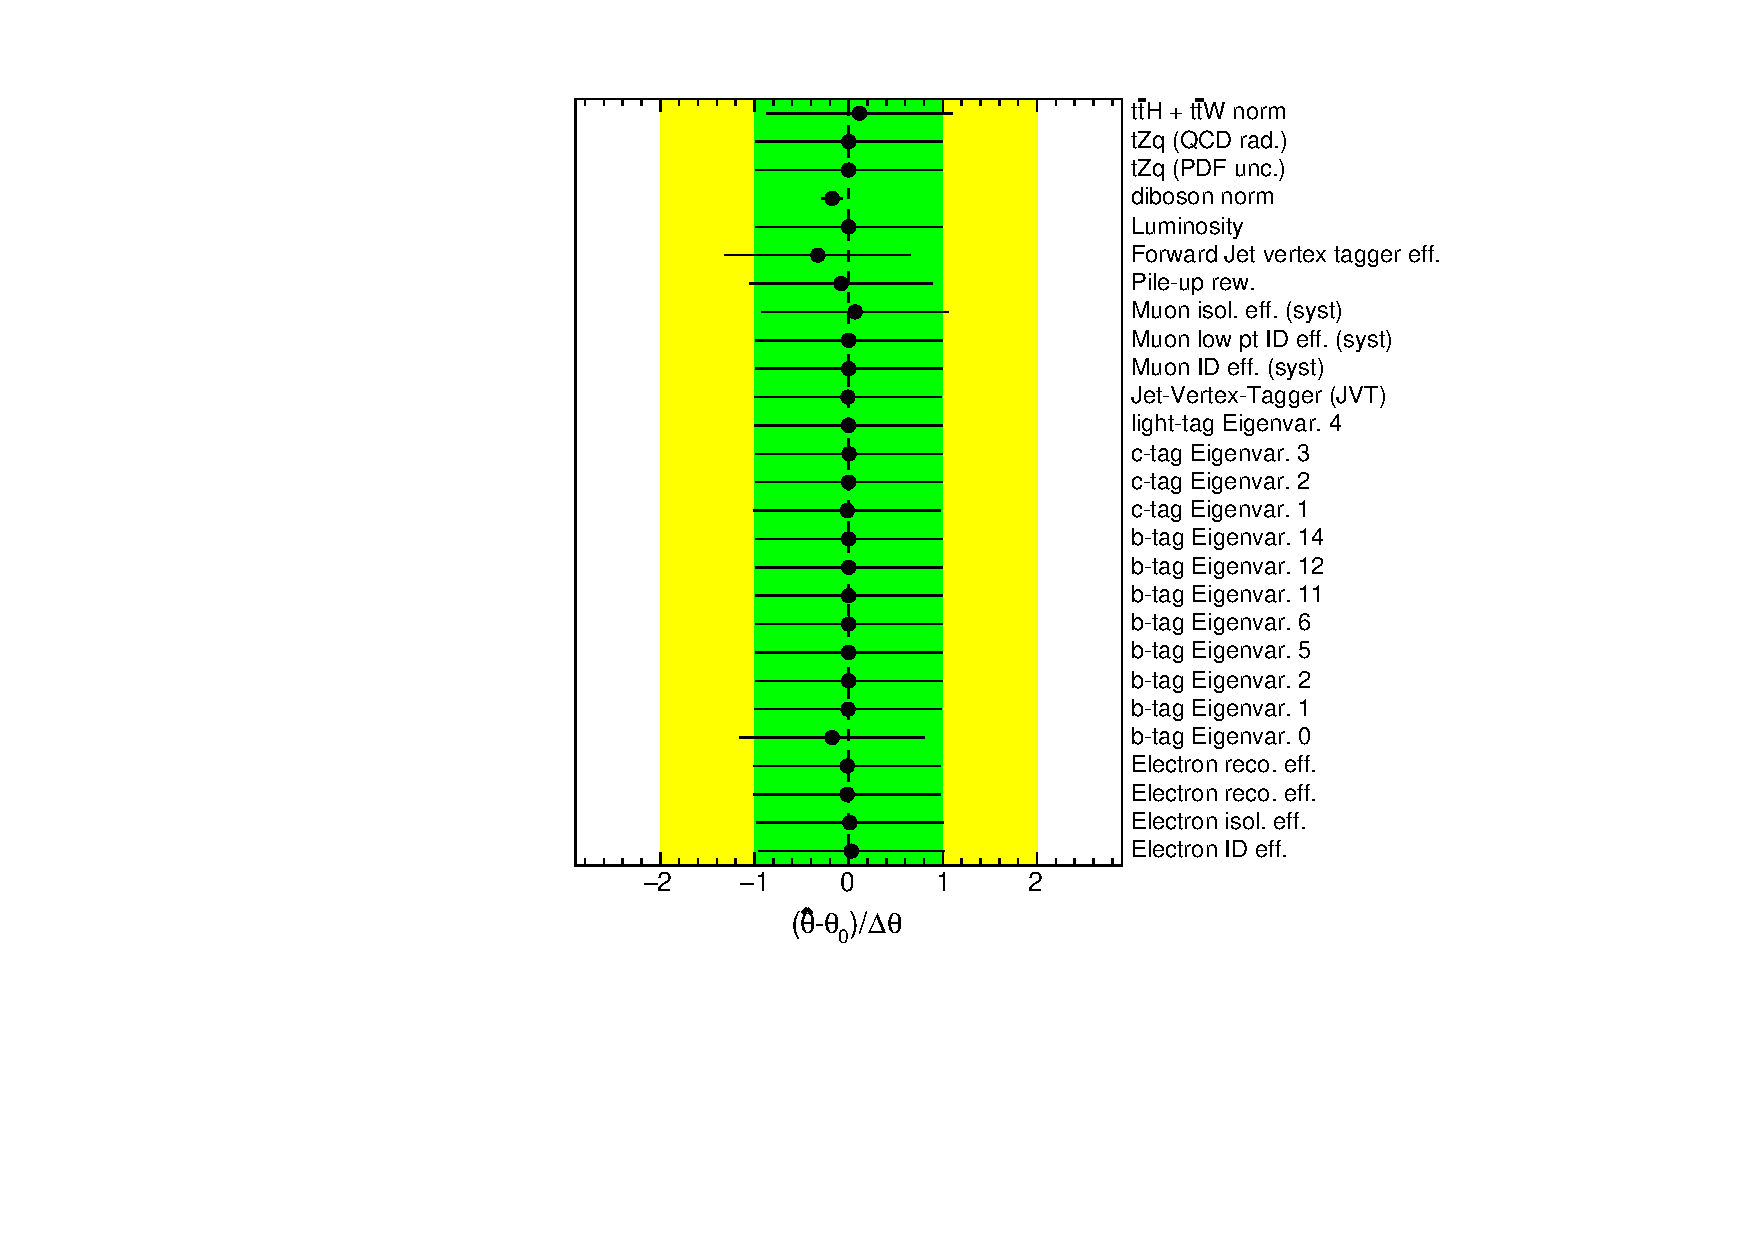
\includegraphics[width=1.24\textwidth]{ubonn-thesis/Chapters/Chapters_08/appendix/data/NuisPar.pdf}
    \caption{}
    \label{fig:newvpull}
  \end{subfigure}%% 
  \begin{subfigure}[b]{0.49\linewidth}
    \centering
    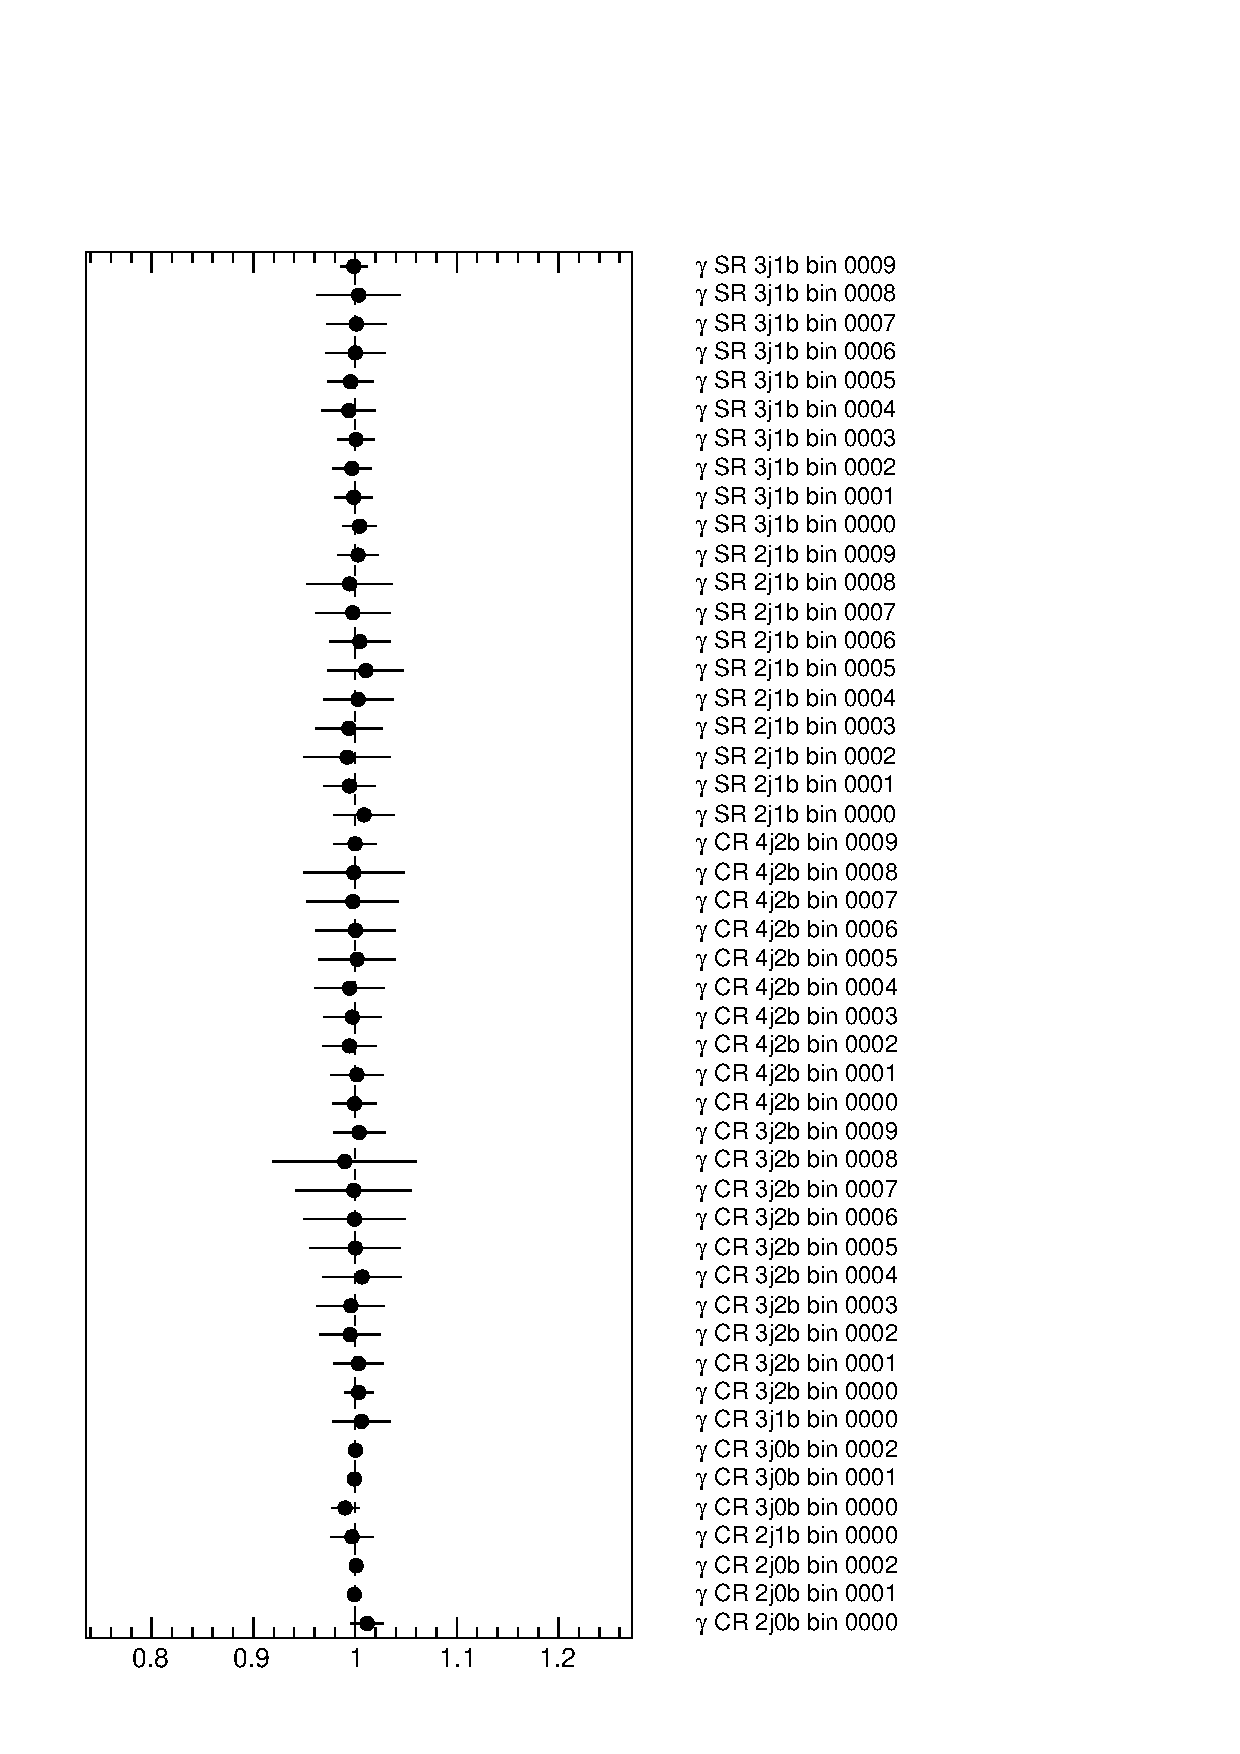
\includegraphics[width=1.1\textwidth]{ubonn-thesis/Chapters/Chapters_08/appendix/data/Gammas.pdf}
   \caption{}
   \label{fig:newgamma}
  \end{subfigure}
  \caption{(a) Pull distributions of nuisance parameters associated to systematic uncertainties using the unblinded dataset. Only nuisance parameters substantial effect are shown. (b) Pull distributions of bin gamma parameters in the unblinded fit.}
\end{figure}

\begin{figure}[!h] 
  \begin{subfigure}[b]{0.49\linewidth}
    \centering
    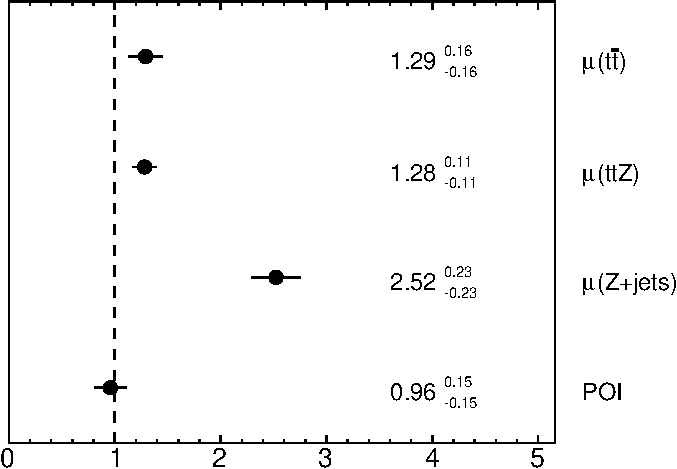
\includegraphics[width=\textwidth]{ubonn-thesis/Chapters/Chapters_08/appendix/data/NormFactors_statOnly-crop.pdf}
    \caption{}
    \label{fig:newnormfactoestat}
  \end{subfigure}%% 
  \begin{subfigure}[b]{0.49\linewidth}
    \centering
    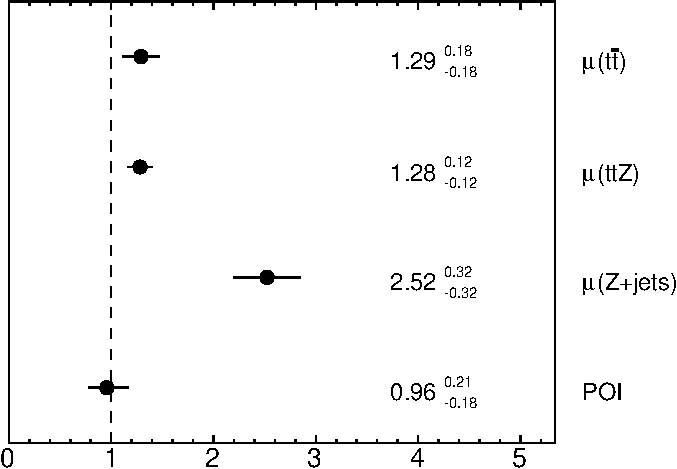
\includegraphics[width=\textwidth]{ubonn-thesis/Chapters/Chapters_08/appendix/data/NormFactors-crop.pdf}
   \caption{}
   \label{fig:newnormfactor}
  \end{subfigure}
  \caption{Norm factors of the free floating parameters used in the signal plus background fit using unblinded dataset (without neural network training). (a) Statonly fit (b) Stat + Syst fit}
\end{figure}

 
 
\begin{figure}[!h] 
  \begin{subfigure}[b]{0.33\linewidth}
    \centering
    \includegraphics[width=\textwidth]{ubonn-thesis/Chapters/Chapters_08/appendix/data/SR_2j1b.pdf} 
  \end{subfigure}%% 
  \begin{subfigure}[b]{0.33\linewidth}
    \centering
    \includegraphics[width=\textwidth]{ubonn-thesis/Chapters/Chapters_08/appendix/data/SR_3j1b.pdf} 
  \end{subfigure} 
  \begin{subfigure}[b]{0.33\linewidth}
    \centering
    \includegraphics[width=\textwidth]{ubonn-thesis/Chapters/Chapters_08/appendix/data/CR_3j2b.pdf} 
  \end{subfigure}%%
  \newline
  \begin{subfigure}[b]{0.33\linewidth}
    \centering
    \includegraphics[width=\textwidth]{ubonn-thesis/Chapters/Chapters_08/appendix/data/SR_2j1b_postFit.pdf} 
  \end{subfigure} 
  \begin{subfigure}[b]{0.33\linewidth}
    \centering
    \includegraphics[width=\textwidth]{ubonn-thesis/Chapters/Chapters_08/appendix/data/SR_3j1b_postFit.pdf} 
  \end{subfigure}%% 
  \begin{subfigure}[b]{0.33\linewidth}
    \centering
    \includegraphics[width=\textwidth]{ubonn-thesis/Chapters/Chapters_08/appendix/data/CR_3j2b_postFit.pdf} 
  \end{subfigure} 
  \newline
  \begin{subfigure}[b]{0.33\linewidth}
    \centering
    \includegraphics[width=\textwidth]{ubonn-thesis/Chapters/Chapters_08/appendix/data/CR_4j2b.pdf} 
  \end{subfigure} 
  \begin{subfigure}[b]{0.33\linewidth}
    \centering
    \includegraphics[width=\textwidth]{ubonn-thesis/Chapters/Chapters_08/appendix/data/CR_2j0b.pdf} 
  \end{subfigure}%% 
  \begin{subfigure}[b]{0.33\linewidth}
    \centering
    \includegraphics[width=\textwidth]{ubonn-thesis/Chapters/Chapters_08/appendix/data/CR_3j0b.pdf} 
  \end{subfigure} 
  \caption{ The pre-fit and post-fit distributions in the signal regions and control regions described in the table \ref{tab:newfittedregions}. The black points show the blinded dataset. The error band includes the statistical and systematic uncertainties.}
  \label{fig:newfit1}
\end{figure}

\begin{figure}[!h] 
  \begin{subfigure}[b]{0.33\linewidth}
    \centering
    \includegraphics[width=\textwidth]{ubonn-thesis/Chapters/Chapters_08/appendix/data/CR_4j2b_postFit.pdf} 
    \caption{}
  \end{subfigure}%% 
  \begin{subfigure}[b]{0.33\linewidth}
    \centering
    \includegraphics[width=\textwidth]{ubonn-thesis/Chapters/Chapters_08/appendix/data/CR_2j0b_postFit.pdf} 
    \caption{}
  \end{subfigure} 
  \begin{subfigure}[b]{0.33\linewidth}
    \centering
    \includegraphics[width=\textwidth]{ubonn-thesis/Chapters/Chapters_08/appendix/data/CR_3j0b_postFit.pdf} 
    \caption{}
  \end{subfigure}%%
  \newline
  \centering
  \begin{subfigure}[b]{0.33\linewidth}
    \includegraphics[width=\textwidth]{ubonn-thesis/Chapters/Chapters_08/appendix/data/CR_2j1b.pdf} 
    \caption{}
  \end{subfigure} 
  \centering
  \begin{subfigure}[b]{0.33\linewidth}
    \includegraphics[width=\textwidth]{ubonn-thesis/Chapters/Chapters_08/appendix/data/CR_3j1b.pdf} 
    \caption{}
  \end{subfigure}%% 
  \newline
  \hspace*{-1.5cm}
  \begin{subfigure}[b]{0.33\linewidth}
   \includegraphics[width=\textwidth]{ubonn-thesis/Chapters/Chapters_08/appendix/data/CR_2j1b_postFit.pdf} 
    \caption{}
  \end{subfigure} 
  \centering
  \begin{subfigure}[b]{0.33\linewidth}
  %\hspace*{-1.0cm}
    \includegraphics[width=\textwidth]{ubonn-thesis/Chapters/Chapters_08/appendix/data/CR_3j1b_postFit.pdf}
   \caption{}
  \end{subfigure}%% 
  \caption{Pre-fit and post-fit distributions in the signal regions and control regions described in the table \ref{tab:newfittedregions}. The black points show the blinded dataset. The error band includes the statistical and systematic uncertainties.}
  \label{fig:newfit2}
  \end{figure}

 
%In the appendix you usually include extra information that should be documented in your thesis, but not interrupt the flow.

%%% Local Variables: 
%%% mode: latex
%%% TeX-master: "../mythesis"
%%% End: 
